%%%%%%%%%%%%%%%%%%%%%%%%%%%%%%%%%%%%%%%%%%%%%%%%%%%%%%%%%%%%%%%
%
% Welcome to Overleaf --- just edit your LaTeX on the left,
% and we'll compile it for you on the right. If you open the
% 'Share' menu, you can invite other users to edit at the same
% time. See www.overleaf.com/learn for more info. Enjoy!
%
%%%%%%%%%%%%%%%%%%%%%%%%%%%%%%%%%%%%%%%%%%%%%%%%%%%%%%%%%%%%%%%
\documentclass[12pt,a4paper,oneside]{book}


\usepackage[T1]{fontenc}
\usepackage[utf8]{inputenc}
\usepackage{arabtex}
\usepackage{utf8}
\setcode{utf8}
% \usepackage{babel}
\usepackage[french]{babel}
\usepackage{svg}
\usepackage{amsmath}
\usepackage{amsthm}
\usepackage{amssymb}
\usepackage{tikz}
\usepackage{tcolorbox}
\usepackage{tabularx}
\usetikzlibrary{calc}
\usepackage[french,ruled,vlined]{algorithm2e}
\usepackage{rotating}
\usepackage{bbding}
\usepackage{cite}
\usepackage{lscape,graphicx}
\usepackage{rotating}
\usepackage{setspace}
\usepackage{sectsty}
\usepackage{dsfont}
\usepackage{ifpdf}
\usepackage{subfigure}
\usepackage{epsfig}
\usepackage{float}
\usepackage{titlesec}
\usepackage{multibib}
\usepackage{fancyhdr}
\usepackage{lipsum}
\usepackage{soul}
\usepackage[paperwidth=210mm,paperheight=297mm,tmargin=15mm,lmargin=20mm]{geometry}
%
\renewcommand{\topfraction}{0.9}
\renewcommand{\textfraction}{0.1}
\renewcommand{\floatpagefraction}{0.8}
%

\usepackage{hyperref}


\urlstyle{same}

\setlength{\headheight}{30pt}
\pagestyle{fancy}% \renewcommand{\chaptermark}[1]{\markboth{#1}{}}
\renewcommand{\chaptermark}[1]{\markboth{\MakeUppercase{#1}}{}}
\renewcommand{\sectionmark}[1]{\markright{\MakeUppercase{\thesection.\ #1}}}


%
% \renewcommand{\sectionmark}[1]{\markright{#1}}
%\renewcommand \thesection{\Roman{section}.}
%\renewcommand \thesubsection{\alph{subsection}.}
%
%\newcommand{\helv}{%
%\fontfamily\fontsize{9}{11}\selectfont}

%

% Clear Header Style on the Last Empty Odd pages
\makeatletter
\def\cleardoublepage{\clearpage\if@twoside \ifodd\c@page\else%
            \hbox{}%
            \thispagestyle{empty}%              % Empty header styles
            \newpage%
            \if@twocolumn\hbox{}\newpage\fi\fi\fi}
\makeatother


\fancyhead[RE]{\textit{\nouppercase{\leftmark}}}
\fancyhead[LO]{\textit{\nouppercase{\rightmark}}}
\fancyhead[LE,RO]{\thepage}

\renewcommand{\headrulewidth}{0pt}
\renewcommand{\footrulewidth}{0pt}
%
\setcounter{secnumdepth}{4}
\setcounter{tocdepth}{4}
%

%
\def\ds{\displaystyle}
\def\dir{./figures}

%


%\setlength\topmargin{0in}
%\setlength\topmargin{0in}
%

%
% Remove page numbering from first page Bibliography
%
%%%%%%%%%%%%%%%%%%%%%%%%% Page de titre %%%%%%%%%%%%%%%%%%%%%%%
\def\baselinestretch{1.5}


\usepackage{listings}
\usepackage{caption}
\usepackage{longtable}

\usepackage{geometry}
\usepackage{booktabs}

\geometry{
    letterpaper,
    left=1.5cm,
    right=1.5cm,
    top=1.5cm,
    bottom=1.5cm
}

\usepackage{afterpage}

\newcommand\blankpage{%
    \null
    \thispagestyle{empty}%
    \addtocounter{page}{-1}%
    \newpage}


\usepackage[acronym]{glossaries}

\usepackage{lmodern}


\newenvironment{dedication}
{%\clearpage           % we want a new page          %% I commented this
    \thispagestyle{empty}% no header and footer
    \vspace*{\stretch{1}}% some space at the top
    \itshape             % the text is in italics
    \raggedleft          % flush to the right margin
}
{\par % end the paragraph
    \vspace{\stretch{3}} % space at bottom is three times that at the top
    \clearpage           % finish off the page
}






%\makenoidxglossaries 

%\newglossaryentry{latex}
%{
       % name=latex,
        %description={Is a mark up language specially suited for scientific documents}
%}



\selectlanguage{francais}



\hypersetup{
    colorlinks=true,
    linkcolor=black,
    filecolor=magenta,      
    urlcolor=cyan,
    pdfauthor={Anass REBBAG},  %put your name here
    pdftitle={Rapport de stage de fin d'études},  %PDF title
    pdfpagemode=FullScreen,
    }



\begin{document}



\definecolor{codegreen}{rgb}{0,0.6,0}
\definecolor{codegray}{rgb}{0.5,0.5,0.5}
\definecolor{codepurple}{rgb}{0.58,0,0.82}
\definecolor{backcolour}{rgb}{0.95,0.95,0.92}

\lstdefinestyle{mystyle}{
    backgroundcolor=\color{backcolour},
    keywordstyle=\color{magenta},
    numberstyle=\tiny\color{codegreen},
    stringstyle=\color{codepurple},
    basicstyle=\ttfamily\footnotesize,
    breakatwhitespace=false,
    breaklines=true,
    captionpos=b,
    keepspaces=true,
    numbers=left,
    numbersep=5pt,
    showspaces=false,
    showstringspaces=false,
    showtabs=false,
    tabsize=2
}




%
\thispagestyle{empty}

\includegraphics[scale=0.08]{Logos/Logo_INPT.png}
\hspace{11cm}

\includegraphics[scale=0.1]{Logos/b3g-vector-logo.png}

\vspace{0.9cm}
\begin{center}
    {\large \textsc{\textbf{Mémoire de projet de fin d'études}}}\\[0.1cm]
    {\large \textsc{Pour L'obtention du Diplôme d'Ingénieur d'État en Télécommunications et Technologies de l'Information }}\\[0.1cm]
    {\large \textsc{\textit{Filière : Systèmes et services numériques}}} \\[0.05cm]
    \vspace{-0.04cm}
    % Title
    \rule{\linewidth}{0.3mm} \\[0.4cm]   % à ajuster l'éspace en cas de besoin: [1cm]
    { \large \textbf{ Développement d'une plateforme low-code Fawri CMS pour des solutions bancaires numériques }} \\[0.01cm]
    \rule{\linewidth}{0.3mm} \\[0.4cm]
    \vspace{0.4cm}

    %
\includegraphics[scale=0.075]{Logos/Company_Logo_Expl.png}  %change the scale to suit your logo

    \vspace{1cm}

    % Author and supervisor
    \noindent
    \begin{minipage}{0.9\textwidth}
        \vspace{-7mm}
        \begin{flushleft} \large
            \emph{Réalisé par :}\\
            M. Anass \textsc{REBBAG} %\& Mme / M. Xxxx \textsc{XXXX}  %Au cas de binôme, remove the % \\
        \end{flushleft}
    \end{minipage}
    \begin{minipage}{0.4\textwidth}

    \end{minipage}\\[0.6cm]

    {\large \textit{Soutenu le 12 Juillet 2024, devant le jury composé de : }}\\[0.5cm]


    \begin{tabular}{p{1cm}lll}
         & \large Pr. Safae \textsc{DAHMANI}   & \large INPT       & \large - Examinatrice \\[0.1cm]
         & \large Pr. Najib \textsc{NAJA}      & \large INPT       & \large - Examinateur  \\[0.1cm]
         & \large Pr. Yann \textsc{BEN MAISSA} & \large INPT       & \large - Encadrant    \\[0.1cm]
         & \large M. Rida \textsc{ABOUZID}     & \large Entreprise & \large - Encadrant    \\[0.1cm]
    \end{tabular}

    \vspace{0.5cm}
    
\includegraphics[scale=0.6]{Logos/ZLAFA.png}


    %\textsc{Agence Nationale de Réglementation des Télécommunications}\\
    \textsc{Institut National des Postes et Télécommunications}
    % Bottom of the page

    %\vspace{0.3cm}
    {\large Promotion : 2023/2024}

\end{center}


 %FRENCH ONE


\thispagestyle{empty}

\includegraphics[scale=0.08]{Logos/Logo_INPT.png}
\hspace{11cm}

\includegraphics[scale=0.1]{Logos/b3g-vector-logo.png}

\vspace{0.9cm}
\begin{center}
    {\large \textsc{\textbf{Mémoire de projet de fin d'études}}}\\[0.1cm]
    {\large \textsc{Pour L'obtention du Diplôme d'Ingénieur d'État en Télécommunications et Technologies de l'Information }}\\[0.1cm]
    {\large \textsc{\textit{Filière : Systèmes et services numériques}}} \\[0.05cm]
    \vspace{-0.04cm}
    % Title
    \rule{\linewidth}{0.3mm} \\[0.4cm]   % à ajuster l'éspace en cas de besoin: [1cm]
    { \large \textbf{ Développement d'une plateforme low-code Fawri CMS pour des solutions bancaires numériques }} \\[0.01cm]
    \rule{\linewidth}{0.3mm} \\[0.4cm]
    \vspace{0.4cm}

    %
\includegraphics[scale=0.075]{Logos/Company_Logo_Expl.png}  %change the scale to suit your logo

    \vspace{1cm}

    % Author and supervisor
    \noindent
    \begin{minipage}{0.9\textwidth}
        \vspace{-7mm}
        \begin{flushleft} \large
            \emph{Réalisé par :}\\
            M. Anass \textsc{REBBAG} %\& Mme / M. Xxxx \textsc{XXXX}  %Au cas de binôme, remove the % \\
        \end{flushleft}
    \end{minipage}
    \begin{minipage}{0.4\textwidth}

    \end{minipage}\\[0.6cm]

    {\large \textit{Soutenu le 12 Juillet 2024, devant le jury composé de : }}\\[0.5cm]


    \begin{tabular}{p{1cm}lll}
         & \large Pr. Safae \textsc{DAHMANI}   & \large INPT       & \large - Examinatrice \\[0.1cm]
         & \large Pr. Najib \textsc{NAJA}      & \large INPT       & \large - Examinateur  \\[0.1cm]
         & \large Pr. Yann \textsc{BEN MAISSA} & \large INPT       & \large - Encadrant    \\[0.1cm]
         & \large M. Rida \textsc{ABOUZID}     & \large Entreprise & \large - Encadrant    \\[0.1cm]
    \end{tabular}

    \vspace{0.5cm}
    
\includegraphics[scale=0.6]{Logos/ZLAFA.png}


    %\textsc{Agence Nationale de Réglementation des Télécommunications}\\
    \textsc{Institut National des Postes et Télécommunications}
    % Bottom of the page

    %\vspace{0.3cm}
    {\large Promotion : 2023/2024}

\end{center}


 % ENGLISH

\afterpage{\blankpage}  %page vide obligatoire

\frontmatter


\chapter*{Dédicaces}
\addcontentsline{toc}{chapter}{Dédicaces}

  \begin{dedication}
  
    À mes chers parents et à chaque membre précieux de ma famille,

Avec tout mon amour, je vous dédie ce travail. Votre soutien indéfectible, votre amour inconditionnel et vos prières incessantes ont illuminé mon parcours et ont été les fondements de ma réussite.

    \vspace{1\baselineskip}
À mes meilleurs amis,

Votre présence constante, votre amitié fidèle et votre encouragement infaillible ont été une source de force et de motivation tout au long de ce voyage.

À toutes les personnes qui ont contribué de près ou de loin à ce travail,

Votre soutien et votre collaboration ont été inestimables et je vous en suis profondément reconnaissant.

Que cette dédicace soit le témoignage de mon respect et de ma reconnaissance envers vous tous qui avez joué un rôle essentiel dans mon parcours académique, et de vie.
    
    \par   %% or a blank line


    \vspace{\baselineskip}
    \usefont{T1}{LobsterTwo-LF}{bx}{it} Anass REBBAG.
  \end{dedication}





\chapter*{Remerciements}
\addcontentsline{toc}{chapter}{Remerciements}

\hspace{\parindent} À l'issue de ce stage, je tiens à exprimer ma profonde gratitude envers Madame \textbf{Dania ELGHISSASSI, Monsieur Doraid Seddiki} et \textbf{Monsieur Faycal Bellamine}, pour leur généreuse contribution à la réalisation de mon projet de fin d'études au sein de B3G. Leur soutien et leurs conseils ont été d'une aide inestimable.

Je souhaite également exprimer ma sincère gratitude envers Monsieur \textbf{Yann BEN MAISSA}, mon encadrant interne et professeur, pour son soutien indéfectible tout au long de cette période. Je lui suis infiniment reconnaissant pour son suivi attentif, son engagement constant, ses conseils éclairés, et son encouragement permanent, qui ont été les fondements de cet encadrement de qualité. Ses cours ont également grandement contribué à ma réussite, en me fournissant une solide base de connaissances et en m'aidant à développer des compétences essentielles pour ce stage. Ses enseignements ont joué un rôle crucial dans la compréhension et l'application des concepts nécessaires pour mener à bien mes projets.

Je suis reconnaissant aux membres du jury, Mme \textbf{DAHMANI Safae} et Pr. \textbf{NAJA Najib} pour leur participation à l'évaluation de ce rapport de stage et la supervision de ma présentation. Leur temps et leurs commentaires réfléchis sont grandement appréciés.

Je tiens également à exprimer ma sincère gratitude envers Monsieur \textbf{ABOUZID Reda} et Monsieur \textbf{Abdelhadi BABENGHANMI}, mes encadrants à B3G, pour leurs précieux conseils, leurs recommandations avisées et leur soutien inébranlable tout au long de mon projet de fin d’études. Leur expertise et leur accueil chaleureux ont été d'une valeur inestimable pour mon développement professionnel.


Je remercie également toute l'équipe de B3G pour leur accueil chaleureux et leur précieuse assistance tout au long de mon stage. Leur disponibilité et leur volonté de partager leur expertise ont grandement enrichi mon parcours professionnel.

Enfin, je souhaite exprimer ma gratitude envers mes parents, mes amis et tous ceux qui m'ont conseillé et relu attentivement le présent rapport de projet de fin d’études pour m’aider à en améliorer la qualité et la consistance. A tous je vous dis merci.




\chapter*{Résumé}
\addcontentsline{toc}{chapter}{Résumé}

\hspace{\parindent} Ces dernières années, le secteur bancaire a connu une poussée significative vers la transformation numérique, nécessitant des solutions innovantes pour répondre aux besoins technologiques en constante évolution.

Ce rapport présente le développement de Fawri CMS, une solution numérique de pointe adaptée à l'industrie bancaire, élaborée au sein de l'entreprise B3G dans le cadre de mon stage de fin d'études. Fawri-CMS simplifie le développement d'applications grâce à une approche "Low Code", permettant aux développeurs de créer des applications robustes avec un minimum de codage manuel tout en intégrant de manière transparente des processus métier complexes.Le système propose des fonctionnalités avancées de gestion de contenu (CMS) telles que la création, la gestion et la publication de contenu, conçues pour répondre à des normes de sécurité et de conformité strictes.

Le projet a suivi une méthodologie de gestion de projet agile, en particulier le cadre SCRUM, facilitant le développement itératif et les boucles de rétroaction régulières. Le parcours a débuté par une phase d’analyse et de conception approfondie utilisant des diagrammes UML pour modéliser l’architecture du système, suivie de la conception technique et de la configuration de l’environnement de développement, incluant SQL Server et .NET Core.
La phase de développement a impliqué l'application des principes de la conception pilotée par le domaine (DDD) pour garantir la résilience et la maintenabilité du système. Un aspect remarquable a été la mise en œuvre de la fonctionnalité de création de formulaires, permettant de glisser-déposer des composants, en utilisant JavaScript. Ce composant a ensuite été publié sur npm et intégré de manière transparente à notre solution .NET, en harmonie avec les autres fonctionnalités du CMS.

\noindent\rule[2pt]{\textwidth}{0.5pt}

{\textbf{Mots clés :}}
Secteur bancaire, transformation digitale, approche Low Code, business processes, CMS, SQL Server, .NET Core, DDD.
\\
\noindent\rule[2pt]{\textwidth}{0.5pt}

% \cleardoublepage
%

\chapter*{Summary}
\addcontentsline{toc}{chapter}{Summary}

\hspace{\parindent}  In recent years, the banking sector has seen a significant push towards digital transformation, requiring innovative solutions to meet evolving technological demands.

This report presents the development of Fawri-CMS, a cutting-edge digital solution tailored for the banking industry, developed within the company B3G as part of my final graduation internship. A CMS, or Content Management System, allows users to create, manage, and modify content on a website without needing extensive technical knowledge. Fawri-CMS simplifies application development through a Low-Code approach, which utilizes visual development tools and pre-configured templates, enabling developers to create robust applications with minimal hand-coding and seamlessly integrating complex business processes. The system offers advanced CMS features such as content creation, management, and publication, designed to meet stringent security and compliance requirements.

The project followed an agile project management methodology, specifically the SCRUM
framework, enabling iterative development and regular feedback. We began with a detailed analysis and design phase, utilizing UML diagrams to model the system’s architecture. This was followed by technical design and the setup of the development environment, including SQL Server and .NET Core.
The development process involved the implementation of Domain-Driven Design (DDD) principles to ensure the robustness and maintainability of the system. A significant part of the form-building functionality, which allows for drag-and-drop components, was developed using JavaScript. This component was then published to npm and subsequently imported into our .NET solution, integrating seamlessly with the broader CMS features.

\noindent\rule[2pt]{\textwidth}{0.5pt}

\textbf{Keywords :}
Banking sector, digital transformation, Low-Code approach, business
processes, CMS, SQL Server, .NET Core, DDD.
\\
\noindent\rule[2pt]{\textwidth}{0.5pt}

% \cleardoublepage
%


\chapter*{\RL{ملخص}}
\addcontentsline{toc}{chapter}{Résumé en Arabe}

\begin{RLtext}
في السنوات الأخيرة، شهد قطاع البنوك دفعة كبيرة نحو التحول الرقمي، مما يتطلب حلولًا مبتكرة لتلبية الاحتياجات التكنولوجية المتطورة. يبرز هذا التقرير تطوير \LR{Fawri-CMS} الحل الرقمي المتقدم المصمم خصيصًا لصناعة البنوك والذي تم تطويره داخل شركة \LR{B3G} خلال فترة تدريبي النهائية.

يبسط \LR{Fawri-CMS} تطوير التطبيقات من خلال منهجية \LR{"Low-Code"} مما يمكن المطورين من بناء تطبيقات قوية مع الحد الأدنى من البرمجة اليدوية مع دمج سلس للعمليات التجارية المعقدة. يتميز النظام بميزات متقدمة لنظام إدارة المحتوى \LR{(CMS)} بما في ذلك إنشاء المحتوى وإدارته ونشره، مصممة بدقة لتلبية معايير الأمان والامتثال الصارمة.

اعتمد المشروع منهجية إدارة مشاريع البرمجيات الرشيقة والمضبوطة \LR{SCRUM} مما يسهل التطوير التكراري وحلقات الردود الدورية. بدأت الرحلة بمرحلة تحليل وتصميم دقيقة باستخدام مخططات \LR{UML} لنمذجة هندسة النظام، تلاها التصميم الفني وإعداد بيئة التطوير، بما في ذلك \LR{SQL Server} و \LR{.NET Core}.

شملت مرحلة التطوير تنفيذ مبادئ التصميم القائم على المجال \LR{DDD} لضمان قوة النظام وقابليته للصيانة. كان جزءاً هاماً من وظائف بناء النماذج، التي تتيح إسقاط المكونات، مطورًا باستخدام \LR{JavaScript}. ثم يتم تقييد هذا المكون على \LR{npm} ودمجه ببساطة مع الميزات الأخرى لنظام إدارة المحتوى.


\end{RLtext}

\noindent\rule[2pt]{\textwidth}{0.5pt}

\begin{RLtext} 

{\textbf{الكلمات المفتاحية}}
 قطاع البنوك، التحول الرقمي، نهج "الكود المنخفض"، عمليات الأعمال، نظام إدارة المحتوى.

\\

\end{RLtext}

\noindent\rule[2pt]{\textwidth}{0.5pt}

% \cleardoublepage
%






\listoffigures
\addcontentsline{toc}{chapter}{Liste des Figures}
%figures are added automatically here

\listoftables
\addcontentsline{toc}{chapter}{Liste des Tables}
%tables are added automatically here

% \lstlistoflistings
% \addcontentsline{toc}{chapter}{List of Listings} 
% %Code snippets are added automatically here


\chapter{Glossaire}
\label{chap:Glossary}


\hspace{\parindent}\textbf{CMS:} CMS est l’acronyme de Content Management System, c’est-à-dire système de gestion de contenu. Il s’agit d’un logiciel en ligne grâce auquel il est possible de créer, de gérer et de modifier facilement un site web, sans avoir besoin de connaissances techniques en langage informatique.\\

\textbf{Low Code:} c'est une approche de développement logiciel qui permet de créer des applications rapidement avec un minimum de programmation manuelle. Cette méthode utilise des outils de développement visuels pour permettre aux utilisateurs de créer des applications en drag-and-drop, en cliquant sur des éléments de l’interface graphique et en utilisant des blocs de code préconstruits.\\

\textbf{DDD:} (Domain-Driven Design) est une approche de conception logicielle centrée sur la compréhension et la modélisation approfondies du domaine d'application. Elle met en avant l'utilisation d'un modèle de domaine précis et riche, un langage ubiquitaire partagé par les développeurs et les experts du domaine, et des contextes délimités pour organiser le modèle en sous-domaines cohérents.\\


\textbf{L'approche TDD :} (Test-Driven Development) est une approche de développement logiciel qui consiste à écrire des tests automatisés avant d'écrire le code fonctionnel. Le processus commence par la rédaction d'un test unitaire qui spécifie et valide ce que le code doit accomplir. Ensuite, le développeur écrit le code minimal nécessaire pour faire passer ce test. Une fois le test réussi, le code est refactorisé pour améliorer sa structure tout en s'assurant que les tests continuent à passer.\\


\pagebreak

\chapter{Acronyms}

%Example of Acronyms using table 

\begin{tabular}{l l}

% page 1

\textbf{CMS} & Content Management System \\
\textbf{CSRF} & Cross-site request forgery \\
\textbf{DDD} & Domain Driven Design \\



\textbf{DTO} & Data Transfer Object \\

\textbf{EF} & Entity Framework \\

\textbf{IDE} & Integrated Development Environment \\

\textbf{KYC} & Know Your Customer \\

\textbf{RDBMS} & Relational Database Management System \\

\textbf{SAAS} & Software As a Service \\

\textbf{SSMS} & SQL Server Management Studio \\

\textbf{TBD} & Trunk-based development \\
\textbf{TDD} & Test Driven Development \\


\textbf{UML} & Unified Modeling Language \\

\textbf{UI} & User Interface \\

\textbf{UX} & User Experience \\

\textbf{WS} & Web Service \\

\textbf{WYSIWYG} & What You See Is What You Get \\

\textbf{XSS} & Cross-site scripting \\


% end of page 1

\end{tabular}

\pagebreak




\tableofcontents
\addcontentsline{toc}{chapter}{Table des matières}
%contents are added automatically here




\mainmatter

%debut of chapters


\chapter*{Introduction générale}

\addcontentsline{toc}{chapter}{Introduction générale }

\label{chap: Conclusion générale} 


\hspace{\parindent}La transformation digitale est devenue un impératif stratégique pour le secteur bancaire, sous l'impulsion de régulations et de normes établies, notamment par le Groupement Professionnel des Banques du Maroc (GPBM). Dans ce cadre, B3G, une entreprise spécialisée dans le développement de solutions digitales pour les banques, a conçu la suite Fawri-Flow pour moderniser et optimiser les opérations bancaires.

Afin de répondre aux besoins croissants de cette transformation digitale et de faciliter la gestion de contenus et processus métiers complexes, il est apparu nécessaire de développer un CMS Low-Code. Cette démarche a conduit à la réalisation de notre projet de fin d’études, portant sur le développement de Fawri-CMS, une solution innovante et flexible.

Fawri-CMS vise à simplifier le processus de développement d'applications grâce à une approche "Low-Code" et à intégrer les processus métier de manière transparente. Cela permet de réduire significativement le temps et les ressources nécessaires au développement. La solution permet également à un plus grand nombre d'utilisateurs de créer des applications adaptées à leurs besoins spécifiques, ce qui lui a valu une reconnaissance notable lors du \textbf{"Saudi No Code Innovation Summit"}.

Ce rapport présente les différentes étapes de la réalisation de cette solution, en mettant en lumière les choix et décisions prises tout au long du projet, ainsi que les résultats obtenus. Il est structuré en quatre chapitres principaux :
\begin{itemize}
\item \textbf{Présentation Générale}

Ce chapitre contextualise le projet, présentant les objectifs du stage, l'entreprise B3G, et l'application à développer. Il aborde également les enjeux de la transformation digitale, les concepts de Low-Code et de CMS, ainsi que les choix technologiques et méthodologiques retenus pour mener à bien le projet.

\item \textbf{Analyse et Conception}

Ce chapitre se concentre sur l'analyse détaillée des besoins fonctionnels de l'application. Il inclut la modélisation conceptuelle des différents domaines fonctionnels, identifiant les classes, les relations, et les processus métier impliqués.

\item \textbf{Outils, Méthodologies et Architecture}

Ici, l'accent est mis sur les outils, les méthodologies et l'architecture utilisés lors du développement de l'application. Le chapitre décrit les technologies employées, telles que le framework .NET et ABP, ainsi que les principes de conception comme TDD, SOLID, et DDD. L'architecture logicielle est expliquée en soulignant les choix architecturaux et les bonnes pratiques adoptées.

\item \textbf{Implémentation et Réalisation}

Ce dernier chapitre se focalise sur l'implémentation de l'application. Il détaille les étapes de développement, les fonctionnalités implémentées, les tests réalisés, et les résultats obtenus. Une rétrospective sur le déroulement du projet et les résultats est également incluse.
\end{itemize}
Ce rapport a pour but de fournir une vue d'ensemble complète de la création et du développement de Fawri-CMS, tout en illustrant les défis rencontrés et les solutions apportées pour les surmonter.


\chapter{Présentation générale}
\label{chap:Présentation générale}

% "*" makes the section unnumbered

\section*{Introduction}

\hspace{\parindent}Ce chapitre introduit notre rapport de projet de fin d'études. Nous commençons par présenter l'organisme d'accueil, B3G, en mettant en lumière ses solutions et sa clientèle. Ensuite, nous délimitons le cadre du projet et exposons la problématique à laquelle notre travail vise à répondre. Nous décrivons ensuite la solution proposée et les étapes de sa mise en œuvre. Enfin, nous abordons la conduite du projet, incluant le calendrier prévu et les étapes clés à venir. Cette introduction permet de comprendre le contexte global et de poser les bases pour la suite de notre rapport.
\newpage

\section{Présentation de l'entreprise}

\hspace{\parindent}Cette section présente l'organisme d'accueil du stage - B3G Tech, Omni Channel Digital Banking and Wallet.

\subsection{B3G Tech}

\hspace{\parindent}Fondée en 2004, B3G (cf. Figure 1) est une société de services spécialisée dans l'édition, l'intégration et l'optimisation de solutions digitales pour le secteur bancaire. Elle propose une solution omnicanale de banque digitale et de Mobile Money à travers sa suite d'applications intégrée, Fawri, qui permet une gestion unifiée de l'expérience client via divers canaux : Mobile, Web, SMS, Voix, Email et Kiosque.




%Use \paragraph{To start a paragraph}

\begin{figure}[H]
    \centering
    
\includegraphics[width=10cm]{Logos/B3G.png}
    \caption{B3G Digital Banking \& wallet}
    \label{fig:my_label} %Optional (If you want to reference the figure in later chapters)
\end{figure}

%[width=7cm] you control the size of the image. other options include: 
%[height=7cm] or [scale=0.5] (means half the size of the original image)


% Documentation: \href{https://www.overleaf.com/learn/latex/Inserting_Images}{Images}



% \begin{tabular}{ll}
%   First & Second \\
%   Third & Fourth
% \end{tabular}
% \\

% More complex table with borders:


% \begin{tabular}{|l|c|r|} \hline
%   Left aligned column & Centered column & Right aligned column \\ \hline
%   Text & Text & Text \\ \hline
% \end{tabular}
% \\

% Example of a short table

%{5cm} is the cell length, you can change it to suit your own table

\begin{table}[H]
    \centering
    \begin{tabular}{|m{5cm}|m{10cm}|}
        \hline
        Site web               & \href{https://b3gtech.com/}{B3G Tech } \\
        \hline
        Siège social           & Rabat                                  \\
        \hline
        Année de création      & 2004                                   \\
        \hline
        Type d'entreprise      & société privée / SARL                  \\
        \hline
        Taille de l'entreprise & 51-200 employés                        \\
        \hline
        Implantations          & Rabat, Casablanca, Paris               \\
        \hline
    \end{tabular}
    \caption{Fiche de l'entreprise}
\end{table}


% Example of a long table (that spans 2 pages or more), Latex will automatically split the table when it reaches the end of the page:

% \begin{longtable}[c]{| m{4.4cm} | m{11cm} |}
% \caption{Long table}\\
%  \hline

%  Cell & Description  \\ 
%  \hline
%  \endfirsthead

%  \hline

%  Cell & Description  \\ 
%  \hline
%  \endhead

%         \hline
%           Element11 & Element21 \\
%         \hline
%           Element12 & Element22 \\
%         \hline
%           Element13 & Element23 \\
%         \hline
%           Element14 & Element24 \\
%         \hline
%           Element15 & Element25 \\
%         \hline
%           Element16 & Element26 \\
%         \hline
%           Element17 & Element27 \\
%         \hline
%           Element18 & Element28 \\
%         \hline
%           Element19 & Element29 \\
%         \hline
%           Element110 & Element210 \\
%         \hline
%           Element111 & Element211 \\
%         \hline
%           Element112 & Element212 \\
%         \hline
%           Element113 & Element213 \\
%         \hline
%           Element114 & Element214 \\
%         \hline

%  \end{longtable}


% Documentation: \href{https://www.overleaf.com/learn/latex/Tables}{Tables}

\subsection{Produits \& Solutions}

\hspace{\parindent}B3G propose une gamme complète de solutions packagées regroupées sous la suite applicative FawriSuite. Cette suite Omnicanal offre une solution de Banque Digitale et Mobile Money entièrement intégrée, permettant de gérer de manière unifiée l'ensemble de l'expérience client à travers différents canaux tels que le mobile, le web, les SMS, la voix, l'e-mail et les kiosques. Parmi les solutions phares de la gamme FawriSuite, on retrouve FawriBank, FawriWallet et FawriAlert, qui couvrent respectivement les aspects de la banque digitale, du portefeuille électronique et des notifications transactionnelles.

FawriSuite, créée par B3G, est une plateforme informatique éprouvée destinée aux institutions financières, aux opérateurs de télécommunications, aux opérateurs de services publics et aux agences gouvernementales. Basée sur une Architecture Orientée Service (SOA), FawriSuite est une solution centrée sur le client, offrant flexibilité et visibilité à son expérience. Elle répond de manière personnalisée aux besoins spécifiques de chaque client à tous les points de contact.

La gamme FawriSuite propose des solutions packagées couvrant tous les aspects de la banque digitale :
\begin{itemize}
    \item \textbf{Fawri Bank}: Une solution Omnicanal intégrée de banque digitale offrant des services tels que l'E-Banking, le Mobile Banking, le SMS Banking, le Phone Banking, le Branch Banking et le Kiosk Banking, adaptée aux particuliers, professionnels et entreprises.
    \item \textbf{Fawri Wallet}: Une solution Core Banking \& Digitale front2back optimisée pour les comptes mobiles. Elle permet de gérer tout l'écosystème Mobile Money, y compris la gestion des agents et des commerçants, les fonctionnalités e-Commerce et le paiement mobile, favorisant ainsi l'inclusion financière et les stratégies CashLess.
    \item \textbf{Fawri Flow}:Une plate-forme Low-Code accélérant la digitalisation des processus, offrant ainsi une meilleure efficacité opérationnelle et une agilité accrue dans la transformation digitale des entreprises.


\end{itemize}



\begin{figure}[H]
    \centering
    
\includegraphics[width=3.5cm]{Logos/fawri.png}
    \caption{Fawri by B3G}
    \label{fig:my_label} %Optional (If you want to reference the figure in later chapters)
\end{figure}

\subsection{Clients de B3G}
\hspace{\parindent}B3G compte parmi ses clients de premier plan plusieurs institutions bancaires prestigieuses, notamment CIH Bank, Crédit Agricole du Maroc, BMCE Bank Of Africa, Umnia Bank,

LanaCash, et bien d'autres. En plus de ces institutions, B3G entretient des collaborations avec divers clients variés, tels que Veolia, Amendis et Dubai Plus.

\begin{figure}[H]
    \centering
    
\includegraphics[width=12cm]{Figures/clients.png}
    \caption{Clients de B3G}
    \label{fig:my_label} %Optional (If you want to reference the figure in later chapters)
\end{figure}

\subsection{B3G R\&D}

\hspace{\parindent}La division de recherche et développement de B3G se concentre avant tout sur la création de technologies qui permettront à B3G de rester à la pointe du secteur bancaire. Les chercheurs de B3G R\&D s'appuient sur des méthodologies et des approches innovantes, s'attaquant souvent à des défis ou des projets difficiles à réaliser au sein d'une organisation de développement de produits, ou impliquant un risque élevé ou une incertitude. La recherche de B3G R\&D se concentre sur des applications concrètes, et les chercheurs travaillent à la création de technologies qui auront un impact important sur l'évolution future de la société et de la technologie.

\section{Contexte général du projet}
\subsection{La transformation digitale des banques}

\hspace{\parindent}Le secteur bancaire a subi une transformation numérique remarquable ces dernières années, impulsée par les avancées technologiques, les évolutions des préférences des clients et les pressions concurrentielles. Cette métamorphose a radicalement modifié les modes opératoires des banques, leurs prestations de services et leurs interactions avec la clientèle.

\textbf{A. Évolution de la Banque Numérique :}

Traditionnellement, les opérations bancaires se déroulaient principalement dans des agences physiques, avec des processus manuels et des échanges en personne. Cependant, l'avènement des technologies numériques a métamorphosé les banques, les poussant à migrer des agences traditionnelles en dur vers des plateformes virtuelles.


\textbf{B. Facteurs de Transformation Numérique :}

Plusieurs éléments ont accéléré cette transformation dans le secteur bancaire :
\begin{itemize}
    \item \textbf{Attentes des Clients}: Les clients d'aujourd'hui exigent des expériences bancaires fluides, personnalisées et accessibles à tout moment et en tout lieu.
    \item \textbf{Concurrence}: L'émergence de start-ups fintech et de banques en ligne a intensifié la concurrence, incitant les banques traditionnelles à innover et à numériser leurs services.
    \item \textbf{Environnement Réglementaire}: Les changements réglementaires, notamment les initiatives de banque ouverte et les règles sur la protection des données, ont incité les banques à adopter des solutions numériques pour se conformer aux normes en évolution.
\end{itemize}


\textbf{C. Impact sur les Services Bancaires :}

La transformation numérique a entraîné des changements majeurs dans les services bancaires :
\begin{itemize}
    \item \textbf{Banque en ligne}: Les clients bénéficient désormais d'un large éventail de services bancaires en ligne, comme la gestion de compte, les paiements, les transferts de fonds et les demandes de prêt, via des plateformes sécurisées et des applications mobiles.
    \item \textbf{Expériences Personnalisées}: Les technologies d'analyse avancées et d'intelligence artificielle permettent aux banques de proposer des recommandations de produits sur mesure, des campagnes marketing ciblées et un service client proactif, améliorant ainsi l'expérience globale des clients.
    \item \textbf{Automatisation}: L'automatisation des processus manuels a conduit à une efficacité opérationnelle accrue, à des coûts réduits et à des délais de traitement plus rapides pour diverses transactions et services bancaires.
\end{itemize}



\subsection{Technologie Low-Code}

\hspace{\parindent}Les plates-formes de développement low-code occupent désormais une place centrale dans l'évolution de l'industrie logicielle, transformant fondamentalement la manière dont les applications sont conçues et déployées. Ces outils visuels facilitent la création, la modification et le déploiement d'applications même pour ceux qui ne possèdent pas de compétences en programmation, nécessitant très peu, voire aucun, codage.

En substance, ces plates-formes représentent un environnement de développement où les applications sont principalement configurées à l'aide d'interfaces graphiques plutôt que de lignes de code. Elles permettent aux utilisateurs de composer des applications à partir de composants préconstruits, en les reliant et en configurant les flux de travail de manière graphique.

\textbf{A. Les avantages du développement low-code :}

Les plateformes low-code sont précieuses, car elles rendent le développement accessible aux personnes qui n'ont pas forcément de compétences en codage, tout en permettant aux organisations de livrer des applications rapidement. Voici leurs principaux avantages :

\begin{itemize}
    \item \textbf{Rapidité}: Les outils low-code réduisent considérablement le temps nécessaire pour créer, prototyper, améliorer et déployer des applications, répondant ainsi aux exigences de rapidité de mise sur le marché, essentielles pour les entreprises.

    \item \textbf{Rentabilité }: Les plates-formes low-code élargissent l'accès au développement d'applications, permettant à un éventail plus large de personnes, y compris les non-programmeurs, de contribuer à la création d'applications, impliquant ainsi des profils tels que les analystes métier et les chefs de projet.

    \item \textbf{Accessibilité}: Les plates-formes low-code élargissent l'accès au développement d'applications, permettant à un éventail plus large de personnes, y compris les non-programmeurs, de contribuer à la création d'applications, impliquant ainsi des profils tels que les analystes métier et les chefs de projet.

    \item \textbf{Flexibilité et Agilité}: Grâce à leur nature modulaire, les plates-formes low-code offrent une grande flexibilité pour répondre rapidement aux besoins changeants, permettant aux utilisateurs d'innover et de s'adapter facilement aux nouveaux défis.
\end{itemize}

\textbf{B. Caractéristiques des Plates-formes Low-Code}

Les plates-formes low-code sont dotées d'une variété de fonctionnalités conçues pour simplifier et rationaliser le processus de développement :

\begin{itemize}
    \item \textbf{Développement Visuel}: Les interfaces de glisser-déposer utilisées par de nombreuses plates-formes permettent aux clients de concevoir visuellement, évitant ainsi la nécessité d'écrire beaucoup de code de manière fastidieuse. Cela implique la conception d'interfaces et l'espacement, les séquences fonctionnelles et la cartographie des données ou le placement des champs.

    \item \textbf{Composants Préconstruits}: Il est bien connu que les plates-formes low-code possèdent une interface de point et de clic, en particulier une bibliothèque de composants prédéfinis et de modèles qui sont développés une fois et peuvent être réutilisés dans plusieurs applications pour gagner du temps et se conformer aux normes.

    \item \textbf{Capacités d'Intégration}: Beaucoup de ces plates-formes sont équipées d'interfaces pour interagir avec d'autres systèmes et bases de données, ce qui est essentiel car elles permettent l'échange de données avec des architectures informatiques établies

    \item \textbf{Automatisation}: Les solutions BPM permettent aux utilisateurs de concevoir et de prendre en charge des processus métier, d'éliminer les actions redondantes et d'optimiser le fonctionnement.

    \item \textbf{Outils de Collaboration}: Ces plates-formes permettent aux développeurs, aux utilisateurs métier et aux parties prenantes de travailler ensemble pour s'assurer que seules les applications appropriées répondant aux besoins des entreprises sont développées de manière rationalisée et intégrée.

\end{itemize}

\textbf{C. Exemples et Applications }

De nombreuses plates-formes low-code ont gagné en importance dans l'industrie, chacune offrant des fonctionnalités et des capacités uniques. Parmi les exemples bien connus, nous citons OutSystems, Mendix, Pega et Appian.



\begin{figure}[H]
    \centering
    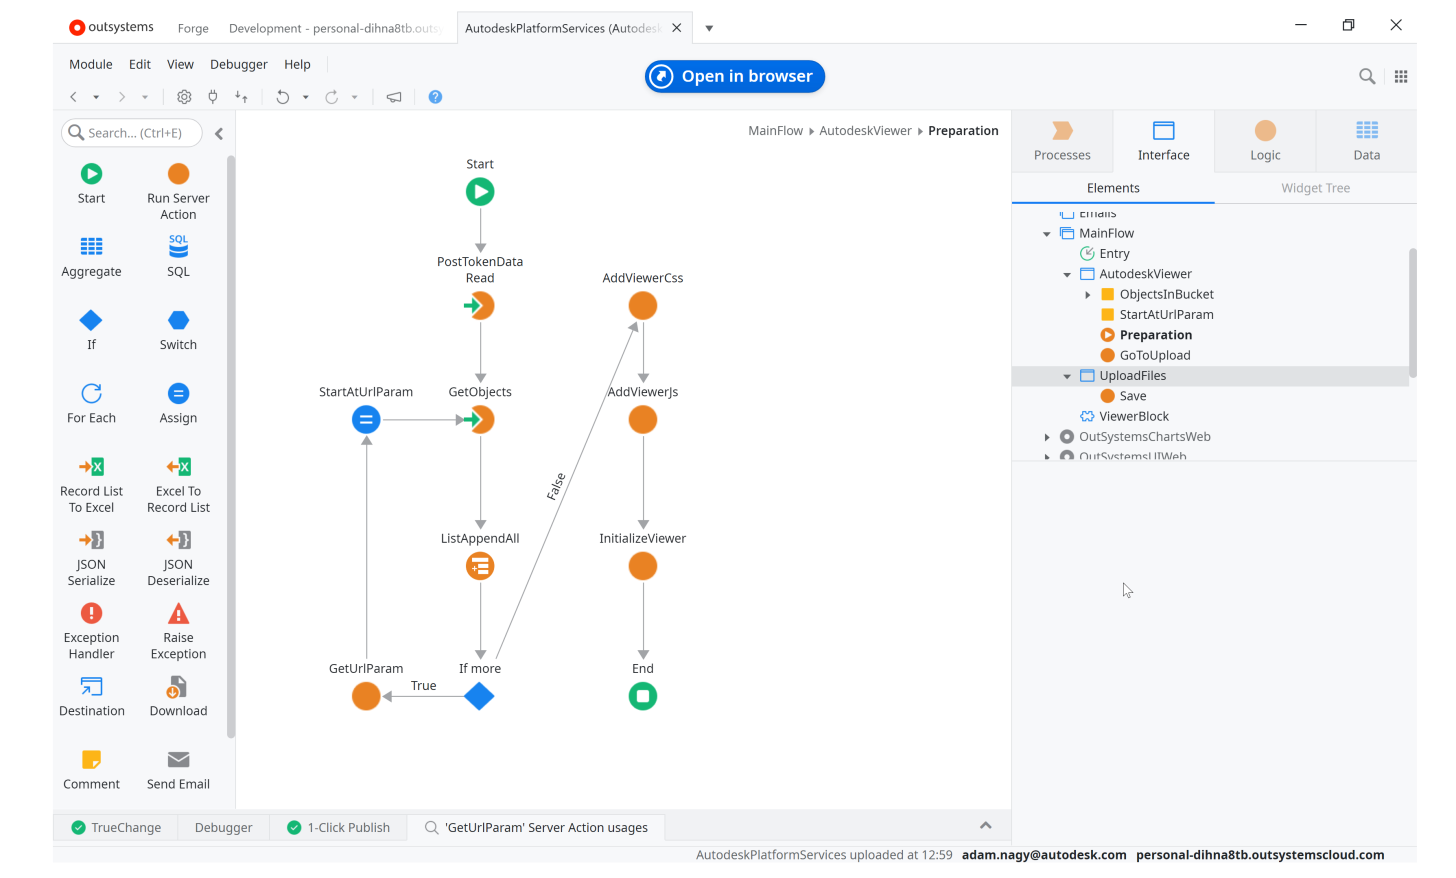
\includegraphics[width=15cm]{Figures/outsystems.png}
    \caption{Interface OutSystems}
    \label{fig:my_label} %Optional (If you want to reference the figure in later chapters)
\end{figure}

\begin{itemize}

    \item \textbf{OutSystems} propose des capacités d'intégration robustes avec divers systèmes bancaires, des systèmes existants et des applications tierces, permettant un flux de données et une interopérabilité transparents. La plateforme offre également des fonctionnalités de sécurité de niveau entreprise, notamment la gestion des identités, le chiffrement et la conformité aux normes du secteur telles que le RGPD et le PCI-DSS. Conçu pour l'évolutivité, OutSystems garantit que les solutions bancaires puissent croître en fonction des besoins de l'institution. Ses outils de création d'interfaces utilisateur riches et réactives améliorent l'expérience client sur les plateformes web et mobiles. Les applications développées à l'aide d'OutSystems incluent des processus d'intégration numérique simplifiés, des flux de traitement et d'approbation de prêts automatisés, ainsi que des applications bancaires mobiles riches en fonctionnalités.



          \begin{figure}[H]
              \centering
              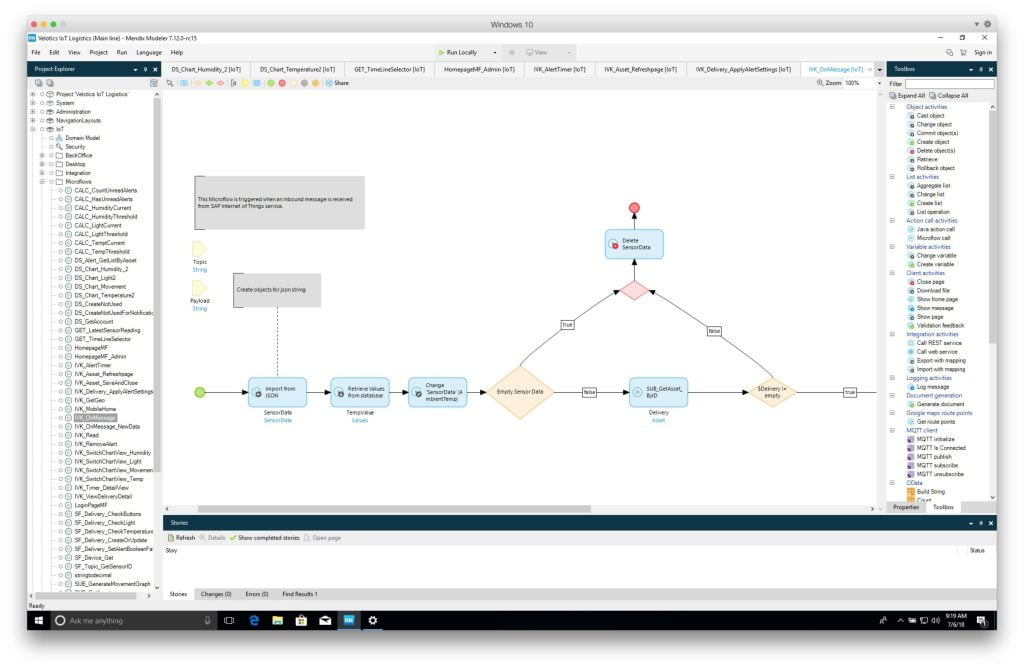
\includegraphics[width=15cm]{Figures/mendix.jpg}
              \caption{Interface Mendix}
              \label{fig:my_label} %Optional (If you want to reference the figure in later chapters)
          \end{figure}


    \item \textbf{Mendix} se concentre sur le développement piloté par modèle, permettant aux utilisateurs de créer des applications à l'aide de modèles visuels. Cela facilite la participation des analystes métier et des non-développeurs au processus de développement. Mendix propose des outils de collaboration complets qui favorisent la coopération entre les équipes informatiques et commerciales, garantissant ainsi que les applications répondent aux exigences de l'entreprise. Grâce à son développement piloté par l'IA, Mendix suggère des bonnes pratiques et optimise les performances des applications. La plateforme fournit également des connecteurs et des API prédéfinis pour l'intégration avec les systèmes bancaires centraux, les plateformes CRM et d'autres applications d'entreprise. Les applications construites avec Mendix incluent des solutions CRM personnalisées adaptées aux besoins spécifiques des banques, des applications de conformité réglementaire pour KYC (Know Your Customer) et AML (Anti-Money Laundering), et des flux de travail internes pour les pistes d'audit, la gestion des risques et les rapports financiers.



          \begin{figure}[H]
              \centering
              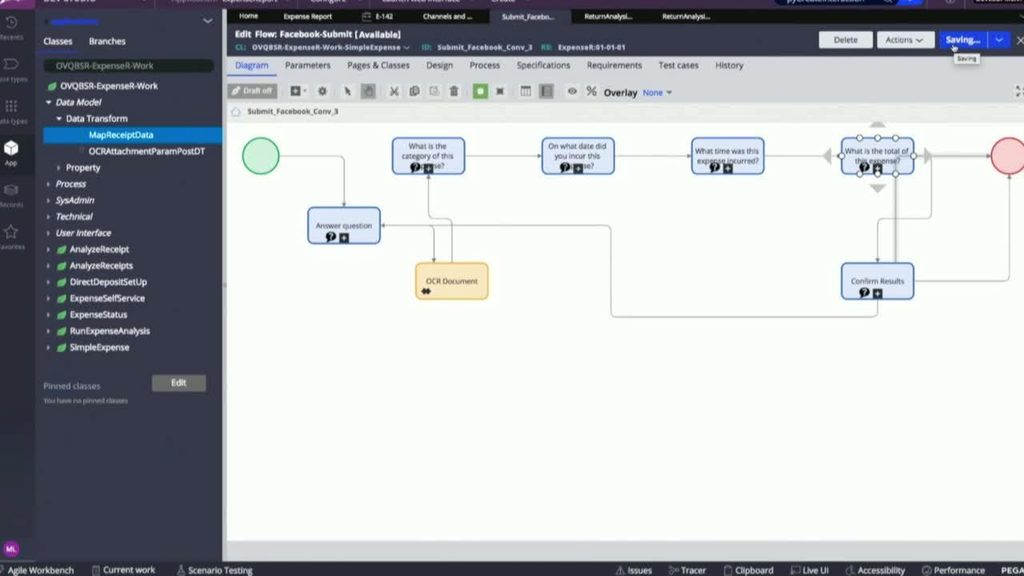
\includegraphics[width=15cm]{Figures/pega.jpg}
              \caption{Interface Pega}
              \label{fig:my_label} %Optional (If you want to reference the figure in later chapters)
          \end{figure}

    \item \textbf{Pega} est reconnu pour ses puissantes fonctionnalités de BPM (Business Process Management) et d'engagement client. Il aide les banques à automatiser les workflows et à gérer plus efficacement les interactions clients. La plateforme Pega intègre une prise de décision pilotée par l'IA, ce qui permet d'améliorer la personnalisation des services proposés aux clients. Les applications développées avec Pega incluent des processus d'intégration client automatisés, des assistants virtuels intelligents pour les demandes des clients et une gestion dynamique des cas pour traiter les demandes et les problèmes clients complexes.


          \begin{figure}[H]
              \centering
              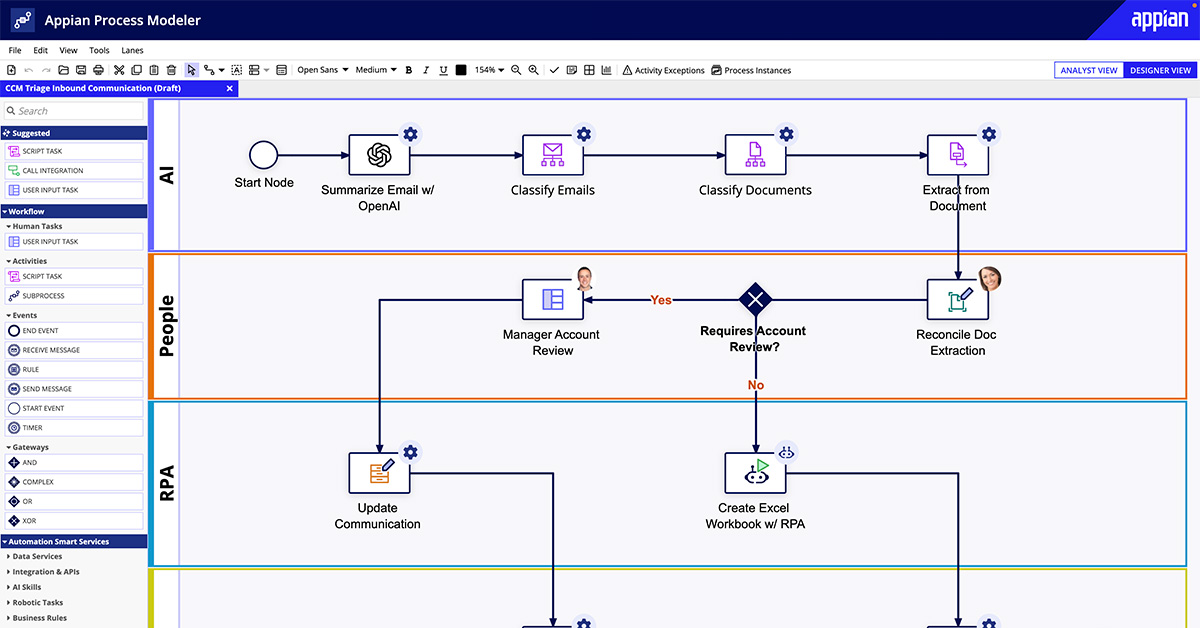
\includegraphics[width=15cm]{Figures/appian.jpg}
              \caption{Interface Appian}
              \label{fig:my_label} %Optional (If you want to reference the figure in later chapters)
          \end{figure}


    \item \textbf{Appian} est une autre plateforme low-code puissante, particulièrement axée sur la gestion des processus métier (BPM). Elle permet aux banques d'automatiser et d'optimiser des processus complexes, en s'intégrant aux outils d'automatisation robotisée des processus (RPA) pour réduire les efforts manuels et les erreurs. Les capacités avancées de gestion des données d'Appian offrent une vue unifiée des données clients, permettant une meilleure prise de décision. Ses outils de gestion de cas améliorent la prestation de services et la satisfaction client. Les applications développées à l'aide d'Appian incluent des systèmes de détection de fraude en temps réel basés sur l'apprentissage automatique et l'analyse, des améliorations du service client telles que des chatbots et des centres de service, ainsi que des solutions de gestion des risques garantissant la conformité aux exigences réglementaires.
\end{itemize}



En résumé, les plateformes low-code révolutionnent le paysage du développement logiciel dans de nombreux secteurs. En permettant le développement et le déploiement rapides d'applications, ces plateformes donnent aux organisations les moyens d'innover et de s'adapter rapidement à l'évolution du paysage numérique. Des plateformes comme OutSystems, Mendix, Appian et Pega se démarquent, mais d'autres acteurs importants existent également dans l'espace low-code, tels que Zoho Creator, Betty Blocks, Quick Base, Kissflow et Bubble. Ces plateformes offrent des fonctionnalités et des capacités diverses qui répondent à un large éventail de besoins opérationnels, de l'automatisation des workflows à l'amélioration de l'engagement client, en passant par l'augmentation de la productivité et la garantie de conformité.  Globalement, les plateformes low-code démocratisent le développement d'applications, le rendant accessible à un public plus large et accélérant considérablement le processus de transformation numérique pour de nombreuses organisations.

\subsection{Content Management System (CMS)}


\hspace{\parindent}Les systèmes de gestion de contenu (CMS) sont des outils essentiels pour gérer, créer et modifier du contenu numérique. Ces systèmes sont devenus indispensables pour les entreprises de toutes tailles, permettant une gestion efficace des sites web, blogs et autres plateformes numériques sans nécessiter de connaissances techniques approfondies.

Un CMS est une application logicielle qui permet aux utilisateurs de créer, éditer, organiser et publier du contenu numérique. Il fournit une interface conviviale pour gérer le contenu web et prend souvent en charge plusieurs utilisateurs dans un environnement collaboratif. L'objectif principal d'un CMS est de simplifier le processus de création de contenu, permettant ainsi aux utilisateurs non techniques de contribuer et de gérer efficacement le contenu numérique.

\textbf{A. Importance des CMS}

Les systèmes de gestion de contenu (CMS) simplifient la gestion du contenu numérique au sein d'une organisation, garantissant une présence en ligne constante et efficace. Les avantages clés incluent :

\begin{itemize}
    \item \textbf{Facilité d'utilisation}: La majorité des CMS disposent d'interfaces conviviales permettant la création et la manipulation de contenu sans connaissances en HTML, CSS ou tout autre langage de programmation utilisé dans le design web.

    \item \textbf{Collaboration}: Ils permettent la collaboration de plusieurs utilisateurs. Des rôles peuvent être créés et assignés, certains utilisateurs ayant plus d'accès et de permissions que d'autres.


    \item \textbf{Efficacité}: En consolidant la gestion du contenu, ils réduisent le temps et les efforts nécessaires pour maintenir les sites web et autres formes de contenu numérique.

    \item \textbf{Scalabilité}: Grâce à leur architecture flexible, ils peuvent gérer un volume important de contenu et de trafic, ce qui les rend adaptés aux entreprises de toutes tailles.

    \item \textbf{Optimisation SEO}: La plupart des plateformes CMS intègrent des outils et plugins tiers pour aider à l'optimisation du contenu pour les moteurs de recherche, augmentant ainsi la visibilité et le classement du contenu.
\end{itemize}

\textbf{B. Fonctionnalités des CMS}


Les plateformes CMS offrent une gamme de fonctionnalités visant à simplifier la gestion du contenu et à améliorer la fonctionnalité :


\begin{itemize}
    \item \textbf{Éditeur WYSIWYG}: Un éditeur \textit{"What You See Is What You Get"} permet aux utilisateurs de créer et formater du contenu avec une interface visuelle affichant l'apparence finale du contenu sur le site web.

    \item \textbf{Templates et Thèmes}: Ils proposent une variété de templates et thèmes préconçus, personnalisables pour correspondre à l'image de marque et au style de l'organisation.

    \item \textbf{Plugins et Extensions}: Ces modules complémentaires étendent la fonctionnalité du CMS, permettant des fonctionnalités telles que le commerce électronique, l'intégration aux réseaux sociaux et l'analyse.

    \item \textbf{Planification du Contenu}: Les utilisateurs peuvent programmer la publication de contenu à des moments précis, facilitant la planification et la gestion des publications.
    \item \textbf{Media Management}: Ils offrent des outils pour télécharger, organiser et gérer les fichiers multimédias tels que les images, vidéos et documents.

    \item \textbf{Gestion des Utilisateurs}: Ils prennent en charge le contrôle d'accès basé sur les rôles, permettant aux administrateurs de gérer les permissions et les niveaux d'accès des utilisateurs.
\end{itemize}

\textbf{C. Exemples et Applications}

Les CMS (Systèmes de Gestion de Contenu) sont largement employés dans divers secteurs, chacun présentant des besoins et des applications spécifiques. Parmi les exemples populaires, on trouve WordPress, Drupal, Joomla et SITECORE.
\begin{figure}[H]
    \centering
    
\includegraphics[width=6cm]{Figures/WordPress.png}
    \caption{WordPress logo}
    \label{fig:my_label} %Optional (If you want to reference the figure in later chapters)
\end{figure}

\begin{itemize}

    \item \textbf{WordPress} est l'un des systèmes de gestion de contenu (SGC) les plus populaires, reconnu pour son interface conviviale, sa vaste bibliothèque de thèmes et de plugins, et son solide support communautaire. Il convient à une large gamme d'applications, des blogs et sites web personnels aux sites d'entreprise et aux plateformes e-commerce.  La simplicité d'utilisation de WordPress pour le référencement (SEO) et sa flexibilité en font un choix de premier plan pour de nombreuses organisations.
          \\
          \\
          \begin{figure}[H]
              \centering
              
\includegraphics[width=5cm]{Figures/Drupal.png}
              \caption{Drupal logo}
              \label{fig:my_label} %Optional (If you want to reference the figure in later chapters)
          \end{figure}


    \item \textbf{Drupal} est un autre système de gestion de contenu (SGC), plébiscité pour sa haute personnalisation, sa scalabilité et ses fonctionnalités de sécurité robustes. Il est fréquemment utilisé par les agences gouvernementales, les institutions d'enseignement et les grands sites communautaires. Le support multilingue intégré de Drupal et ses mesures de sécurité solides en font un choix fiable pour les sites web complexes et à fort trafic.

          \begin{figure}[H]
              \centering
              
\includegraphics[width=7cm]{Figures/Joomla.png}
              \caption{Joomla logo}
              \label{fig:my_label} %Optional (If you want to reference the figure in later chapters)
          \end{figure}


    \item \textbf{Joomla} se positionne comme un juste milieu entre la convivialité et la fonctionnalité avancée. Il propose une large gamme d'extensions et de modèles, prend en charge plusieurs langues et bénéficie d'une communauté de développeurs active. Joomla convient parfaitement aux petites et moyennes entreprises, aux sites e-commerce et aux plateformes de réseaux sociaux.

          \begin{figure}[H]
              \centering
              
\includegraphics[width=5cm]{Figures/Sitecore.png}
              \caption{Sitecore logo }
              \label{fig:my_label} %Optional (If you want to reference the figure in later chapters)
          \end{figure}


    \item \textbf{Sitecore} se démarque par ses outils avancés de gestion de l'expérience client, son intégration transparente avec d'autres systèmes d'entreprise, ses analyses complètes et sa scalabilité. Il est couramment utilisé par les grandes entreprises pour gérer un contenu volumineux et offrir des expériences utilisateur personnalisées. L'intégration de Sitecore avec les outils marketing et sa prise en charge des sites e-commerce complexes en font une solution robuste pour les grandes organisations.

\end{itemize}
\hspace{\parindent}Malgré tous les avantages qu'elles offrent, les plateformes CMS présentent également certains inconvénients. En voici quelques-uns : limitations de la personnalisation, risques de sécurité, problèmes de performance liés aux gros volumes de contenu, et nécessité d'une maintenance et de mises à jour régulières. Les organisations doivent donc tenir compte de ces facteurs lors du choix d'un CMS.

L'avenir des plateformes CMS sera très probablement marqué par l'intégration de l'intelligence artificielle et du machine learning pour améliorer la personnalisation et l'optimisation du contenu. On assistera également à un intérêt accru pour les CMS headless, qui séparent le système de gestion de contenu du back-end de la couche de présentation du front-end, permettant une gestion plus précise de la distribution du contenu sur des plateformes disparates.

Par conséquent, les outils CMS tels que WordPress, Drupal, Joomla, Sitecore et autres sont essentiels pour la gestion de contenu. Ils permettent aux organisations de disposer d'une plateforme en ligne performante, d'interagir avec leur audience et d'évoluer dans l'environnement numérique en constante mutation. Ces plateformes continueront à se développer à mesure des avancées technologiques afin de fournir aux utilisateurs plus de fonctionnalités et de faciliter la gestion du contenu, tout en offrant une meilleure expérience utilisateur.

% \subsection{BPMN}

% \hspace{\parindent}BPMN, ou Business Process Model and Notation (en français, Modélisation et Notation des Processus d'Entreprise), est une méthode standardisée de modélisation graphique des processus d'entreprise. Il offre un moyen complet de cartographier les différentes activités, événements et décisions au sein d'un processus métier, ce qui facilite la compréhension et l'analyse de ces processus par les parties prenantes. BPMN est largement utilisé dans divers secteurs pour améliorer l'efficacité, rationaliser les opérations et garantir la cohérence dans la gestion des processus métier.

% C'est une représentation visuelle permettant de spécifier les processus d'entreprise dans un modèle de processus métier. Il est conçu pour être facilement compréhensible par toutes les parties prenantes de l'entreprise, y compris les analystes métier, qui créent et affinent les processus, les développeurs techniques, responsables de la mise en œuvre des processus et les chefs d'entreprise, qui supervisent et gèrent les processus.

% BPMN utilise un ensemble de symboles normalisés pour représenter les différents aspects d'un processus métier. Ces symboles se répartissent en plusieurs catégories :
% \\
% \begin{figure}[H] 
%     \centering
%     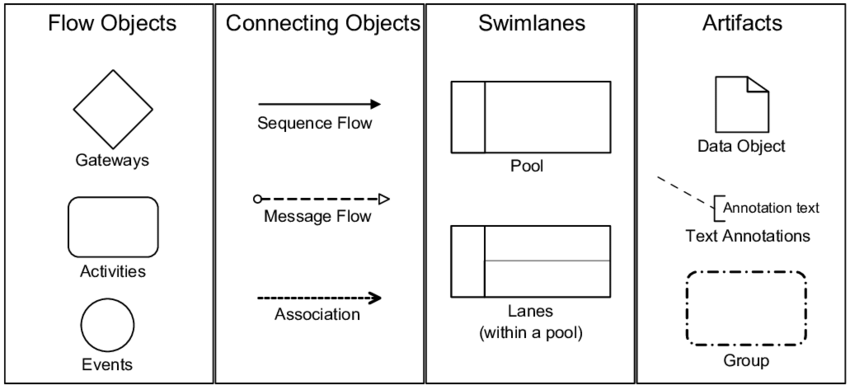
\includegraphics[width=15cm]{Figures/BPMN.png}
%     \caption{BPMN Core Elements of Process diagram}
%     \label{fig:my_label} %Optional (If you want to reference the figure in later chapters)
% \end{figure}

% \\

% \begin{itemize}
% \item \textbf{Flow Objects} 
%     \begin{itemize}
%       \item \textbf{Events} : Represent things that happen (start, intermediate, and end events).
%       \item \textbf{Activities} : Work or tasks performed (tasks, sub-processes).
%       \item \textbf{Gateways} : Decision points that determine the flow of the process (e.g., exclusive, parallel).
%     \end{itemize}

% \item \textbf{Connecting Objects} 
%     \begin{itemize}
%       \item \textbf{Sequence Flows}: Show the order of activities.
%       \item \textbf{Message Flows}: Represent the flow of messages between separate process participants.
%       \item \textbf{Associations}: Link artifacts and text to flow objects.
%     \end{itemize}

% \item \textbf{Swimlanes} 
%     \begin{itemize}
%       \item \textbf{Pools}: Represent major participants in the process.
%       \item \textbf{Lanes}: Sub-divisions within pools that organize and categorize activities.
%     \end{itemize}

% \item \textbf{Artifacts} 
%     \begin{itemize}
%       \item \textbf{Data Objects}: Represent data required or produced by activities.
%       \item \textbf{Groups}: Used to group elements of a diagram informally.
%       \item \textbf{Annotations}: Provide additional information about the process.
%     \end{itemize}

% \end{itemize}


% \hspace{\parindent}BPMN is a crucial tool for businesses aiming to document, analyze, and enhance their processes. By offering a standardized and visual representation, it facilitates better communication, deeper understanding, and continuous improvement across diverse sectors. As organizations embrace digital transformation, it will remain integral to effective process management. In the following sections, we will delve into the various BPMN symbols in detail and examine their application in Fawri-Flows, demonstrating the practical use of this powerful notation system.



\subsection{Présentation de Fawri-Flow}


\hspace{\parindent}Fawri-Flow est un outil de Gestion Intelligente des Processus Métier (IBPM) associé à un moteur de rendu frontal d'écrans. Il permet la transformation et la digitalisation efficaces de divers types de processus, tout en offrant un niveau élevé de personnalisation en termes de design et d'expérience utilisateur (UX).

Fawri-Flow permet d'adapter dynamiquement tout changement ad hoc dans le modèle ou la procédure en modifiant le schéma du processus ou le formulaire de chaque nœud du processus.

La conception des flux de travail repose principalement sur des nœuds de divers types, chacun étant attribué à un rôle spécifique ou suivant une matrice d'approbation configurable :

\begin{itemize}
    \item \textbf{Tâche utilisateur}: Il s'agit d'une page de formulaire ou d'un ensemble de pages attribuées à un rôle spécifique (par exemple : utilisateur final ou agent de traitement).

    \item \textbf{Tâches système ou connecteur}: Permettent l'exécution fluide d'un script grâce à l'éditeur intelligent de la solution.
    \item \textbf{Passerelles}: Ces éléments permettent au dossier ou à la demande de suivre un ou plusieurs chemins en fonction d'un ensemble de conditions entièrement paramétrables, basées sur les données fournies par l'utilisateur ou calculées par le système.
\end{itemize}

Fawri-Flow dispose également d'un Flow Designer, un module d'automatisation des processus dans un environnement de conception graphique. Il permet aux propriétaires de processus d'utiliser le langage naturel pour automatiser les approbations, les tâches, les notifications et les opérations d'enregistrement sans nécessiter de codage.

Flow Designer offre plusieurs avantages : il consolide diverses capacités d'automatisation dans une seule interface, permettant ainsi aux utilisateurs de visualiser et de gérer les processus métier de manière intuitive. Il fournit des descriptions en langage naturel pour faciliter la compréhension des non-techniciens et favorise l'automatisation en permettant aux experts métier de créer et partager des actions réutilisables, ce qui réduit les coûts de développement et de mise à niveau.

\begin{figure}[H]
    \centering
    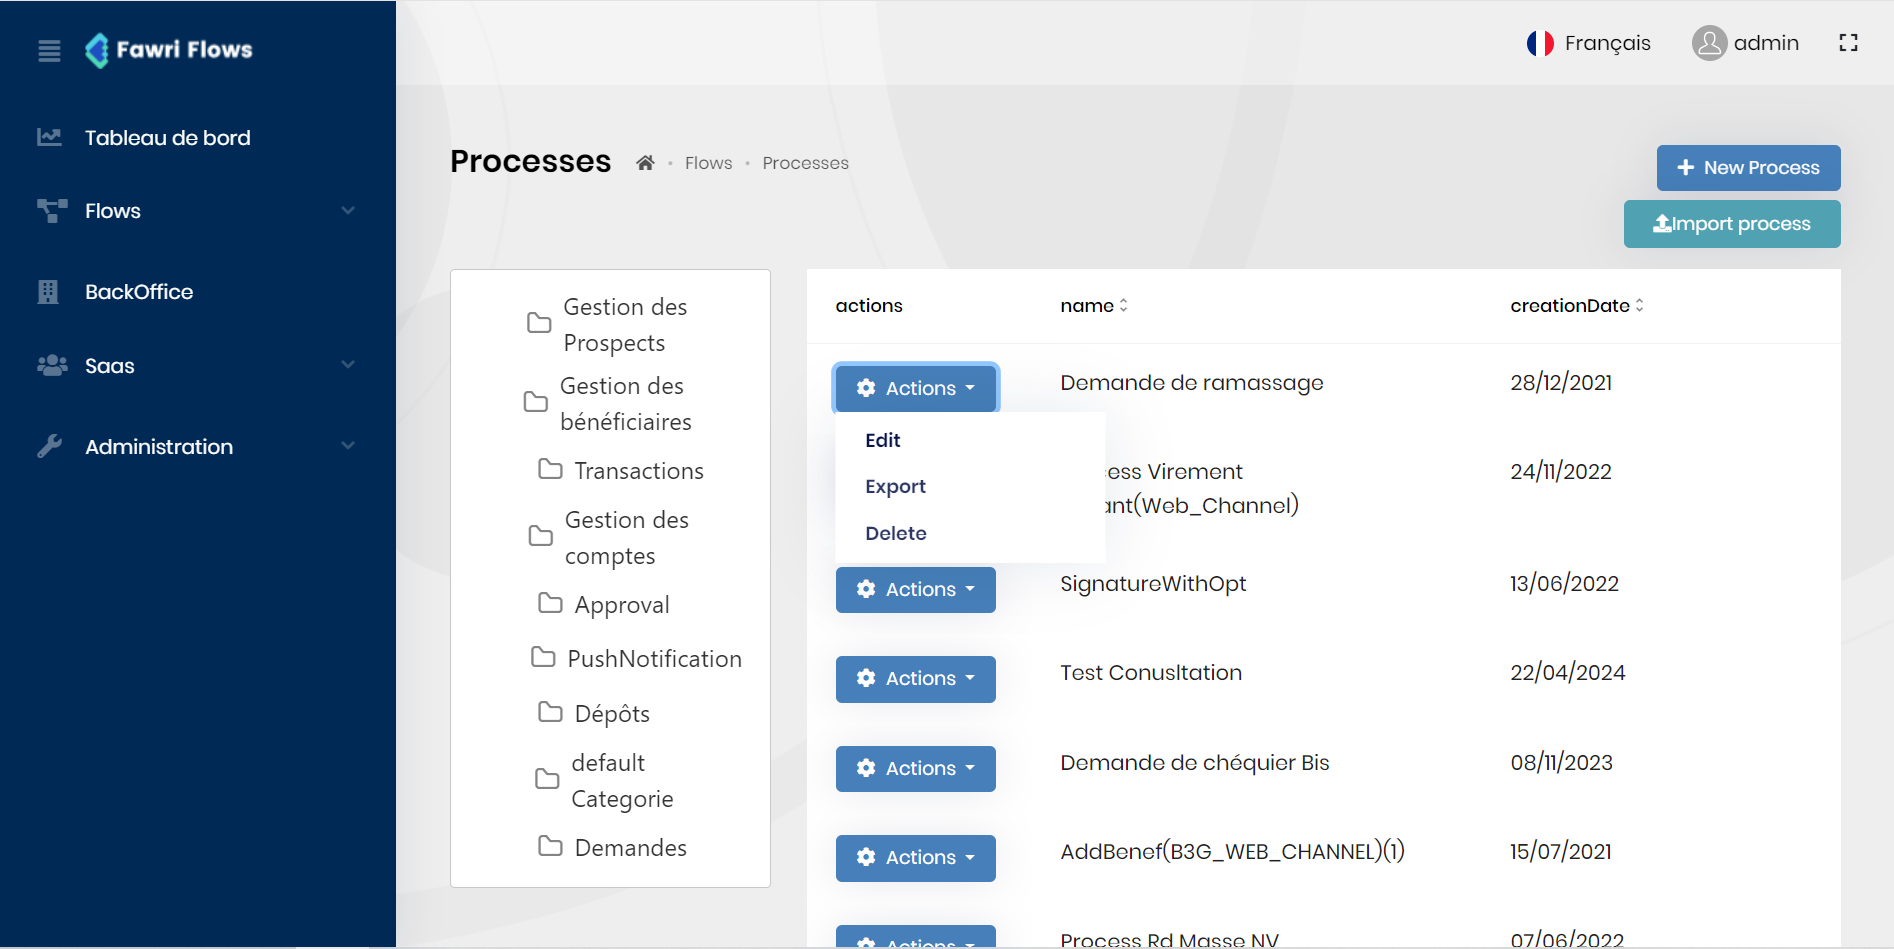
\includegraphics[width=15cm]{Figures/processmanagement.png}
    \caption{Gestion des processus avec Fawri-Flows}
    \label{fig:my_label} %Optional (If you want to reference the figure in later chapters)
\end{figure}



\section{Problématique }

\hspace{\parindent}Bien que Fawri-Flow permette la création de processus intégrables et réutilisables, son intégration actuelle exige une manipulation directe du code. Cette approche engendre d'importantes inefficacités dans le développement des applications clientes, nécessitant des efforts manuels pour coder des composants spécifiques. Cela non seulement consomme davantage de temps et de ressources, mais limite également la capacité à réutiliser efficacement les fonctionnalités existantes et à les adapter aux besoins évolutifs des applications. En outre, en dehors de l'intégration des processus, le développement complet de l'application pour chaque client doit être réalisé. Cette dépendance à la programmation manuelle des composants entrave le processus de développement, compromettant ainsi la productivité et la rentabilité du projet.

Face à cette situation, se pose la question suivante : \textbf{Comment évoluer vers une solution low-code qui simplifie le processus de développement d'applications, en exploitant pleinement les capacités de Fawri-Flow, tout en éliminant le besoin de manipulation directe du code ?}

\section{Objectifs du Projet et Solutions Proposées}

\hspace{\parindent}B3G a voulu lancer \textbf{Fawri-CMS}, une nouvelle solution alignée sur la tendance du "low-code". L'objectif principal de ce projet est de simplifier considérablement le processus de développement des applications clientes, notamment dans les secteurs du \textit{digital banking} et des portefeuilles numériques, en éliminant la nécessité de recourir à la programmation traditionnelle. Avec une interface conviviale de type "drag and drop", Fawri-CMS facilitera également l'intégration des processus métier élaborés avec Fawri-Flows.

Ce nouvel outil vise plusieurs objectifs stratégiques. Tout d'abord, il cherche à réduire drastiquement le temps et les ressources nécessaires au développement des applications, en supprimant la phase de codage manuel pour chaque fonctionnalité. En rendant possible la création d'applications professionnelles et fonctionnelles même pour un public non spécialisé en programmation, Fawri-CMS aspire à démocratiser l'accès au développement d'applications. De plus, il entend améliorer l'efficacité opérationnelle des entreprises en facilitant une intégration fluide des processus métier dans les applications clientes, même sans compétences techniques approfondies. Enfin, en libérant les développeurs des contraintes techniques, Fawri-CMS encourage l'innovation et la créativité, en les incitant à se concentrer sur la conception et l'expérience utilisateur.




\section{Gestion du projet}

\subsection{Approche Scrum}

\hspace{\parindent}Dans le choix de la méthodologie pour ce projet, plusieurs facteurs ont influencé notre décision, notamment les exigences spécifiques du projet, sa nature et ses objectifs. La méthodologie Scrum s'est imposée comme le cadre le plus adapté pour répondre à ces besoins. Voici les principaux éléments de Scrum :

\textbf{Rôles :}


\begin{itemize}
    \item \textbf{Product Owner} : Responsable de définir et prioriser le backlog du produit, déterminer les fonctionnalités à développer et garantir la valeur du produit.

    \item \textbf{Scrum Master} : Facilitateur du processus Scrum, s'assurant que l'équipe respecte les principes et pratiques de Scrum et résout les obstacles éventuels.

    \item \textbf{Équipe de développement} : Groupe de personnes responsables de réaliser les fonctionnalités du produit. Dans le cadre de ce projet, nous faisons partie de cette équipe et sommes responsables de sa réalisation.
\end{itemize}



\textbf{Artéfacts :}


\begin{itemize}
    \item \textbf{Product Backlog} : Liste ordonnée des fonctionnalités à développer, représentant les besoins et exigences du produit.

    \item \textbf{Sprint Backlog} :Liste des fonctionnalités sélectionnées à partir du Product Backlog pour être développées lors d'un sprint spécifique.

    \item \textbf{Increment} : Version fonctionnelle du produit résultant des fonctionnalités développées pendant un sprint.
\end{itemize}


\textbf{Événements :}


\begin{itemize}
    \item \textbf{Sprint} : Période de temps définie (généralement de 1 à 4 semaines) au cours de laquelle l'équipe de développement crée un incrément de produit.

    \item \textbf{Sprint Planning} : Réunion de planification où l'équipe sélectionne les fonctionnalités à développer pendant le sprint et détermine comment les réaliser.

    \item \textbf{Daily Scrum} : Réunion quotidienne de l'équipe pour partager les progrès, synchroniser les activités et discuter des obstacles éventuels.

    \item \textbf{Sprint Review} : Réunion à la fin du sprint pour présenter l'incrément du produit aux parties prenantes et recueillir des commentaires.

    \item \textbf{Sprint Retrospective} : Réunion pour réfléchir sur le sprint écoulé, identifier les points forts et les améliorations possibles, et adapter les pratiques.


\end{itemize}


La nature itérative et incrémentielle de Scrum correspondait parfaitement à la volonté d'optimiser la gestion du projet et la collaboration au sein de notre équipe. Face à un projet dynamique et évolutif tel que celui-ci, Scrum offrait la flexibilité nécessaire pour s'adapter aux changements tout en garantissant des livraisons régulières de fonctionnalités.

De plus, la structure claire des rôles, des artefacts et des événements de Scrum nous permettait de définir des responsabilités précises et de favoriser la transparence tout au long du processus de développement. Cette clarté était essentielle pour assurer une communication efficace au sein de l'équipe et avec les parties prenantes externes.

En adoptant Scrum, nous avons pu bénéficier d'une approche collaborative et adaptative, permettant à notre équipe de rester focalisée sur la valeur à apporter au produit tout en s'assurant d'une progression constante. La méthodologie Scrum a ainsi joué un rôle crucial dans le succès de notre projet, en fournissant un cadre solide pour la gestion de projet agile et en favorisant la collaboration, la responsabilisation et l'amélioration continue.


\begin{figure}[H]
    \centering
    
\includegraphics[width=4cm]{Figures/scrum.png}
    \caption{Scrum logo}
    %\label{fig:my_label} %Optional (If you want to reference the figure in later chapters)
\end{figure}








\subsection{Outils de collaboration}

\hspace{\parindent}Pour améliorer l'efficacité et la productivité au sein de l'équipe B3G, l'intégration d'outils collaboratifs s'est avérée indispensable. Nous nous sommes concentrés sur deux outils déjà en usage avant le début du stage : \textbf{Microsoft Teams} et \textbf{Outlook}. Microsoft Teams est devenu un élément central de notre collaboration. En créant des espaces de travail dédiés à chaque projet ou équipe, nous avons pu regrouper les discussions, les partages de fichiers et les réunions, facilitant ainsi une communication fluide et une organisation optimale des tâches.

Les fonctionnalités de chat, d'appels audio et vidéo de Teams ont été d'une grande utilité pour maintenir une communication efficace et instantanée, quel que soit l'emplacement géographique des membres de l'équipe. De plus, les partages d'écran se sont avérés particulièrement utiles lors des réunions pour présenter des informations clés ou réaliser des démonstrations.\\

\begin{figure}[H]
    \centering
    
\includegraphics[width=6cm]{Figures/Microsoft_Teams.png}
    \caption{Microsoft Teams logo}
    %\label{fig:my_label} %Optional (If you want to reference the figure in later chapters)
\end{figure}


Outlook, de son côté, a été utilisé pour la gestion des calendriers et la planification. Nous avons pu créer des rendez-vous, des réunions et des rappels directement dans Outlook, ce qui nous a permis de structurer nos emplois du temps et d'éviter les conflits d'horaire. Grâce à la fonction de partage de calendrier, nous avons pu visualiser les disponibilités des membres de l'équipe et planifier des réunions aux moments les plus propices. De plus, la fonction d'intégration d'Outlook avec d'autres outils, tels que Teams, nous a facilité la transformation des e-mails en discussions collaboratives, ce qui a favorisé une communication améliorée et une productivité accrue.
\\
\\
\begin{figure}[H]
    \centering
    
\includegraphics[width=6cm]{Figures/outlook.png}
    \caption{Microsoft Oulook logo}
    %\label{fig:my_label} %Optional (If you want to reference the figure in later chapters)
\end{figure}



\subsection{Gestion des versions}

Puisque nous adhérons à la méthodologie agile, une collaboration étroite entre les membres de l'équipe sur le code est cruciale pour garantir la transparence du développement et le succès du projet. C'est pourquoi le choix d'une plateforme de gestion de code adaptée à nos besoins revêtait une importance capitale.

Dans cette optique, notre société a opté pour \textbf{Azure DevOps Server}. Cette plateforme de développement logiciel offre un ensemble complet d'outils pour la collaboration, le suivi des problèmes, la gestion des versions et le déploiement continu. Elle permet à notre équipe de travailler de manière synchronisée et efficace, en mettant l'accent sur la transparence et la qualité du code.
\\
\\
\begin{figure}[H]
    \centering
    
\includegraphics[width=8cm]{Figures/azur.png}
    \caption{Microsoft Azur DevOps logo}
    %\label{fig:my_label} %Optional (If you want to reference the figure in later chapters)
\end{figure}


\subsection{Planning du projet}

\hspace{\parindent}Dans ce projet, nous avons adopté la planification par sprint avec Scrum, qui fait partie de la méthodologie agile. Cette approche repose sur des cycles itératifs et incrémentaux appelés sprints, généralement d'une durée de 2 à 4 semaines. Elle offre une visualisation claire et pratique des actions planifiées, permettant de suivre et de contrôler le déroulement de chaque étape du projet. Ce diagramme représente graphiquement les tâches et leur durée. Pour ce projet de fin d’études, la figure suivante présente la planification par sprints, offrant une vue d'ensemble de la planification anticipée des tâches. Grâce à cette visualisation, nous pouvons gérer efficacement les échéances et assurer le bon déroulement du projet en respectant les délais fixés.

\begin{figure}[H]
    \centering
    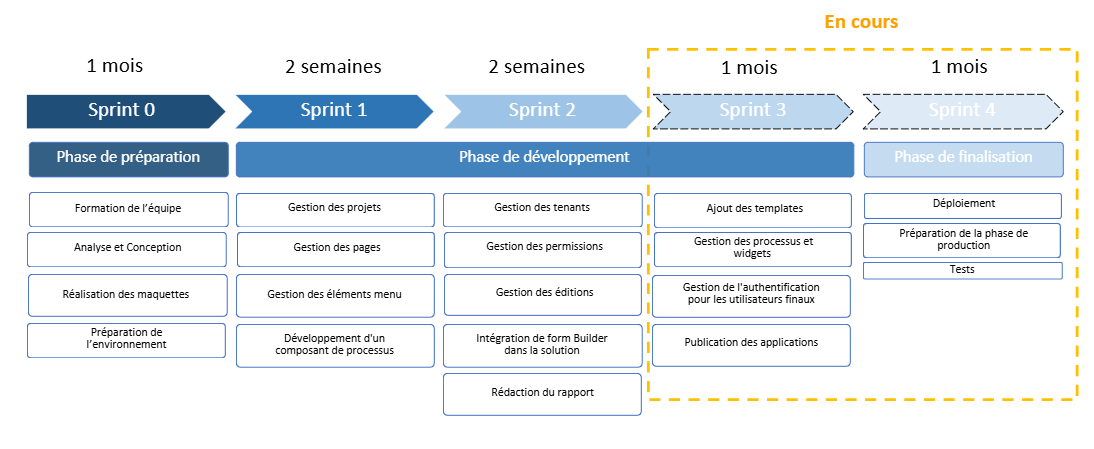
\includegraphics[width=18cm]{Figures/sprints.PNG}
    \caption{Planning du Projet par Sprints}
    %\label{fig:my_label} %Optional (If you want to reference the figure in later chapters)
\end{figure}



\newpage

\section*{Conclusion}

\hspace{\parindent}Dans ce chapitre, nous avons commencé par présenter B3G, une entreprise spécialisée dans le développement de solutions digitales pour le secteur bancaire, en mettant en avant ses produits et sa clientèle. Ensuite, nous avons examiné le contexte global de notre projet, mettant en évidence l'importance croissante de la transformation digitale, ainsi que des concepts clés tels que la technologie "Low-Code", les systèmes de gestion de contenu (CMS), et notre produit Fawri-Flow. Nous avons ensuite défini clairement la problématique de notre projet, suivi par la définition de ses objectifs et des solutions proposées. Nous avons également décrit en détail notre approche méthodologique basée sur Scrum, les outils de collaboration et de gestion des versions utilisés, ainsi que la planification prévisionnelle du projet.



\chapter{Analyse et Conception}
\label{chap:Analysis and Design}
\section*{Introduction}

\hspace{\parindent}Cette partie du rapport vise à offrir une vision approfondie et détaillée de l'analyse et de la conception du projet, et à mettre en lumière les choix stratégiques, les décisions clés et les résultats obtenus. Elle constitue une base solide pour la mise en œuvre et le développement futurs du projet. Nous entamons par une analyse fonctionnelle, suivie d'une étude approfondie des besoins, comprenant l'identification des parties prenantes, la collecte des exigences fonctionnelles et la modélisation des processus métier. Ensuite, nous réalisons la conception du système en détaillant l'architecture globale et les différents composants qui le constituent.
\pagebreak







\section{Analyse des besoins}
\subsection{Identification des acteurs}

\hspace{\parindent}Les acteurs, qui représentent des rôles spécifiques joués par les utilisateurs, interagissent avec notre système en tant qu'entités internes ou externes. Ces acteurs peuvent consulter ou modifier l'état du système en envoyant et en recevant des messages contenant des données. Les différents acteurs impliqués dans notre système sont détaillés dans le tableau suivant.


\begin{table}[h]
  \centering
  \captionsetup{justification=centering}
  \begin{tabular}{|p{0.2\textwidth}|p{0.2\textwidth}|p{0.5\textwidth}|}
    \hline
    \textbf{Acteur}            & \textbf{Rôle}                                & \textbf{Responsabilités}                                                                                                                                                                                                \\ \hline
    \textbf{Super Admin}       & Gestion complète du système                  & Personnel de B3G ayant des privilèges étendus pour gérer les tenants et éditions, les projets (menus et pages), la gestion de contenu (widgets et processus), ainsi que la gestion des utilisateurs et les permissions. \\ \hline
    \textbf{Tenant Admin}      & Administration d'un tenant spécifique        & Clients de B3G ayant des privilèges administratifs pour gérer les projets, la gestion de contenu, les utilisateurs et les autorisations au sein de leur propre espace de travail (tenant).                              \\ \hline
    \textbf{Utilisateur final} & Consultation des projets/applications créés. & Personne ou entité qui utilise les plateformes créées par un tenant pour accéder aux fonctionnalités, contenus et services proposés.                                                                                    \\ \hline
  \end{tabular}
  \caption{Liste des acteurs}
  \label{tab:actors}
\end{table}

\textbf{NB} : "Tenant" dans ce contexte se réfère à une instance spécifique de l'application, souvent déployée pour un client ou une organisation spécifique. Chaque tenant fonctionne comme une entité indépendante, avec ses propres données, configurations et utilisateurs.

\subsection{Besoins fonctionnels}

\hspace{\parindent} Les besoins fonctionnels décrivent les fonctionnalités et les services essentiels que notre système doit offrir pour satisfaire les attentes des utilisateurs et des parties prenantes. Voici les besoins fonctionnels identifiés pour notre projet :

\begin{itemize}
  \item \textbf{Gestion des utilisateurs :}\\
        Authentification et autorisation, chaque acteur doit obligatoirement s'authentifier avant d'interagir avec le système.Ainsi que le système doit gérer les permissions en fonction des rôles des utilisateurs (Super Admin, Tenant Admin, Utilisateur Final).


        Les Super Admins et les Tenant Admins doivent pouvoir créer, modifier et supprimer des comptes utilisateurs.

  \item \textbf{Gestion des tenants :}\\
        Pour la création et configuration des tenants, Les Super Admins doivent pouvoir créer et configurer de nouveaux tenants. Ainsi que les Tenant Admins doivent pouvoir configurer les paramètres de leur propre tenant, notamment les préférences et les règles spécifiques.

        Quant à la gestion des données et des configurations, chaque tenant doit disposer de ses propres données et configurations isolées des autres tenants pour garantir la sécurité et la confidentialité.

  \item \textbf{Gestion des projets et du contenu :}\\
        Les Tenant Admins doivent pouvoir créer, modifier et supprimer des projets au sein de leur tenant.

        Les projets doivent pouvoir être configurés avec des menus, des pages et des widgets spécifiques selon les besoins du tenant.

        Les Tenant Admins doivent pouvoir ajouter, éditer et supprimer du contenu dans les projets, y compris les widgets et les processus.

        Organisation et structuration du contenu pour une navigation efficace et intuitive pour les utilisateurs finaux.

  \item \textbf{Gestion des autorisations :}\\
        Les Super Admins doivent pouvoir définir des autorisations pour les différents rôles au niveau global.

        Les Tenant Admins doivent pouvoir définir des autorisations spécifiques pour les utilisateurs au sein de leur tenant, en fonction des projets et des contenus.

        Le système doit permettre de contrôler les droits d'accès, de modification et de suppression pour chaque utilisateur ou groupe d'utilisateurs en fonction de leur rôle et des autorisations définies.

  \item \textbf{Gestion des éditions :}\\
        Les Super Admins doivent pouvoir créer et configurer différentes éditions du système, adaptées à des besoins spécifiques ou à des types de clients particuliers.

        Les Super Admins doivent pouvoir personnaliser chaque édition en fonction des besoins des clients, y compris les fonctionnalités disponibles, les thèmes et les configurations spécifiques.

        Les Super Admins doivent pouvoir mettre à jour et maintenir les éditions, incluant l'application de nouvelles fonctionnalités, correctifs et améliorations spécifiques à chaque édition.

\end{itemize}



\subsection{Besoins non fonctionnels}

\hspace{\parindent}Les besoins non fonctionnels définissent les qualités et les contraintes auxquelles le système doit répondre pour garantir sa performance, sa sécurité et sa convivialité. Voici les principaux besoins non fonctionnels identifiés pour notre projet :
\begin{itemize}
  \item \textbf{Sécurité :}
        \begin{enumerate}
          \item Protection des données sensibles et conformité aux normes de sécurité.
          \item Cryptage des données et gestion des vulnérabilités.
        \end{enumerate}

  \item \textbf{Performance :}
        \begin{enumerate}
          \item Temps de réponse rapide et capacité à gérer une charge élevée.
          \item Optimisation des temps de chargement.
        \end{enumerate}

  \item \textbf{Disponibilité :}\\
        Garantir un temps de disponibilité élevé, visant à atteindre un taux cible de disponibilité de 90\%, et mettre en place des mécanismes de récupération pour assurer une continuité de service en cas de défaillance.

  \item \textbf{Facilité d'Utilisation :}
        \begin{enumerate}
          \item Interface utilisateur conviviale et documentation complète.

          \item Formation et support pour les utilisateurs.
        \end{enumerate}

  \item \textbf{Interopérabilité :}\\
        Capacité à intégrer avec d'autres systèmes et à échanger des données.
\end{itemize}






\section{Conception}

\hspace{\parindent}Maintenant que l'analyse a été finalisée, nous sommes prêts à passer à la phase de conception. Cette étape consiste à formaliser les besoins fonctionnels du projet en utilisant des diagrammes UML. Ces diagrammes permettent de représenter le comportement fonctionnel ainsi que la structure du système de manière claire et précise.

\subsection{Diagramme de cas d'utilisation global}

\hspace{\parindent}Le diagramme de cas d'utilisation, un composant essentiel des diagrammes UML de comportement, est utilisé pour illustrer le fonctionnement d'un système et saisir ses exigences. Il expose les fonctionnalités principales du système ainsi que son domaine d'application, tout en mettant en avant les interactions entre le système et les acteurs impliqués. Les cas d'utilisation et les acteurs figurant dans ces diagrammes décrivent les actions réalisées par le système et la manière dont les acteurs interagissent avec celui-ci, sans entrer dans les détails de son fonctionnement interne. Conformément à cette définition, la figure suivante présente le diagramme de cas d'utilisation global du système, mettant en scène trois acteurs : \textbf{le Super Admin, le Tenant Admin} et \textbf{l'Utilisateur final (End user)}, comme le montre le diagramme suivant :


%\textbf{-------Insert diag cas d'utilisation global---------}


\begin{figure}[H]
  \centering
  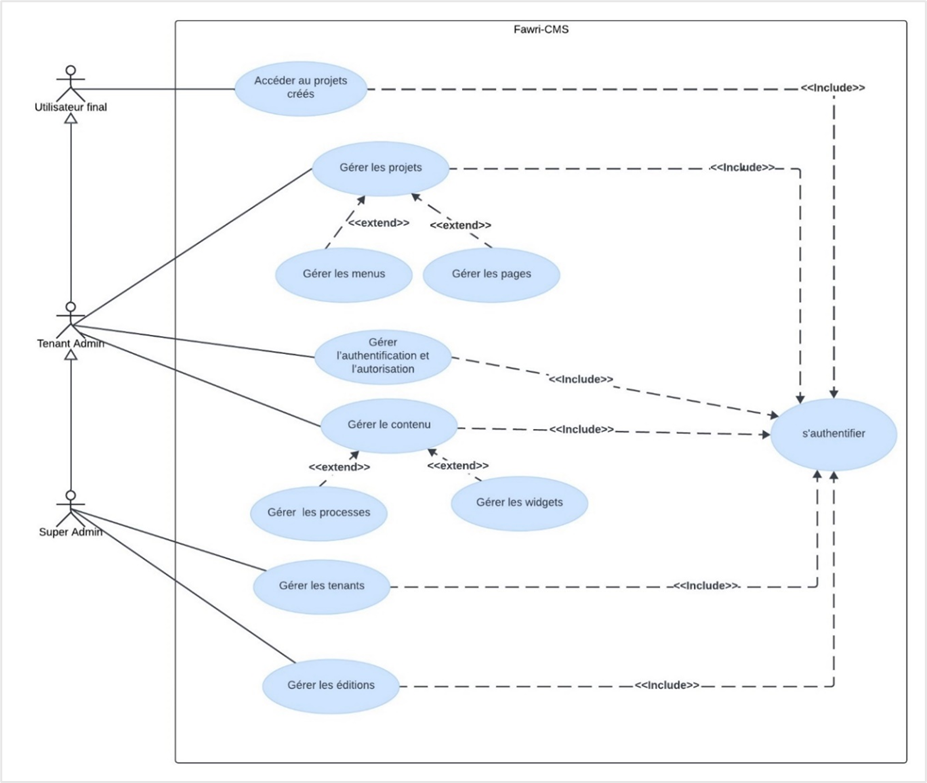
\includegraphics[width=17cm]{Figures/use case globale.png}
  \caption{Diagramme de cas d'utilisation global}
  %\label{fig:my_label} %Optional (If you want to reference the figure in later chapters)
\end{figure}





\subsection{Diagramme de cas d'utilisation : Gestion des projets}

\hspace{\parindent}Ce diagramme, figure \ref*{diag2}, détaille les cas d'utilisation pour la gestion des projets, incluant la gestion des pages et des menus. Il précise les fonctionnalités et les cas d'utilisation ainsi que les interactions avec les différents acteurs.

% \textbf{----------Insert diag cas d'utilisation gestion des projets-----------}


\begin{figure}[H]
  \centering
  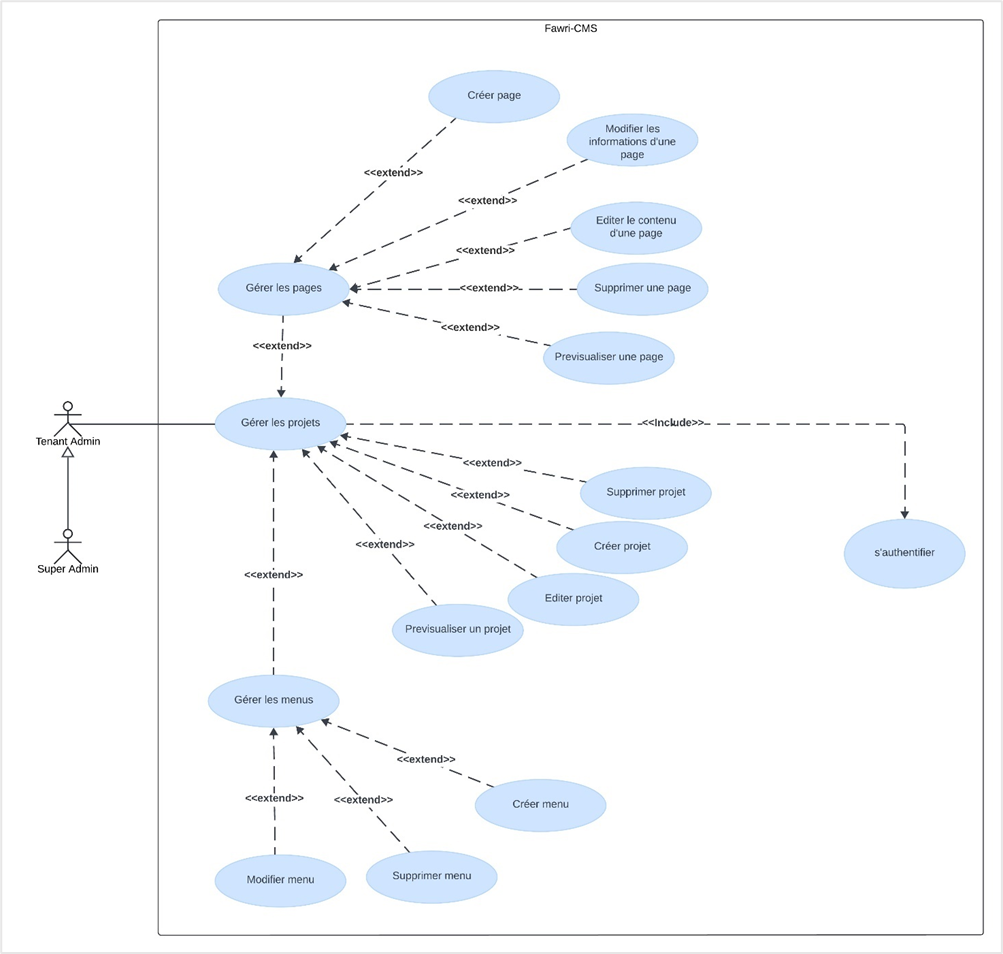
\includegraphics[width=17cm]{Figures/use case gestion des projets.png}
  \caption{Diagramme de cas d'utilisation : gestion des projets}
  \label{diag2} %Optional (If you want to reference the figure in later chapters)
\end{figure}



\subsection{Diagramme de cas d’utilisation : Gestion de contenu}
\hspace{\parindent}Dans cette partie, nous allons présenter un diagramme de cas d'utilisation qui détaille les différents aspects de la gestion de contenu au sein de notre système Fawri-CMS. Ce diagramme, figure \ref*{diag3}, met en lumière les principales fonctionnalités, telles que la gestion des widgets et des processus. Il illustre comment les acteurs, comme les super administrateurs et les administrateurs de tenants, interagissent avec le système pour créer, éditer, supprimer des widgets, et intégrer des processus dans les pages du CMS. Le diagramme suivant représente le diagramme de cas d'utilisation pour la gestion de contenu :

% \textbf{--------Insert diag cas d'utilisation Gestion de contenu--------}

\begin{figure}[H]
  \centering
  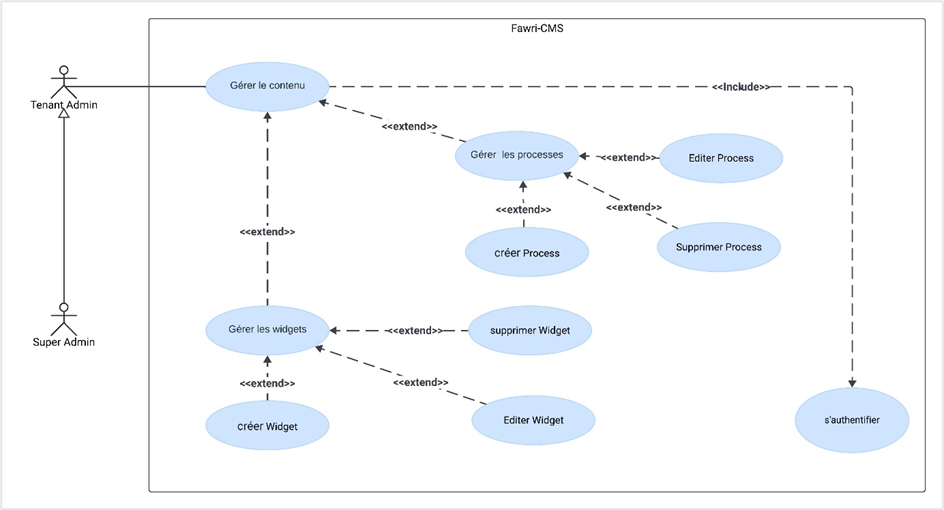
\includegraphics[width=17cm]{Figures/gestion de contenu.png}
  \caption{Diagramme de cas d'utilisation : gestion de contenu}
  \label{diag3} %Optional (If you want to reference the figure in later chapters)
\end{figure}



\subsection{Diagramme de cas d'utilisation : Gestion des tenants, éditions et permissions}

\hspace{\parindent}Dans cette partie, nous allons présenter un diagramme de cas d'utilisation qui détaille les différents aspects de la gestion des tenants, des éditions et des permissions au sein de notre système Fawri-CMS. Ce diagramme, comme le montre la figure \ref*{diag4}, met en lumière les principales fonctionnalités nécessaires à la gestion efficace des tenants, y compris la création, l'édition et la suppression des tenants, ainsi que la gestion des rôles et des permissions associés. Il illustre comment les acteurs, tels que les super administrateurs et les administrateurs de tenants, interagissent avec le système pour administrer ces aspects critiques du CMS.

Le diagramme suivant représente les cas d'utilisation pour la gestion des tenants, l'édition et les permissions dans notre système Fawri-CMS :
% \textbf{-----Insert diag cas d'utilisation Gestion des tenants, éditions et permissions----}

\begin{figure}[H]
  \centering
  \includegraphics[width=17cm]{Figures/Gestion des tenants éditions et permissions.png}
  \caption{Diagramme de cas d'utilisation : gestion des tenants, éditions et permissions}
  \label{diag4} %Optional (If you want to reference the figure in later chapters)
\end{figure}





\subsection{Diagramme de classes}
\hspace{\parindent}Dans cette partie, nous allons présenter le diagramme de classes de notre système Fawri-CMS. Ce diagramme offre une vue détaillée des classes du système ainsi que leurs relations. Il illustre comment les entités principales interagissent entre elles et comment les différentes fonctionnalités sont implémentées à travers ces interactions.

Le diagramme de classes met en évidence les attributs et les méthodes des classes, fournissant ainsi une vue structurelle de notre application. Il inclut des classes pour la gestion des projets, des pages, des menus, des widgets, des tenants et des permissions, montrant comment ces éléments s'intègrent pour fournir les fonctionnalités complètes du CMS.

Le diagramme suivant représente la structure des classes dans notre système Fawri-CMS :

% \textbf{---Insert diag cas de class----}


\begin{figure}[H]
  \centering
  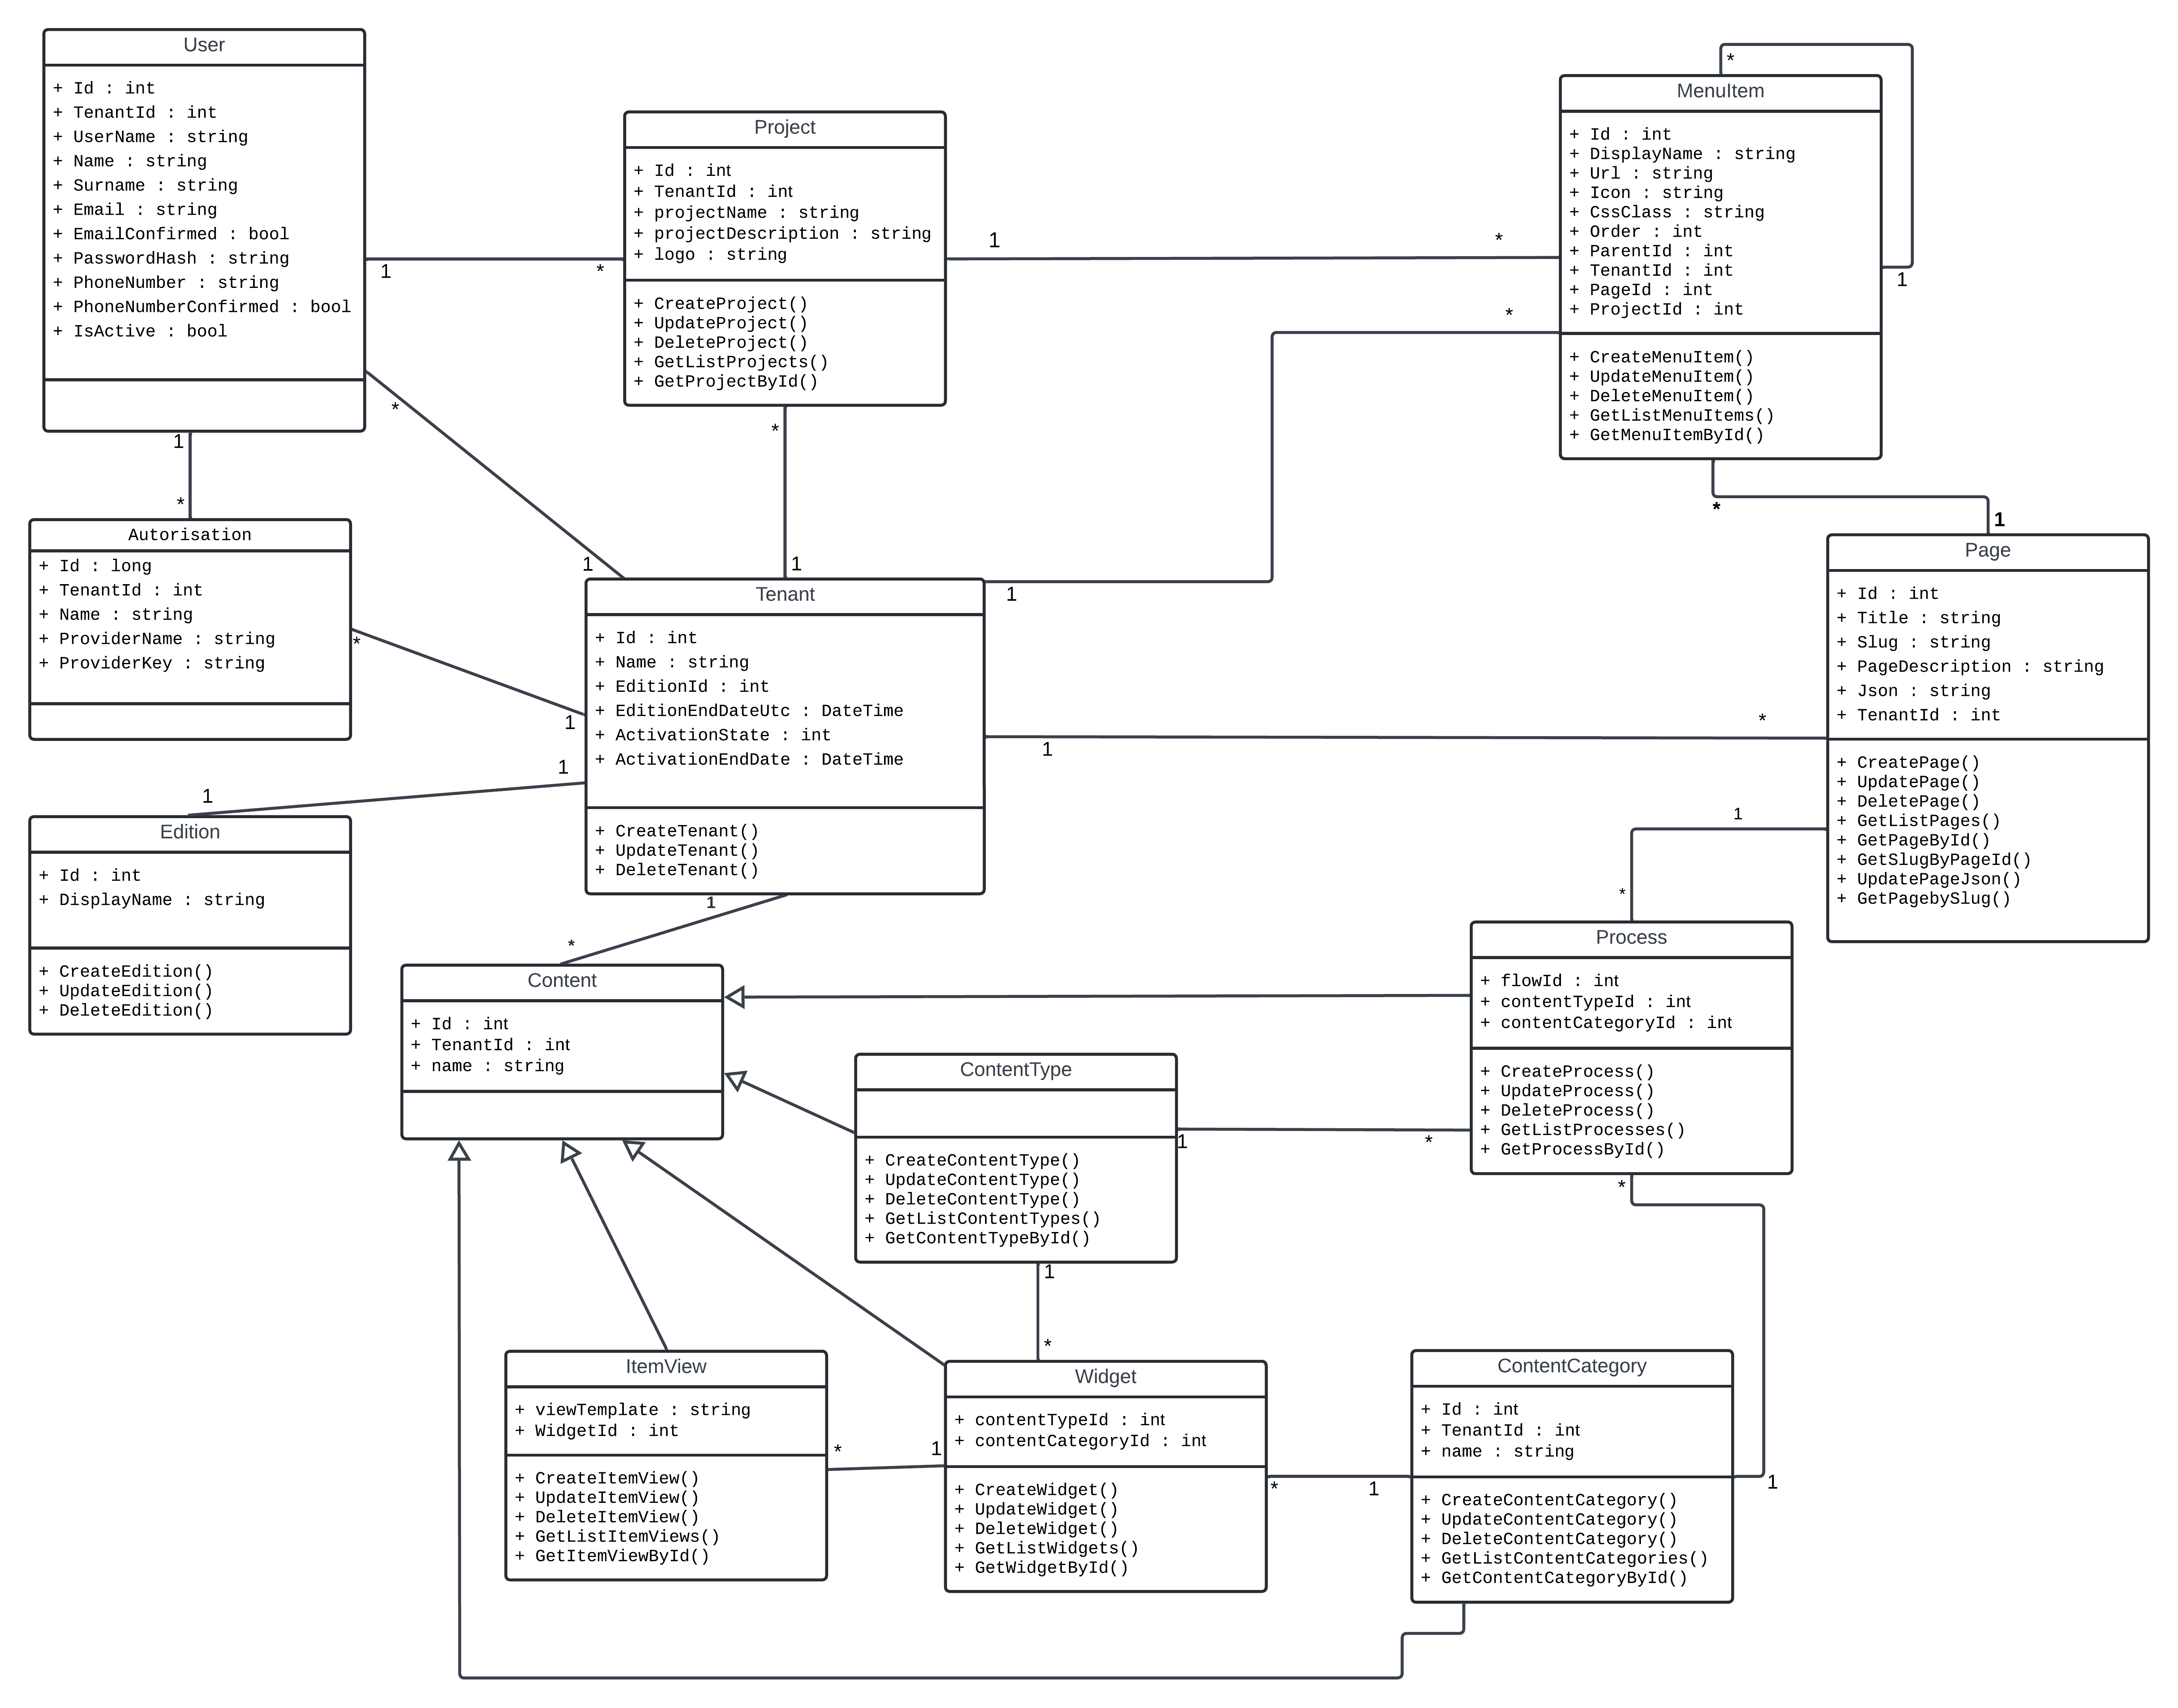
\includegraphics[width=20cm]{Figures/diag de classe.png}
  \caption{Diagramme de classes}
  %\label{fig:my_label} %Optional (If you want to reference the figure in later chapters)
\end{figure}




\textbf{User} : Représente les utilisateurs du système avec des informations générales et des mécanismes d'authentification.

\textbf{Autorisation} : Gère les autorisations et les rôles des utilisateurs dans le système.

\textbf{Project} : Gère les projets créés par les utilisateurs, y compris les opérations de création, mise à jour et suppression.

\textbf{MenuItem} : Représente les éléments de menu associés aux projets, permettant la navigation dans le système.

\textbf{Page} : Gère les pages de contenu au sein des projets, y compris leur création, mise à jour et suppression.

\textbf{Process} : Représente les processus associés aux contenus, gérant leur cycle de vie dans le système.

\textbf{Tenan}t : Gère les tenants, qui sont des instances spécifiques du système déployées pour différents clients ou organisations.

\textbf{Edition} : Gère les éditions du système, qui sont des versions personnalisées adaptées à des besoins spécifiques des clients.

\textbf{Content} : Gère le contenu au sein des tenants, permettant la création et l'organisation du contenu.

\textbf{ContentType} : Définit les types de contenu pouvant être créés et gérés dans le système.

\textbf{Widget} : Gère les widgets, qui sont des composants réutilisables dans les pages et projets.

\textbf{ContentCategory} : Organise les contenus en différentes catégories pour une meilleure gestion et structuration.

\textbf{ItemView} : Représente les vues d'éléments, définissant comment les widgets sont affichés dans le système.



\subsection{Diagrammes de séquence}

\begin{enumerate}

  \item Récupération de la liste des processus

        Le diagramme de séquence ci-dessous illustre le processus par lequel le tenant admin ou le super admin interagit avec Fawri-CMS pour récupérer la liste des processus disponibles depuis l'API Fawri-Flow. Ce diagramme décrit les échanges entre les différents acteurs et systèmes impliqués dans cette opération.

        % \textbf{-------insert Diagramme de séquence : Récupération de la liste des processus-------}

        \begin{figure}[H]
          \centering
          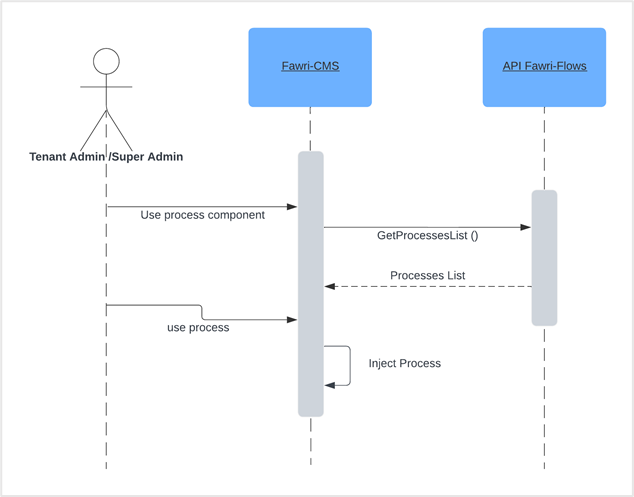
\includegraphics[width=11cm]{Figures/Diagramme_sequence _Recuperation_list_proc.png}
          \caption{Diagramme de séquence  Récupération de la liste des processus}
          %\label{fig:my_label} %Optional (If you want to reference the figure in later chapters)
        \end{figure}


  \item Gestion des projets\\
        Le diagramme de séquence ci-dessous montre le processus de gestion des projets au sein de Fawri-CMS. Il décrit les interactions entre le tenant admin/super admin, Fawri-CMS, et la base de données (DB) lors de la création et de la gestion des projets, les pages associées et les éléments de menu.
        % \\
        % \\
        % \textbf{-------insert Diagramme de séquence : Gestion des projets-------}
        % \\
        % \\
        \begin{figure}[H]
          \centering
          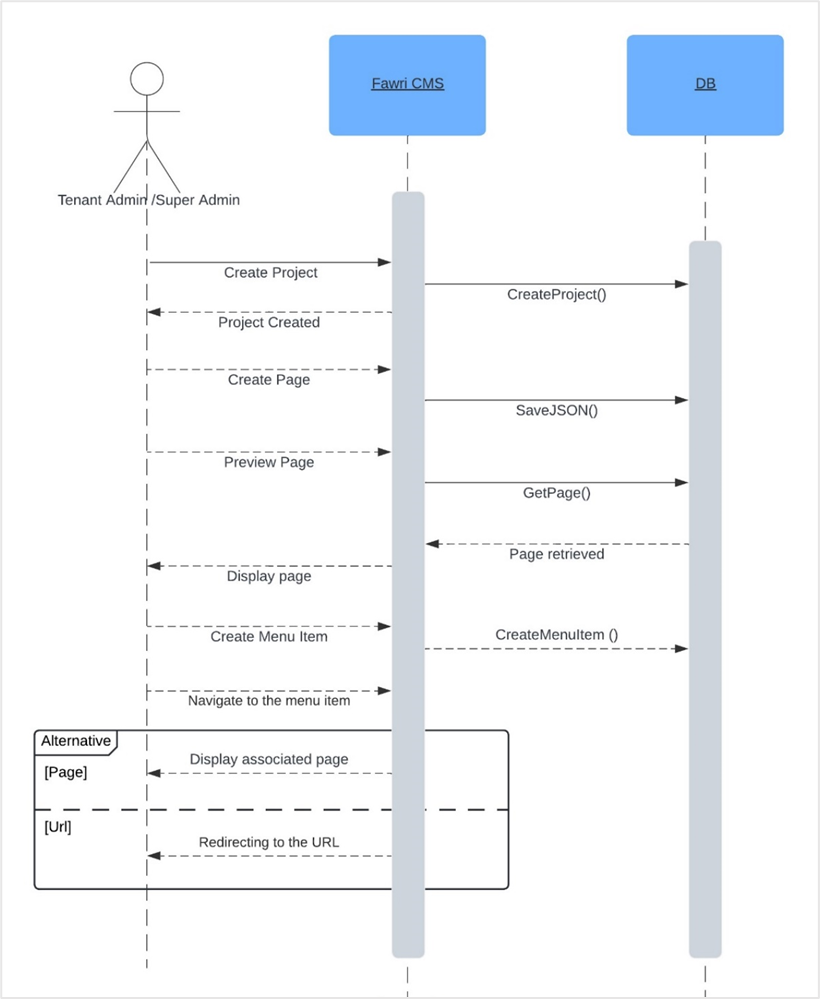
\includegraphics[width=11cm]{Figures/diagsec_Gestion_projets.png}
          \caption{Diagramme de séquence : gestion des projets}
          %\label{fig:my_label} %Optional (If you want to reference the figure in later chapters)
        \end{figure}




  \item Gestion des permissions
        \hspace{\parindent}Le diagramme de séquence ci-dessous illustre le processus de gestion des permissions dans Fawri-CMS. Il décrit les interactions entre le super admin/tenant admin, Fawri-CMS, et la base de données (DB) lors de la création de rôles, la gestion des permissions, la définition des autorisations, et l'ajout d'utilisateurs aux rôles.
        % \\
        % \\
        % \textbf{-------insert Diagramme de séquence : Gestion des permissions-------}
        % \\
        % \\
        \begin{figure}[H]
          \centering
          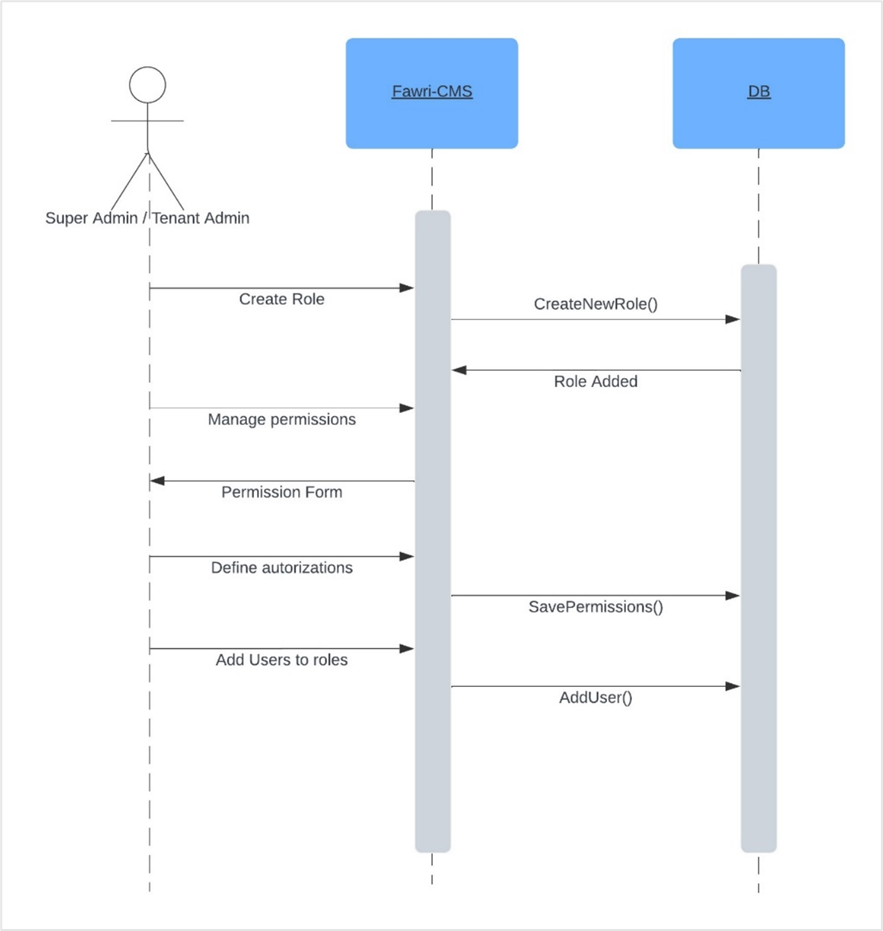
\includegraphics[width=11cm]{Figures/diagsec_Gestion_permissions.png}
          \caption{Diagramme de séquence : gestion des permissions}
          %\label{fig:my_label} %Optional (If you want to reference the figure in later chapters)
        \end{figure}



  \item Gestion des éditions et des tenants

        \hspace{\parindent}Ce diagramme de séquence illustre le processus de gestion des éditions et des tenants dans Fawri-CMS. Il décompose les interactions entre le super administrateur, Fawri-CMS et la base de données (DB) en étapes claires et concises, couvrant les actions de création d'éditions, de gestion des tenants.
        % \\
        % \\
        % \textbf{-------insert Diagramme de séquence : Gestion des éditions et des tenants-------}
        % \\
        % \\

        \begin{figure}[H]
          \centering
          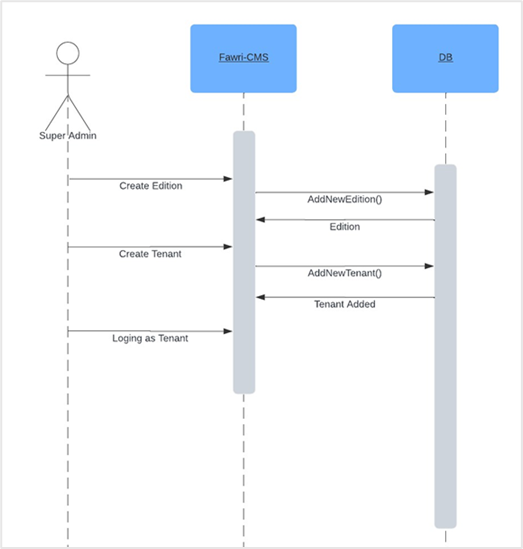
\includegraphics[width=11cm]{Figures/diagsec_Gestion_editions_tenants.png}
          \caption{Diagramme de séquence : gestion des éditions et des tenants}
          %\label{fig:my_label} %Optional (If you want to reference the figure in later chapters)
        \end{figure}

        % \item Gestion des éditions, des tenants et des projets
        Le diagramme d'activité ci-dessous illustre le processus de gestion des éditions, des tenants et des projets au sein de Fawri-CMS.
        % \\
        % \\
        % \textbf{-------insert Diagramme-------}
        % \\
        % \\




        % \item Diagramme d'activité : Gestion des Permissions
        %       \hspace{\parindent}Le diagramme d'activité ci-dessous illustre le processus de gestion des permissions au sein de Fawri-CMS. Il décrit les étapes et les décisions prises par le super admin/tenant admin pour créer, modifier et gérer les permissions des utilisateurs, des rôles, et les autorisations associées.
        %       \\
        %       \\
        %       \textbf{-------insert Diagramme-------}
        %       \\
        %       \\

\end{enumerate}




\section{Charte Graphique}

\hspace{\parindent}La charte graphique est essentielle pour garantir une identité visuelle cohérente et professionnelle à travers toutes les interfaces et supports du projet Fawri-CMS. Elle définit les règles de présentation visuelle et les standards à respecter pour tous les éléments graphiques de l'application.

\subsection{Logo et Identité Visuelle :}

\hspace{\parindent}Le logo, figure \ref*{logocms} doit être utilisé dans toutes les communications officielles et sur toutes les pages de l'application. Il est crucial pour l'identité de la marque.

\textbf{Format} : SVG ou PNG pour assurer une haute qualité et une adaptabilité.

\textbf{Utilisation} : En-têtes de page, pieds de page, documents marketing et matériel de présentation. Il doit être placé de manière cohérente, généralement en haut à gauche de chaque page.
\\
\begin{figure}[H]
  \centering
  
\includegraphics[width=6cm]{Figures/fawri_cms_logo.PNG}
  \caption{Logo Fawri CMS}
  \label{logocms} %Optional (If you want to reference the figure in later chapters)
\end{figure}


\subsection{Palette de couleurs}
\hspace{\parindent}Les couleurs jouent un rôle crucial dans l'identité visuelle de Fawri-CMS. Dans notre projet, nous avons utilisé la palette de couleurs suivante :
\\
\begin{figure}[H]
  \centering
  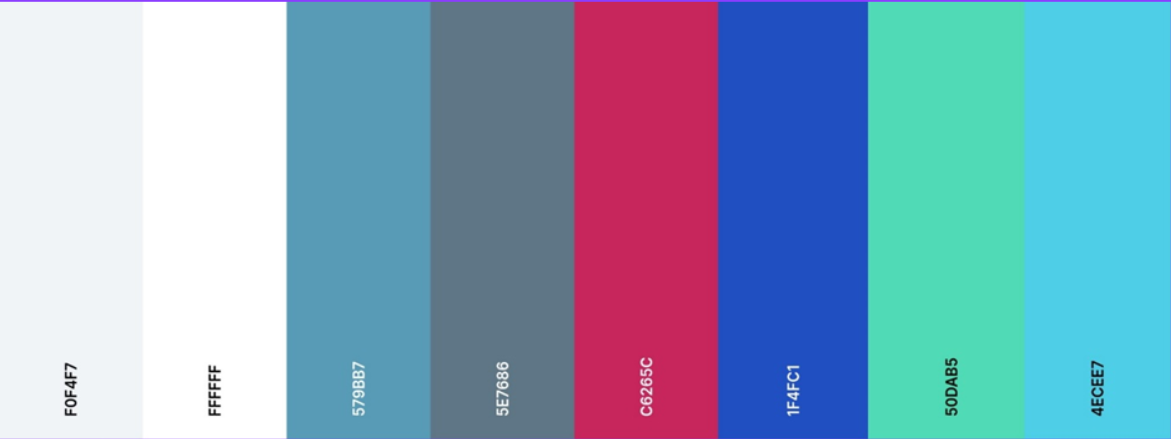
\includegraphics[width=12cm]{Figures/palette.PNG}
  \caption{La palette des couleurs}
  %\label{fig:my_label} %Optional (If you want to reference the figure in later chapters)
\end{figure}



\subsection{Typographie}
\hspace{\parindent}La typographie contribue à la lisibilité et à la cohérence visuelle de l'application Fawri-CMS.

\textbf{Police principale} : Sans-serif

La police principale est principalement utilisée pour les titres et les sous-titres, apportant une distinction claire entre les sections. Elle est également employée dans le corps du texte, les menus, les boutons, ainsi que dans les cellules des tableaux.

\begin{itemize}
  \item Titre 1 (h1) : 20 px

  \item Menu Items : 14 px

  \item Titre des colonnes : 14 px

  \item Contenu des tables : 14 px

  \item Texte du bouton : 14 px
\end{itemize}










\subsection{Boutons et Interactions}
\hspace{\parindent}Dans le cadre de notre projet Fawri-CMS, les boutons et les éléments interactifs doivent être clairement définis et facilement identifiables par les utilisateurs. Une attention particulière est accordée à leur conception pour garantir une expérience utilisateur optimale. Cela inclut l'utilisation de couleurs distinctes, de tailles appropriées et de styles cohérents pour tous les boutons et éléments interactifs afin de s'assurer qu'ils se démarquent visuellement et sont intuitivement reconnaissables pour les utilisateurs finaux.

\textbf{Boutons primaires :}
\begin{itemize}
  \item Couleur de fond : Bleu (\#1F4FC1)

  \item Texte : Blanc (\#FFFFFF)

  \item Bordure : 2px arrondie
\end{itemize}

\textbf{Boutons secondaires :}
\begin{itemize}
  \item Couleur de fond : (\#FFFFFF)

  \item Texte : Shadow Blue (\#5E7686)

  \item Bordure Solide Shadow Blue (\#5E7686)
\end{itemize}

\textbf{Boutons d'alerte}
\begin{itemize}
  \item Couleur de fond : Rouge (\#FF3300)

  \item Texte : Blanc (\#FFFFFF)

  \item Bordure : 2px arrondie
\end{itemize}










\subsection{Icônes}
\hspace{\parindent}Dans ce projet, nous avons utilisé la bibliothèque d'icônes Font Awesome.
\\
\begin{figure}[H]
  \centering
  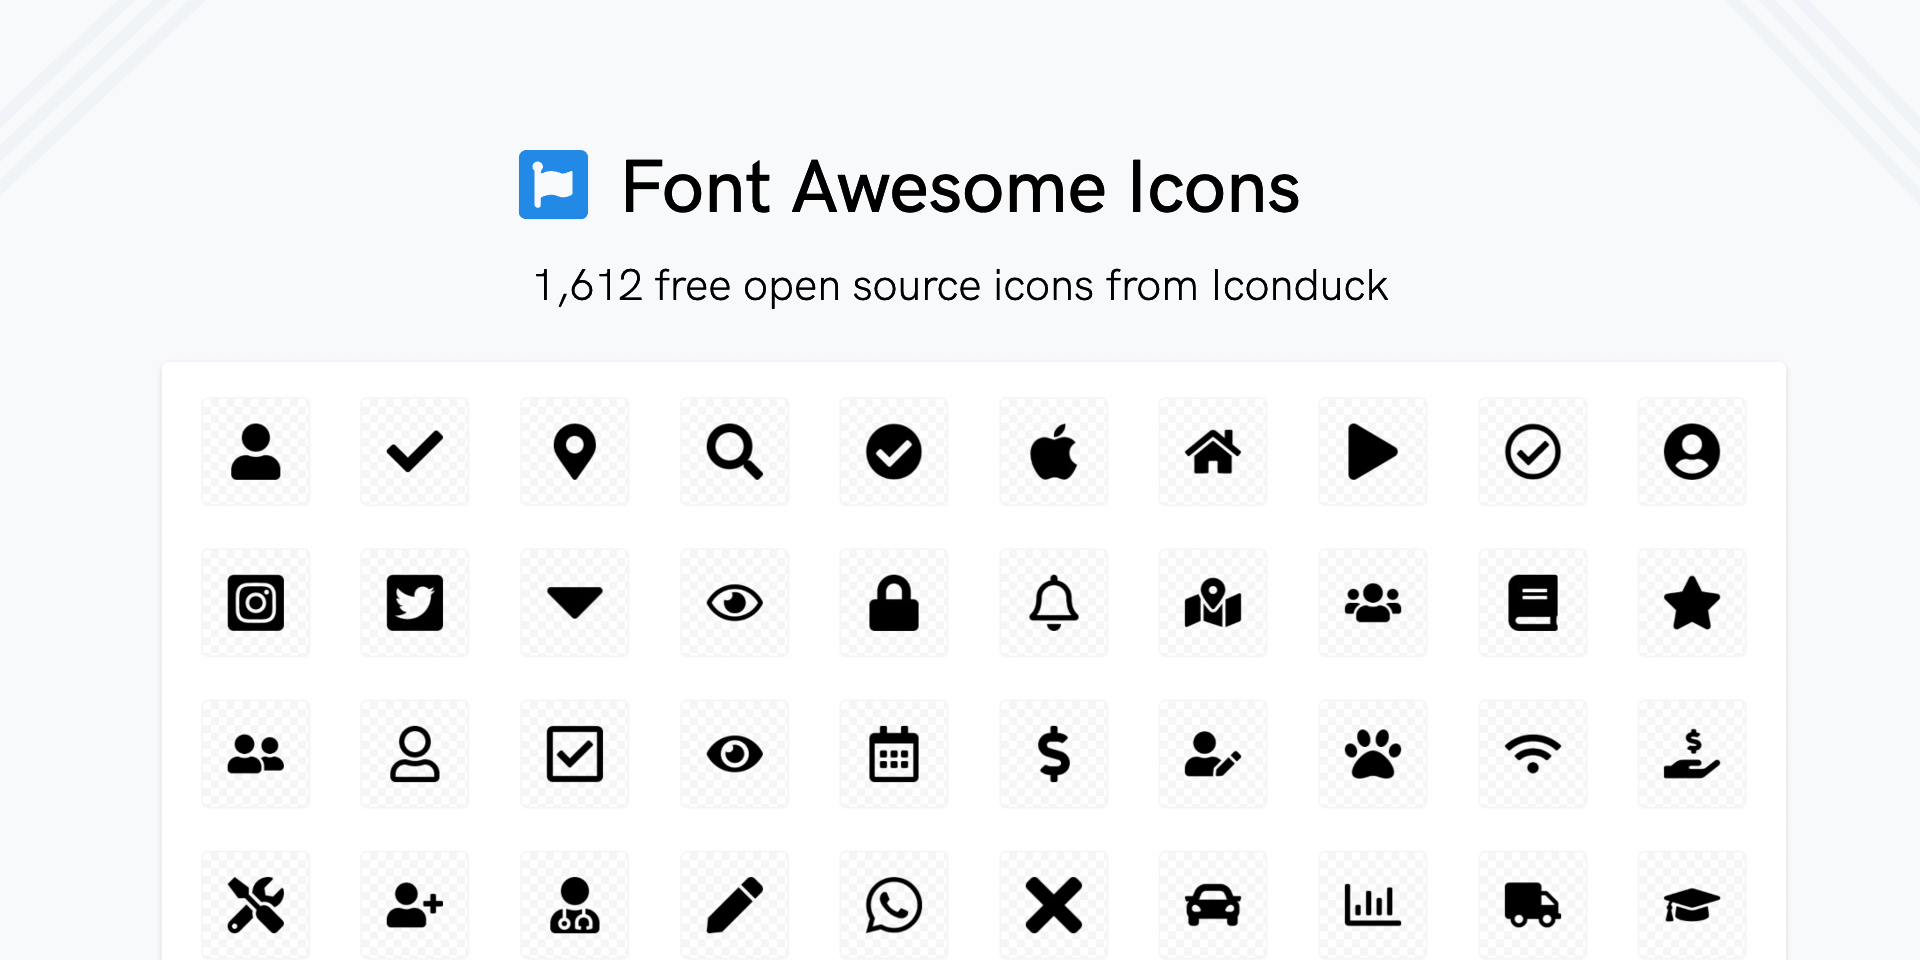
\includegraphics[width=15cm]{Figures/icons.PNG}
  \caption{La bibliothèque d'icons Font Awsome}
  %\label{fig:my_label} %Optional (If you want to reference the figure in later chapters)
\end{figure}











\subsection{La Conception d'Interfaces :}

\hspace{\parindent}Dans notre projet, Figma a joué un rôle central dans la conception des interfaces graphiques de Fawri-CMS. En tant qu'outil principal, il a offert une plateforme collaborative en temps réel ainsi que des fonctionnalités avancées pour créer des prototypes interactifs.

\textbf{Conception d'interfaces utilisateur} : Figma nous a permis de créer des maquettes et des prototypes interactifs pour les différentes interfaces de notre application, y compris les pages d'accueil, les formulaires de saisie de données, etc.

\textbf{Prototypage} : Grâce à ses fonctionnalités de prototypage avancées, nous avons pu simuler les interactions utilisateur et tester les flux de navigation avant le développement. Cela nous a permis d'identifier les problèmes d'expérience utilisateur et d'itérer rapidement sur les designs.
\\
\begin{figure}[H]
  \centering
  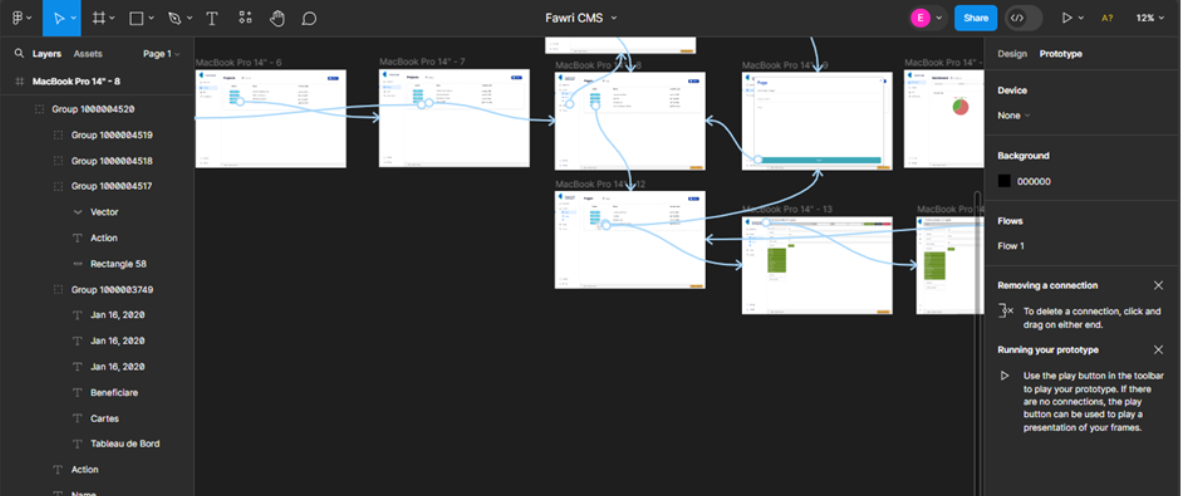
\includegraphics[width=17cm]{Figures/figma.PNG}
  \caption{La maquette d'interactivité de l'interface utilisateur de Fawri CMS}
  %\label{fig:my_label} %Optional (If you want to reference the figure in later chapters)
\end{figure}
















% \begin{longtable}[c]{| m{4.4cm} | m{11cm} |}
% \caption{Long table 1}\\
%  \hline

%  Cell & Description  \\ 
%  \hline
%  \endfirsthead

%  \hline

%  Cell & Description  \\ 
%  \hline
%  \endhead

%         \hline
%           Element11 & Element21 \\
%         \hline
%           Element12 & Element22 \\
%         \hline
%           Element13 & Element23 \\
%         \hline
%           Element14 & Element24 \\
%         \hline
%           Element15 & Element25 \\
%         \hline
%           Element16 & Element26 \\
%         \hline
%           Element17 & Element27 \\
%         \hline
%           Element18 & Element28 \\
%         \hline
%           Element19 & Element29 \\
%         \hline
%           Element110 & Element210 \\
%         \hline
%           Element111 & Element211 \\
%         \hline
%           Element112 & Element212 \\
%         \hline
%           Element113 & Element213 \\
%         \hline
%           Element114 & Element214 \\
%         \hline

%  \end{longtable}




\newpage

\section*{Conclusion}


\hspace{\parindent}Le chapitre d'Analyse et Conception a été une étape cruciale dans la planification de notre projet. En analysant les besoins, nous avons identifié les acteurs clés et détaillé les fonctionnalités du système, couvrant la gestion des utilisateurs, des tenants, des projets, du contenu et des autorisations. Dans la phase de Conception, nous avons élaborer des diagrammes pour illustrer l'architecture globale du système, ainsi qu'une charte graphique définissant l'identité visuelle du projet. Ces éléments fournissent une base solide pour le développement ultérieur, en assurant une compréhension claire des besoins des utilisateurs, une conception architecturale cohérente et une direction visuelle pour l'interface utilisateur.




























\chapter{Outils, Méthodologies et Architecture}
\label{chap:Chapter 3 title}
\section*{Introduction}

\hspace{\parindent}Le chapitre "Outils, Méthodologies et Architecture" revêt une importance capitale dans la contextualisation de notre projet. Il offre une vue d'ensemble précieuse sur les environnements technologiques dans lequel notre projet évolue, ainsi que sur les outils et les ressources nécessaires à sa réalisation.

Dans ce chapitre, nous détaillons les différents composants qui constituent notre environnement de développement et de test. Nous mettons en lumière les langages de programmation utilisés, les frameworks et les bibliothèques mobilisés, ainsi que les exigences matérielles et logicielles spécifiques au projet. De plus, nous abordons les méthodologies de travail et les concepts fondamentaux qui guident notre approche.

Cette connaissance approfondie de notre environnement et des outils disponibles nous a permis de prendre des décisions éclairées tout au long du processus de développement. Elle a également été cruciale pour optimiser notre architecture, garantissant ainsi la mise en place d'une solution robuste et efficace.

\newpage


\section{Langages de programmation}

\hspace{\parindent}Dans cette section, nous abordons les langages de programmation essentiels à notre projet, mettant en lumière leur rôle central dans le processus de développement. Nous nous concentrons sur l'importance de choisir des langages compatibles et cohérents pour garantir l'efficacité et la fluidité de notre travail tout au long du cycle de développement.

\textbf{C\#} : est un langage de programmation orienté objet et orienté composant. Ses structures de langage intègrent directement ces concepts, ce qui en fait un choix naturel pour la création et l'utilisation de composants logiciels. Depuis ses débuts, C\# a continué à évoluer en ajoutant des fonctionnalités pour répondre à de nouveaux cas d'utilisation et aux pratiques émergentes en conception logicielle. Ce choix est motivé par la robustesse, la clarté et la polyvalence de C\#, ainsi que par son intégration étroite avec la plateforme .NET. En utilisant C\#, nous bénéficions d'un langage moderne et éprouvé qui offre une grande productivité aux développeurs, une facilité de maintenance du code et une compatibilité avec un large éventail de technologies et de frameworks.
\\
\begin{figure}[H]
    \centering
    
\includegraphics[width=4cm]{Figures/csharp.png}
    \caption{C\#}
    %\label{fig:my_label} %Optional (If you want to reference the figure in later chapters)
\end{figure}


\textbf{SQL}, ou Structured Query Language, est un langage de programmation crucial pour interagir avec les bases de données. Il constitue un outil fondamental pour les développeurs web, leur permettant de gérer et de manipuler efficacement les données stockées dans les sites internet.
\\
\begin{figure}[H]
    \centering
    
\includegraphics[width=6cm]{Figures/sql.png}
    \caption{SQL}
    %\label{fig:my_label} %Optional (If you want to reference the figure in later chapters)
\end{figure}



\textbf{JavaScript} est utilisé de manière significative pour le développement d'applications web interactives. Nous l'utilisons pour améliorer l'expérience utilisateur en ajoutant des fonctionnalités dynamiques telles que des animations, des validations de formulaire en temps réel et des mises à jour de contenu sans rechargement de la page. De plus, JavaScript est utilisé pour intégrer des frameworks et des bibliothèques frontend populaires tels que React.js ou Angular.js, qui offrent des fonctionnalités avancées pour la création d'interfaces utilisateur réactives et complexes. En outre, JavaScript est également employé côté serveur avec Node.js pour gérer des tâches backend telles que la manipulation de
\\
\begin{figure}[H]
    \centering
    
\includegraphics[width=5cm]{Figures/javascript.png}
    \caption{JavaScript}
    %\label{fig:my_label} %Optional (If you want to reference the figure in later chapters)
\end{figure}






\section{Framework et bibliothèques}

\hspace{\parindent}Nous examinons les frameworks et les bibliothèques qui ont simplifié le développement de notre projet, en présentant les outils et les ressources qui contribuent à accroître notre efficacité et notre productivité. Nous mettons en lumière les avantages et les fonctionnalités de ces frameworks, qui joueront un rôle crucial dans la réalisation efficace de notre projet.

\textbf{Angular} : est un framework JavaScript développé par Google, largement reconnu pour sa capacité à créer des applications web dynamiques et interactives. Grâce à son architecture modulaire, Angular simplifie la gestion et la maintenance des grandes applications en les divisant en modules fonctionnels distincts. Cette approche organisée permet de rendre le code plus évolutif et facilite la collaboration entre les membres de l'équipe de développement. De plus, Angular offre un système de gestion de l'état robuste, assurant une synchronisation efficace entre les composants de l'interface utilisateur et les données du backend. Cette synchronisation cohérente des données contribue à offrir une expérience utilisateur fluide et réactive, même pour des applications complexes. Enfin, grâce à son moteur de rendu rapide et à sa gestion efficace de la mémoire, Angular garantit des performances optimales, ce qui est essentiel pour fournir une expérience utilisateur de haute qualité.
\\
\begin{figure}[H]
    \centering
    
\includegraphics[width=6cm]{Figures/angular.png}
    \caption{Angular framework}
    %\label{fig:my_label} %Optional (If you want to reference the figure in later chapters)
\end{figure}



\textbf{Node.js} : est un environnement d'exécution JavaScript côté serveur, basé sur le moteur JavaScript V8 de Google Chrome. Contrairement à d'autres environnements d'exécution JavaScript, Node.js permet d'exécuter du code JavaScript côté serveur, ce qui ouvre de nouvelles possibilités pour le développement d'applications web. Grâce à sa nature asynchrone et non bloquante, Node.js est particulièrement efficace pour gérer de nombreuses connexions simultanées, ce qui en fait un choix idéal pour les applications en temps réel telles que les applications de chat ou les tableaux de bord de données en temps réel. De plus, Node.js dispose d'un vaste écosystème de packages et de modules, disponibles via le gestionnaire de packages npm, ce qui facilite le développement et l'intégration de nouvelles fonctionnalités dans les applications. En outre, Node.js est extensible et peut être utilisé pour créer des applications web, des API RESTful, des applications de streaming, des outils en ligne de commande et bien plus encore. En résumé, Node.js est un outil puissant et polyvalent pour le développement d'applications côté serveur, offrant une performance élevée, une évolutivité et une flexibilité.
\\
\begin{figure}[H]
    \centering
    
\includegraphics[width=6cm]{Figures/nodejs.png}
    \caption{Node JS logo}
    %\label{fig:my_label} %Optional (If you want to reference the figure in later chapters)
\end{figure}






\textbf{ABP Framework (version 6.0)} : Le choix de ABP Framework (version 6.0) pour notre projet repose sur une série de facteurs clés qui garantissent la pertinence et l'efficacité de notre approche de développement.

ABP Framework est un cadre de développement open source conçu pour faciliter la création rapide et efficace d'applications web et mobiles modernes. Il offre une architecture solide et modulaire, ainsi qu'une multitude de fonctionnalités prêtes à l'emploi, permettant ainsi aux développeurs de se concentrer sur la logique métier de leurs applications plutôt que sur les aspects techniques.

Ce framework prend en charge plusieurs langages de programmation, notamment C\# pour le backend et TypeScript pour le frontend, offrant ainsi une flexibilité et une compatibilité avec les technologies modernes. De plus, ABP Framework intègre des bibliothèques populaires telles que Entity Framework Core pour la gestion des bases de données et Angular pour le développement de l'interface utilisateur, ce qui garantit la robustesse et la pérennité de notre solution.

L'un des avantages majeurs d'ABP Framework est sa capacité à fournir des modules prédéfinis, tels que Identity Server, qui simplifient le développement d'aspects critiques tels que l'authentification et l'autorisation. Cette approche modulaire et extensible permet aux développeurs de personnaliser facilement leurs applications en fonction de leurs besoins spécifiques, tout en bénéficiant d'une base solide et sécurisée.

Le choix d'ABP Framework pour notre projet s'inscrit dans une stratégie visant à optimiser le processus de développement, à garantir la qualité et la sécurité de notre solution, et à assurer sa pérennité à long terme
\\
\begin{figure}[H]
    \centering
    
\includegraphics[width=8cm]{Figures/abp.png}
    \caption{ABP framework logo}
    %\label{fig:my_label} %Optional (If you want to reference the figure in later chapters)
\end{figure}






\textbf{.NET} : .NET, en tant que plateforme open source, offre aux développeurs la possibilité de créer des applications pour les environnements de bureau, web et mobile. Ces applications sont conçues pour une exécution native sur une gamme étendue de systèmes d'exploitation. Ce choix est motivé par la polyvalence et la fiabilité de .NET, ainsi que par sa robustesse et son évolutivité. En tant que framework mature et largement adopté, .NET garantit une compatibilité avec de nombreuses technologies et une communauté de développeurs dynamique, ce qui facilite le développement, la maintenance et l'évolutivité de nos applications. De plus, l'écosystème .NET offre une vaste gamme de bibliothèques, d'outils et de services, ce qui nous permet de bénéficier d'une infrastructure solide pour la réalisation de notre projet.
\\
\begin{figure}[H]
    \centering
    
\includegraphics[width=8cm]{Figures/dotnet.png}
    \caption{.NET logo}
    %\label{fig:my_label} %Optional (If you want to reference the figure in later chapters)
\end{figure}




\textbf{Entity Framework (EF)} : est un Framework de mappage objet-relationnel (ORM) qui facilite l'accès et la manipulation des données dans les applications .NET. Il est intégré en tant qu'ORM par défaut dans ABP, simplifiant ainsi le développement d'applications avec une gestion efficace des données
\\
\begin{figure}[H]
    \centering
    
\includegraphics[width=6cm]{Figures/efcore.png}
    \caption{Entity Framework Core logo}
    %\label{fig:my_label} %Optional (If you want to reference the figure in later chapters)
\end{figure}


\textbf{Form.io Form Builder Open Source} : est un outil pour créer des formulaires web et des enquêtes de saisie de données. Il propose une interface intuitive de type glisser-déposer, une large gamme de composants de champs et des fonctionnalités avancées telles que la validation de données, la logique conditionnelle et la gestion de workflow.

Le Form Builder Open Source offre plusieurs fonctionnalités clés, notamment :

\begin{itemize}
    \item \textbf{Interface glisser-déposer conviviale} : Cette fonctionnalité simplifie la création de formulaires complexes en permettant l'assemblage intuitif des éléments via une interface glisser-déposer.

    \item \textbf{Variété de composants} : Le Form Builder Open Source offre un large éventail de composants de base, avancés et dédiés à la mise en page, permettant une construction personnalisée des formulaires selon les besoins spécifiques du projet.

    \item \textbf{Gestion intégrée des données} : Le form builder facilite la saisie et la gestion des données, avec la possibilité de soumettre directement les informations dans l'outil. De plus, il offre des fonctionnalités de visualisation et d'exportation des données au format JSON ou CSV pour une utilisation ultérieure.

    \item \textbf{Génération automatique d'API} : Cette fonctionnalité automatisée crée rapidement le schéma JSON et configure l'API nécessaire pour les formulaires, simplifiant ainsi le processus de développement et de test.
\end{itemize}

Dans ce projet, nous allons nous baser sur cette solution open source et l'adapter à nos besoins en ajoutant de nouveaux composants liés à nos processus spécifiques. Cette adaptation permettra d'enrichir les fonctionnalités du Form.io Form Builder et de mieux répondre aux exigences de notre application.
\\
\begin{figure}[H]
    \centering
    
\includegraphics[width=6cm]{Figures/dormiologo.png}
    \caption{Form.io logo}
    %\label{fig:my_label} %Optional (If you want to reference the figure in later chapters)
\end{figure}




\section{Outils et logiciels}


\textbf{SQL Server} : Le choix de base de données inclut également SQL Server, un système de gestion de base de données relationnelle (RDBMS). SQL Server, comme d'autres logiciels RDBMS, repose sur le langage de programmation standard appelé SQL (Structured Query Language), permettant ainsi d'interagir avec des bases de données relationnelles.
\\
\begin{figure}[H]
    \centering
    
\includegraphics[width=4cm]{Figures/sqlserver.png}
    \caption{Microsoft SQL Server logo}
    %\label{fig:my_label} %Optional (If you want to reference the figure in later chapters)
\end{figure}



\textbf{SQL Server Management Studio (SSMS)} : est nécessaire pour administrer la base de données SQL Server. Il s'agit d'un environnement intégré spécialement conçu pour la gestion de l'infrastructure SQL Server. SSMS propose une interface utilisateur conviviale ainsi qu'un ensemble d'outils, dont des éditeurs de scripts, permettant d'interagir efficacement avec SQL Server.
\\
\begin{figure}[H]
    \centering
    
\includegraphics[width=6cm]{Figures/sqlmanagementstudio.png}
    \caption{Microsoft SQL Server management studio logo}
    %\label{fig:my_label} %Optional (If you want to reference the figure in later chapters)
\end{figure}


\textbf{Visual Studio} : est un IDE complet développé par Microsoft, utilisé pour développer des applications informatiques, des sites web, des services web, des applications mobiles et bien plus encore. Il prend en charge plusieurs langages de programmation, notamment C\#, VB.NET, C++, Python, et d'autres. Visual Studio offre des outils de développement, de débogage et de test intégrés, ce qui en fait un choix populaire parmi les développeurs pour la création d'applications de haute qualité.
\\
\begin{figure}[H]
    \centering
    \includegraphics[width=4cm]{Figures/Visual-Studio-logo.png}
    \caption{Microsoft Visual studio logo}
    %\label{fig:my_label} %Optional (If you want to reference the figure in later chapters)
\end{figure}




\textbf{Visual Studio Code} : est un éditeur de code source léger mais puissant développé par Microsoft. Il offre aux développeurs un riche ensemble de fonctionnalités pour éditer, déboguer et gérer du code dans divers langages de programmation et plateformes. Nous l'avons largement utilisé pour le développement de nouvelles fonctionnalités dans Fawri Form. Son interface intuitive, son intégration Git intégrée et sa vaste bibliothèque d'extensions en ont fait le choix idéal pour notre workflow de développement. Grâce à VS Code, nous avons pu écrire, déboguer et tester du code de manière efficace, collaborer avec les membres de l'équipe en utilisant le contrôle de version et personnaliser notre environnement de développement en fonction de nos besoins spécifiques.
\\
\begin{figure}[H]
    \centering
    \includegraphics[width=2cm]{Figures/vsclogo.png}
    \caption{Microsoft Visual studio code logo}
    %\label{fig:my_label} %Optional (If you want to reference the figure in later chapters)
\end{figure}




\textbf{Git} : est un système de gestion de version largement utilisé dans le développement logiciel pour suivre les modifications apportées au code source durant la phase de développement. Il permet aux programmeurs de travailler simultanément sur un projet en suivant les différentes versions des documents ainsi que les modifications effectuées par plusieurs personnes. Git fonctionne dans l'environnement local d'un développeur, permettant de travailler en mode hors ligne et de faire des commits dans le référentiel local. Il offre également de solides fonctionnalités de branchement et de fusion, permettant aux utilisateurs de créer des branches pour les nouvelles fonctionnalités ou les corrections, qui peuvent ensuite être facilement fusionnées dans le flux principal de code. Git est capable de suivre les changements de code et sa structure de branchement permet la gestion des versions, la gestion du temps et le travail distribué. De plus, il fonctionne en conjonction avec de nombreux hébergeurs tels qu'Azure DevOps, GitHub, GitLab et Bitbucket pour le dépôt de code, le partage de code et le suivi de projet.
\\
\begin{figure}[H]
    \centering
    \includegraphics[width=8cm]{Figures/gitlogo.jpg}
    \caption{Git logo}
    %\label{fig:my_label} %Optional (If you want to reference the figure in later chapters)
\end{figure}



\section{Environnement de Test}


\textbf{xUnit.net} : Pour la réalisation des tests unitaires, nous avons opté pour le Framework xUnit.net. Il s'agit d'un outil open source dédié aux tests unitaires dans le cadre du .NET Framework et bénéficiant d'un fort soutien de la communauté. Conçu par l'inventeur original de NUnit v2, xUnit.net constitue la technologie de pointe en matière de tests unitaires pour les langages tels que C\#, F\#, VB.NET et autres langages .NET.
\\
\begin{figure}[H]
    \centering
    \includegraphics[width=6cm]{Figures/xunitlogo.png}
    \caption{xUnit.net logo}
    %\label{fig:my_label} %Optional (If you want to reference the figure in later chapters)
\end{figure}


\textbf{Swagger} : est un ensemble d'outils open source permettant de concevoir, de construire, de documenter et de consommer des services web RESTful. Il offre une interface conviviale pour décrire la structure des API REST, ainsi que la possibilité de générer automatiquement une documentation interactive à partir de ces descriptions. Swagger simplifie le processus de développement et de maintenance des API en fournissant une manière standardisée de définir et de partager les spécifications des API.
\\
\begin{figure}[H]
    \centering
    \includegraphics[width=6cm]{Figures/swaggerlogo.png}
    \caption{Swagger logo}
    %\label{fig:my_label} %Optional (If you want to reference the figure in later chapters)
\end{figure}



\section{Outils de conception et modélisation}


Dans ce projet, nous avons utilisé plusieurs outils pour la conception et la modélisation des différents aspects du système. Parmi ces outils, nous avons principalement utilisé UML (Unified Modeling Language). UML est un langage de modélisation visuelle standardisé, utilisé pour représenter les différents composants et interactions d'un système logiciel. Il permet de créer des diagrammes de cas d'utilisation, de classes, de séquence et bien d'autres, facilitant ainsi la compréhension et la conception du système.
\\
\begin{figure}[H]
    \centering
    \includegraphics[width=6cm]{Figures/UML_logo.svg.png}
    \caption{UML logo}
    %\label{fig:my_label} %Optional (If you want to reference the figure in later chapters)
\end{figure}

En plus de UML, nous avons également employé Figma, une plateforme de conception collaborative, pour créer des maquettes et des prototypes interactifs de l'interface utilisateur. Figma nous a permis de visualiser et de tester l'aspect visuel et l'ergonomie de l'application avant son développement.
\\
\begin{figure}[H]
    \centering
    \includegraphics[width=3cm]{Figures/figma logo.png}
    \caption{Figma logo}
    %\label{fig:my_label} %Optional (If you want to reference the figure in later chapters)
\end{figure}

En combinant ces outils, nous avons pu élaborer des représentations visuelles précises et détaillées de notre système, facilitant ainsi la communication et la collaboration entre les membres de l'équipe de développement.




\section{Concepts et Méthodologie}

Cette section offre une analyse approfondie des principes de conception logicielle et des méthodologies de développement les plus répandues. Nous y mettons en avant les meilleures pratiques de développement ainsi que les concepts fondamentaux qui guident la création de notre système.

\subsection{Test Driven Development}


\begin{figure}[H]
    \centering
    \includegraphics[width=6cm]{Figures/TDD.png}
    \caption{Cycle TDD}
    %\label{fig:my_label} %Optional (If you want to reference the figure in later chapters)
\end{figure}



Le Test-Driven Development (TDD), ou développement piloté par les tests, se démarque des approches traditionnelles par son approche inversée. Contrairement à la rédaction du code en premier lieu, le TDD met l'accent sur la création de tests automatisés qui spécifient le comportement attendu de chaque fonctionnalité. Ce processus itératif et incrémental se divise en trois étapes clés :
\begin{enumerate}

    \item \textbf{Rédiger un test qui échoue} : Le développeur commence par définir un test automatisé qui reflète le comportement souhaité de la fonctionnalité à implémenter. Ce test échoue initialement, car le code n'existe pas encore.

    \item \textbf{Écrire le code pour passer le test} : L'objectif est de développer le code minimal requis pour que le test automatisé précédemment créé réussisse. Il ne s'agit pas de produire un code parfait à ce stade, mais plutôt de répondre aux exigences essentielles du test.

    \item \textbf{Refactoriser le code} : Une fois le test réussi, le code est refactorisé pour améliorer sa structure, sa lisibilité et sa maintenabilité. Cette étape garantit que le code reste propre et évolutif, sans affecter le bon fonctionnement des tests.
\end{enumerate}

L'approche TDD offre de nombreux avantages :
\begin{itemize}
    \item \textbf{Amélioration de la qualité du code} : Les tests automatisés contraignent le développeur à écrire un code robuste et exempt de bugs.

    \item \textbf{Réduction des défauts} : En détectant les erreurs dès les premières étapes du développement, le TDD minimise le nombre de bugs à corriger ultérieurement.

    \item \textbf{Compréhension accrue des exigences} : Le processus de création de tests oblige le développeur à analyser et à clarifier les exigences fonctionnelles, menant à une meilleure compréhension du projet.
\end{itemize}

Ce projet est mis en place en respectant cette approche. Autrement dit, pour chaque intention obtenue à propos d’une fonctionnalité, un test est rédigé. Celui-ci échoue au début, mais après l’implémentation initiale de la fonctionnalité, il passe. Puis reste d’effectuer des refactorisations afin d’achever la fonctionnalité.



\subsection{Domain-Driven Design (DDD)}

Dans cette section, nous aborderons le Domain-Driven Design (DDD), une méthodologie de développement logiciel axée sur une compréhension approfondie et une modélisation précise du domaine métier d'une application. Contrairement à une approche uniquement technique, le DDD vise à harmoniser le code et la structure logicielle avec les concepts et le langage spécifiques au domaine concerné. Cette intégration permet aux développeurs de mieux répondre aux besoins et exigences propres au domaine, favorisant ainsi la création d'un code plus souple, modulaire et facilement maintenable.




Les principes clés du Domain-Driven Design (DDD) comprennent :
\begin{itemize}
    \item \textbf{Prioriser le domaine métier} : Le DDD positionne le domaine métier comme pilier central de la conception logicielle. Il incite les développeurs à s'immerger dans le domaine d'activité concerné, en collaborant étroitement avec les experts métier et en adoptant un langage commun pour décrire les concepts et processus métier.

    \item \textbf{Modélisation du domaine} : Au cœur de la démarche DDD se trouve la création d'un modèle du domaine métier. Ce modèle, tel un miroir du domaine réel, représente ses entités, agrégats, valeurs-objets, services et règles métier. Il sert à capturer les concepts clés du domaine et les interactions qui les lient, offrant une vision claire et structurée du système.

    \item \textbf{Bounded Contexts (Contextes limités)} : Le domaine métier peut être fragmenté en plusieurs contextes délimités, chacun possédant sa propre sémantique et ses règles métier spécifiques. Ces contextes délimités agissent comme des modules autonomes, favorisant la gestion de la complexité en délimitant les interactions entre les différentes parties du système.

    \item \textbf{Ubiquitous Language (Langage omniprésent)} : Le DDD met l'accent sur l'utilisation d'un langage commun, appelé "langage omniprésent", qui est partagé entre les experts métier et les développeurs. Ce langage permet de réduire les ambiguïtés et d'assurer une compréhension commune des concepts et des termes utilisés dans le domaine.

    \item \textbf{Agrégats} : Les agrégats représentent des ensembles d'objets étroitement liés, considérés comme une unité cohérente dans le modèle du domaine. Ils délimitent les transactions et assurent la cohérence des données.

    \item \textbf{Entités et Objets Valeur} : Les entités sont des objets ayant une identité distincte et se définissent par leurs attributs et comportements. Elles représentent des concepts avec des identités uniques et des cycles de vie propres au sein du domaine. En revanche, les objets valeur sont des objets dépourvus d'identité distincte et se définissent uniquement par leurs attributs. Ils représentent des valeurs ou des caractéristiques immuables au sein du domaine. Ensemble, les entités et les objets valeur constituent les éléments fondamentaux du modèle de domaine, chacun jouant un rôle spécifique pour capturer les nuances du domaine métier.
\end{itemize}

En adoptant les principes du DDD, nous pouvons concevoir des solutions logicielles mieux adaptées aux environnements complexes et aux applications de grande envergure.

Il existe quatre couches fondamentales dans une solution basée sur le Domain Driven Design (DDD).

\begin{figure}[H]
    \centering
    \includegraphics[width=9cm]{Figures/dddl.png}
    \caption{Les couches DDD}
    %\label{fig:my_label} %Optional (If you want to reference the figure in later chapters)
\end{figure}


\begin{itemize}
    \item \textbf{Couche Domaine (Domain Layer) :}
          \begin{itemize}
              \item Contient la logique métier centrale et indépendante des cas d'utilisation spécifiques.
              \item Implémente les règles, les entités, les valeurs objets et les agrégats qui définissent le cœur du système.
          \end{itemize}




    \item \textbf{Couche Application (Application Layer) :}
          \begin{itemize}
              \item Gère les cas d'utilisation de l'application en se basant sur les concepts du domaine.
              \item Ordonne et coordonne les opérations de domaine pour satisfaire les requêtes de l'utilisateur.
              \item Peut être considérée comme la couche qui orchestre les interactions utilisateur sur l'interface utilisateur (UI).
          \end{itemize}







    \item \textbf{Couche Présentation (Presentation Layer):}
          \begin{itemize}
              \item Comprend les éléments de l'interface utilisateur (UI), tels que les pages et les composants.
              \item Responsable de l'affichage des informations et de la gestion des interactions utilisateur.
          \end{itemize}






    \item \textbf{Couche Infrastructure (Infrastructure Layer) :}
          \begin{itemize}
              \item Supporte les autres couches en fournissant les abstractions et les intégrations nécessaires avec les bibliothèques tierces et les systèmes externes.
              \item Gère les aspects techniques tels que la persistance des données, les services externes, les messages et les événements.
          \end{itemize}

\end{itemize}



\subsection{Développement basé sur le tronc (Trunk-Based Development)}

\hspace{\parindent} Pour notre projet de fin d’études, nous avons adopté le développement basé sur le tronc (Trunk-Based Development, TBD) comme méthodologie de gestion de code source. Le TBD nous a permis d'intégrer fréquemment des modifications dans une seule branche principale, appelée "tronc" ou "master", ce qui a facilité une intégration continue et rapide, réduit les risques de conflits de fusion et soutenu une livraison continue efficace.

\begin{figure}[H]
    \centering
    \includegraphics[width=15cm]{Figures/tbd.png}
    \caption{Gestion des branches selon TBD}
    %\label{fig:my_label} %Optional (If you want to reference the figure in later chapters)
\end{figure}

L'approche TBD a plusieurs avantages:
\begin{itemize}

    \item \textbf{Intégration Continue} : En intégrant notre code régulièrement dans le tronc, nous avons pu détecter et résoudre précocement les conflits et les problèmes d'intégration.

    \item \textbf{Livraison Continue} : Cette approche a parfaitement complété notre pratique de livraison continue, nous permettant de déployer des mises à jour fréquentes et fiables.

    \item \textbf{Réduction des Conflits} : En évitant les branches de longue durée, nous avons minimisé les conflits de fusion, simplifiant ainsi notre processus de développement.

    \item \textbf{Collaboration Accrue} : En travaillant tous sur la même branche, nous avons favorisé une meilleure collaboration et une communication plus fluide au sein de notre équipe.

\end{itemize}





\subsection{Multitenancy : Une Architecture Efficace et Évolutive pour les Applications SaaS}



\hspace{\parindent}La \textit{multitenancy} est une approche dans laquelle une seule instance d'une application logicielle sert plusieurs organisations distinctes, appelées tenants. Chaque tenant opère comme s'il disposait de sa propre instance dédiée, avec des données et des configurations spécifiques, mais tous partagent la même infrastructure sous-jacente. Ses principes de base sont :

\begin{itemize}
    \item Isolation des Données : Les données de chaque tenant sont isolées pour garantir la confidentialité et la sécurité.

    \item Personnalisation : Chaque tenant peut personnaliser certains aspects de l'application (comme l'interface utilisateur et les configurations).

    \item Gestion des Ressources : Les ressources informatiques sont partagées entre les tenants, ce qui permet une utilisation plus efficace des ressources.

\end{itemize}


La \textit{multitenancy} présente plusieurs avantages, notamment dans le contexte des applications cloud et des services logiciels (SaaS). Voici quelques-uns des principaux avantages :

\begin{itemize}
    \item Efficacité des Coûts : Réduit les coûts d'infrastructure en partageant les mêmes ressources matérielles et logicielles entre plusieurs tenants.

    \item Facilité de Maintenance : Simplifie les mises à jour et la maintenance puisque les modifications apportées à une seule instance de l'application sont appliquées à tous les tenants.

    \item Évolutivité : Permet une montée en charge plus aisée en répartissant les coûts de développement et de maintenance sur plusieurs utilisateurs.

    \item Gestion Simplifiée : Facilite la gestion globale de l'application grâce à une seule base de code et une seule infrastructure.


\end{itemize}


\begin{figure}[H]
    \centering
    \includegraphics[width=9cm]{Figures/multytenancy.png}
    \caption{Le principe de la multitenancy}
    %\label{fig:my_label} %Optional (If you want to reference the figure in later chapters)
\end{figure}

\section{Architecture de la solution}

\subsection{Architecture de la solution Fawri-CMS suivant le DDD}

\hspace{\parindent}La figure suivante illustre un flux de demande typique pour une application web développée selon le DDD:


\begin{figure}[H]
    \centering
    \includegraphics[width=17cm]{Figures/DDD flow.png}
    \caption{L'architecture de la solution suivant DDD }
    %\label{fig:my_label} %Optional (If you want to reference the figure in later chapters)
\end{figure}


\begin{enumerate}
    \item Le navigateur de l'utilisateur envoie une requête HTTP au serveur web ;

    \item Le serveur web reçoit la requête et la transmet à l'application ;

    \item Dans la couche de présentation, le contrôleur ou le gestionnaire de requêtes traite la demande et Interagit avec les autres couches de l'application ;

    \item Le contrôleur ou le gestionnaire de requêtes interroge la couche d'application pour obtenir les données nécessaires pour répondre à la demande ;
    \item. Dans la couche d'application, les services applicatifs coordonnent l'exécution des cas d'utilisation métier ;

    \item Les services applicatifs utilisent la couche de domaine pour accéder aux entités, aux agrégats et aux règles métier ;

    \item La couche de domaine encapsule la logique métier et interagit avec la couche d'infrastructure pour récupérer ou persister les données ;

    \item La couche d'infrastructure communique avec le système de persistance (base de données, API externe, etc.) pour récupérer ou enregistrer les données ;

    \item Une fois que les données ont été récupérées, la couche d'infrastructure les renvoie à la couche d'application ;

    \item La couche d'application agrège les données et les prépare pour être renvoyées à la couche de présentation ;

    \item La couche de présentation utilise les données reçues pour générer une réponse appropriée à la requête initiale ;
    \item La réponse est renvoyée au serveur web qui la transmet ensuite au navigateur de l'utilisateur ;

    \item Le navigateur de l'utilisateur affiche la réponse dans l'interface utilisateur.
\end{enumerate}


Ce flux de demande suit les principes du DDD, où la logique métier est encapsulé dans la couche de domaine et la couche d'application coordonne l'exécution des cas d'utilisation. Les différentes couches travaillent ensemble pour fournir une réponse aux demandes des utilisateurs de l'application web.

\subsection{Architecture technique suivant le Template d’ABP}

\hspace{\parindent}Nous avons démarré le projet en utilisant ABP CLI pour générer la structure initiale. Ensuite, nous avons intégré le code dans un référentiel de versionnement hébergé sur Azure DevOps, ce qui nous permet de collaborer efficacement, de suivre les modifications du code et d'automatiser les processus de développement tels que l'intégration continue et la livraison continue (CI/CD).


Le projet est structuré en deux répertoires principaux : « src » et « test ». L'architecture de la solution est illustrée dans la figure suivante.



\begin{figure}[H]
    \centering
    \includegraphics[width=9cm]{Figures/src test.PNG}
    \caption{Structure du projet Fawri-CMS}
    %\label{fig:my_label} %Optional (If you want to reference the figure in later chapters)
\end{figure}


Chaque couche de l'architecture suit le principe SOLID (Single Responsibility), ce qui signifie qu'elle possède une seule responsabilité et un seul objectif de fonctionnement. ABP Framework, basé sur une architecture en couches, favorise une séparation claire des responsabilités et une modularité.

\begin{itemize}
    \item \textbf{Couche de présentation (Presentation Layer)} :

          Responsable de l'interface utilisateur de l'application, cette couche peut se présenter sous différentes formes telles qu'une application web, mobile, une API REST ou une interface utilisateur de bureau. Elle communique avec la couche d'application pour afficher les données et gérer les interactions utilisateur.\\

          \begin{figure}[H]
              \centering
              \includegraphics[width=9cm]{Figures/presentation layer.PNG}
              \caption{Couche Presentation}
              %\label{fig:my_label} %Optional (If you want to reference the figure in later chapters)
          \end{figure}

    \item \textbf{Couche d'application (Application Layer)} :

          Cette couche gère la logique métier de l'application. Elle contient les services d'application qui encapsulent les cas d'utilisation et les règles métier spécifiques. Les services d'application agissent comme une interface entre les couches supérieures et inférieures, orchestrant l'exécution des opérations de l'application.



          \begin{figure}[H]
              \centering
              \includegraphics[width=9cm]{Figures/application layer.PNG}
              \caption{Couche Application}
              %\label{fig:my_label} %Optional (If you want to reference the figure in later chapters)
          \end{figure}





    \item \textbf{Couche d'infrastructure (Infrastructure Layer)} :
          Fournit des services et des implémentations techniques pour soutenir les fonctionnalités de l'application. Elle comprend des classes utilitaires, des gestionnaires de persistance, des implémentations de fournisseurs de services tiers, des services d'authentification, des services de messagerie.

          \begin{figure}[H]
              \centering
              \includegraphics[width=9cm]{Figures/infra layer.PNG}
              \caption{Couche Infrastructure}
              %\label{fig:my_label} %Optional (If you want to reference the figure in later chapters)
          \end{figure}






    \item \textbf{Couche de domaine (Domain Layer)} :

          Représente le cœur de l'application. Elle définit les entités métier, les agrégats, les valeurs d'objet et les règles métier. Cette couche est indépendante de l'infrastructure et peut être réutilisée dans différents contextes d'application.

          \begin{figure}[H]
              \centering
              \includegraphics[width=9cm]{Figures/domain layer.PNG}
              \caption{Couche Domain}
              %\label{fig:my_label} %Optional (If you want to reference the figure in later chapters)
          \end{figure}

\end{itemize}



En plus des couches de DDD représentées par les projets situés dans le dossier src, nous avons également le dossier test (généré par ABP). Ce dossier contient les projets de tests, où nous écrivons et exécutons les tests pour notre projet. La capture d'écran fournie montre la structure du dossier test, avec plusieurs sous-projets :
\begin{figure}[H]
    \centering
    \includegraphics[width=9cm]{Figures/test folder.PNG}
    \caption{La structure du dossier \textit{test}}
    %\label{fig:my_label} %Optional (If you want to reference the figure in later chapters)
\end{figure}








\newpage
\section*{Conclusion}

\hspace{\parindent}Après avoir pris le temps d'explorer en profondeur l'architecture technique adoptée pour notre système à venir, ainsi que les différents outils et frameworks qui seront indispensables à sa réalisation, le prochain chapitre se penchera sur les étapes suivies pour donner vie à ce projet ambitieux.

\pagebreak


\selectlanguage{francais}


\chapter{Implémentation et Réalisation}
\label{chap:Chapter 4 title}
\section*{Introduction}

Dans ce chapitre, nous nous présentons les étapes du développement de l'application, en examinant de près les fonctionnalités intégrées ainsi que les ajustements opérés à chaque niveau du système.



\pagebreak

\section{Mise en place de l'environnement de développement}

\hspace{\parindent}Pour commencer le développement de l'application, nous avons initié la configuration de notre environnement de développement en installant une gamme d'outils et de frameworks essentiels tels que Visual Studio, .NET, ABP CLI, entre autres. En parallèle, nous avons également configuré la base de données et établi les connexions nécessaires pour assurer le bon fonctionnement de l'application. La Figure suivante présente l'installation de l'ABP CLI.

\begin{figure}[H] 
    \centering
    \includegraphics[width=17cm]{Figures/abp cli.PNG}
        \caption{ABP CLI}
    %\label{fig:my_label} %Optional (If you want to reference the figure in later chapters)
\end{figure}

\section{Couche de domaine (Domain Layer)}

Nous avons créé les entités décrites précédemment dans le projet \textbf{B3G.Fawri.CMS.Domain}.


\begin{figure}[H] 
    \centering
    \includegraphics[width=9cm]{Figures/domain folder.PNG}
        \caption{Structure du dossier Domain}
    %\label{fig:my_label} %Optional (If you want to reference the figure in later chapters)
\end{figure}

\section{Couche d'infrastructure (Infrastructure Layer)}

Dans cette couche, nous avons commencé par l'implémentation du contexte de base de données (DbContext) pour Entity Framework. Cette étape se divise en deux parties : la définition des DbSet et la configuration du modèle (builder).

Voici les configurations des builders pour les entités précédemment créées, réalisées dans le projet \textbf{B3G.Fawri.CMS.EntityFrameworkCore}.


\begin{figure}[H] 
    \centering
    \includegraphics[width=9cm]{Figures/entity fram core folder.PNG}
        \caption{Structure du dossier Infrastructure}
    %\label{fig:my_label} %Optional (If you want to reference the figure in later chapters)
\end{figure}


\begin{figure}[H] 
    \centering
    \includegraphics[width=17cm]{Figures/db set code.PNG}
        \caption{Configuration des DbSet}
    %\label{fig:my_label} %Optional (If you want to reference the figure in later chapters)
\end{figure}

\section{Couche d'application (Application Layer)}

Dans cette couche, nous créons les DTOs (Data Transfer Objects) et les interfaces de nos services dans le projet \textbf{B3G.Fawri.CMS.Application.Contracts} . Les DTOs servent de modèles pour transférer les données entre les couches de l'application, facilitant ainsi la communication sans exposer les entités du domaine directement.
\begin{figure}[H] 
    \centering
    \includegraphics[width=9cm]{Figures/dtos.PNG}
        \caption{Les DTOs dans la couche Application}
    %\label{fig:my_label} %Optional (If you want to reference the figure in later chapters)
\end{figure}

Ensuite, nous procédons à l'implémentation des services dans le projet \textbf{B3G.Fawri.CMS.Application}. Cette étape consiste à définir la logique métier spécifique aux cas d'utilisation de l'application, en respectant les contrats définis par les interfaces précédemment créées. L'implémentation des services inclut la gestion des opérations CRUD (Create, Read, Update, Delete), ainsi que toute autre logique métier nécessaire pour répondre aux exigences fonctionnelles de l'application.

\begin{figure}[H] 
    \centering
    \includegraphics[width=9cm]{Figures/services impl.PNG}
        \caption{Implementation des services}
    %\label{fig:my_label} %Optional (If you want to reference the figure in later chapters)
\end{figure}


Les Webservices implémentés sont : 


\begin{table}[H]
    \centering
    \begin{tabular}{|m{5cm}|m{10cm}|}
        \hline
          \textbf{Service} & \textbf{Description} \\
        \hline
          CreateProject & Ce WS permet de créer un projet \\
        \hline
          DeleteProject & Ce WS permet de supprimer un projet \\
        \hline
          ListProjects & Ce WS permet de récupérer la liste des projets \\
        \hline
        GetProjectById & Ce WS permet de récupérer un projet par son Id.\\
        \hline 
        UpdateProject & Ce WS permet de mettre à jour un projet.\\
        \hline
    \end{tabular}
    \caption{Les Web services de \textit{Project}}
\end{table}



\begin{table}[H]
    \centering
    \begin{tabular}{|m{5cm}|m{10cm}|}
      \hline
          \textbf{Service} & \textbf{Description} \\
    \hline
      CreatePage   & Ce WS permet de créer une page\\
      \hline
      DeletePage & Ce WS permet de supprimer une page.\\
      \hline
      ListPages & Ce WS permet de récupérer la liste des pages.\\
      \hline
GetPageById & Ce WS permet de récupérer une page par son Id.\\
\hline
UpdatePage & Ce WS permet de mettre à jour une page.\\
\hline
UpdatePageJson & Ce WS permet de mettre à jour une page en utilisant du JSON.\\
\hline
GetPagebySlug & Ce WS permet de récupérer une page par son slug.\\
\hline
GetSlugByPageId & Ce WS permet de récupérer le slug d'une page par son Id.\\
\hline
      
    \end{tabular}
    \caption{Les Web services de \textit{Page}}
    \label{tab:my_label}
\end{table}





\begin{table}[H]
    \centering
    \begin{tabular}{|m{5cm}|m{10cm}|}
    \hline
    \textbf{Service} & \textbf{Description} \\
    \hline
     CreateMenuItem & Ce WS permet de créer un élément de menu.\\
    \hline
    DeleteMenuItem & Ce WS permet de supprimer un élément de menu.\\
    \hline
    ListMenuItems & Ce WS permet de récupérer la liste des éléments de menu.\\
    \hline
    GetMenuItemById & Ce WS permet de récupérer un élément de menu par son Id.\\
    \hline
    UpdateMenuItem & Ce WS permet de mettre à jour un élément de menu.\\
    \hline
    \end{tabular}
    \caption{Les Web services de MenuItem}
    \label{tab:my_label}
\end{table}







\begin{table}[H]
    \centering
    \begin{tabular}{|m{5cm}|m{10cm}|}
    \hline
    \textbf{Service} & \textbf{Description} \\
    \hline
    CreateContentType & Ce WS permet de créer un type de contenu.\\
\hline
DeleteContentType & Ce WS permet de supprimer un type de contenu.\\
\hline
ListContentTypes & Ce WS permet de récupérer la liste des types de contenu.\\
\hline
GetContentTypeById & Ce WS permet de récupérer un type de contenu par son Id.\\
\hline

UpdateContentType & Ce WS permet de mettre à jour un type de contenu\\
\hline
    \end{tabular}
    \caption{Les Web services de ContentType}
    \label{tab:my_label}
\end{table}






\begin{table}[H]
    \centering
    \begin{tabular}{|m{5cm}|m{10cm}|}
    \hline
    \textbf{Service} & \textbf{Description} \\
    \hline
    CreateContentCategory & Ce WS permet de créer une catégorie de contenu. \\
    \hline
    DeleteContentCategory & Ce WS permet de supprimer une catégorie de contenu.\\
    \hline
    ListContentCategories & Ce WS permet de récupérer la liste des catégories de contenu\\
    \hline
    GetContentCategoryById & Ce WS permet de récupérer une catégorie de contenu par son Id.\\
    \hline
    UpdateContentCategory & Ce WS permet de mettre à jour une catégorie de contenu.\\
    \hline
    \end{tabular}
    \caption{Les Web services de ContentCategory}
    \label{tab:my_label}
\end{table}




\begin{table}[H]
    \centering
    \begin{tabular}{|m{5cm}|m{10cm}|}
    \hline
    \textbf{Service} & \textbf{Description} \\
    \hline
    CreateWidget & Ce WS permet de créer un widget \\
    \hline
    DeleteWidget & Ce WS permet de supprimer un widget.\\
    \hline

ListWidgets & Ce WS permet de récupérer la liste des widgets.\\
\hline

GetWidgetById & Ce WS permet de récupérer un widget par son Id.\\
\hline

UpdateWidget & Ce WS permet de mettre à jour un widget.\\

    \hline
    \end{tabular}
    \caption{Les Web services de Widget}
    \label{tab:my_label}
\end{table}














\begin{table}[H]
    \centering
    \begin{tabular}{|m{5cm}|m{10cm}|}
    \hline
    \textbf{Service} & \textbf{Description} \\
    \hline
    CreateProcess & Ce WS permet de créer un processus. \\
    \hline
    DeleteProcess & Ce WS permet de supprimer un processus.\\
    \hline

ListProcesses & Ce WS permet de récupérer la liste des processus.\\
\hline

GetProcessById & Ce WS permet de récupérer un processus par son Id.\\
\hline

UpdateProcess & Ce WS permet de mettre à jour un processus.\\

    \hline
    \end{tabular}
    \caption{Les Web services de Process}
    \label{tab:my_label}
\end{table}






\begin{table}[H]
    \centering
    \begin{tabular}{|m{5cm}|m{10cm}|}
    \hline
    \textbf{Service} & \textbf{Description} \\
    \hline
CreateItemView & Ce WS permet de créer une vue d'élément.\\
\hline

DeleteItemView & Ce WS permet de supprimer une vue d'élément.\\
\hline

ListItemViews & Ce WS permet de récupérer la liste des vues d'éléments.\\
\hline

GetItemViewById & Ce WS permet de récupérer une vue d'élément par son Id.\\
\hline

UpdateItemView & Ce WS permet de mettre à jour une vue d'élément.\\

    \hline
    \end{tabular}
    \caption{Les Web services de ItemView}
    \label{tab:my_label}
\end{table}



Après avoir implémenté les web services, nous démarrons le projet \textbf{B3G.Fawri.CMS.HttpApi.Host}. Cela lance Swagger, qui répertorie et documente tous les web services du système.

La figure suivante représente l’interface Swagger de notre solution :


\begin{figure}[H] 
    \centering
    \includegraphics[width=18cm]{Figures/swagger apis.PNG}
        \caption{Interface Swagger}
    %\label{fig:my_label} %Optional (If you want to reference the figure in later chapters)
\end{figure}


\section{Couche de présentation (Presentation Layer)}

\hspace{\parindent}Dans notre projet, la couche de présentation (Presentation Layer) joue un rôle crucial dans l'interaction entre l'utilisateur et l'application. Elle est responsable de l'affichage des informations et de la gestion des interactions utilisateur. Pour Fawri-CMS, le module \textbf{B3G.Fawri.CMS.Web} englobe toutes les interfaces utilisateur et les composants associés. C'est ici que nous créons nos pages (Razor Pages) et que nous gérons l'ensemble des éléments visuels et interactifs de l'application.



\begin{figure}[H] 
    \centering
    \includegraphics[width=9cm]{Figures/web folder.PNG}
    \caption{Structure du couche Web}
\end{figure}


Cette couche inclut divers dossiers et fichiers essentiels :

\begin{itemize}
    
 \item \textbf{Components} : Contient les composants réutilisables utilisés dans différentes parties de l'application.

 \item \textbf{Controllers} : Gère les requêtes HTTP et les interactions entre la vue et les modèles.

 \item \textbf{Menus} : Définit la structure de navigation de l'application.

 \item \textbf{Pages} : Contient les Razor Pages, qui sont les vues spécifiques de l'application.

 \item \textbf{TagHelpers} : Fournit des balises personnalisées pour simplifier la création de vues.

 \item \textbf{Themes} : Gère les thèmes et les styles visuels de l'application.

 \item \textbf{Views} : Contient les vues MVC traditionnelles, si nécessaire.

\end{itemize}




\section{Intégration d'Identity Server dans Fawri-CMS avec l'ABP Framework}

\hspace{\parindent}L'intégration d'Identity Server dans Fawri-CMS grâce à l'ABP Framework constitue un élément essentiel pour garantir la sécurité et la gestion efficace de l'identité des utilisateurs. Cette section explore en détail le fonctionnement de cette intégration et ses avantages pour notre application.

L'ABP Framework facilite l'intégration d'Identity Server en fournissant des fonctionnalités prêtes à l'emploi et des outils pour la gestion de l'authentification et de l'autorisation. Voici un aperçu du fonctionnement de cette intégration :

\begin{itemize}
    \item \textbf{Configuration de Identity Server} : L'ABP Framework simplifie la configuration d'Identity Server en fournissant des modèles et des outils pour définir les ressources, les clients et les utilisateurs autorisés à accéder à l'application.

\item \textbf{Gestion des utilisateurs et des rôles} : Grâce à ASP.NET Core Identity, qui est intégré à l'ABP Framework, la gestion des utilisateurs et des rôles est simplifiée. Identity Server utilise cette infrastructure pour authentifier les utilisateurs et leur attribuer les autorisations appropriées.

\item \textbf{Authentification basée sur les standards ouverts} : Identity Server prend en charge les protocoles d'authentification standard tels que OAuth 2.0 et OpenID Connect, assurant ainsi une authentification sécurisée et compatible avec les normes industrielles.

\item \textbf{Centralisation de l'authentification et de l'autorisation} : En intégrant Identity Server, Fawri-CMS bénéficie d'une solution centralisée pour gérer l'authentification et l'autorisation des utilisateurs, ce qui simplifie le développement et la maintenance de l'application.
\end{itemize}

Dans notre cas, nous avons choisi de séparer le serveur d'authentification en un projet distinct (\textbf{B3G.Fawri.CMS.AuthServer}) afin de pouvoir le personnaliser au fur et à mesure de l'avancement de ce projet.


\begin{figure}[H] 
    \centering
    \includegraphics[width=9cm]{Figures/login ui.PNG}
    \caption{Interface de l'authentification}
\end{figure}


\section{Gestion des tenants}

\hspace{\parindent}Dans notre solution Fawri-CMS, la gestion des tenants (ou multi-tenance) est un aspect crucial qui permet de servir efficacement plusieurs clients avec une seule instance de l'application. Grâce à l'ABP Framework, nous avons mis en place une architecture multi-tenant robuste qui offre isolation, personnalisation et sécurité pour chaque tenant.

Dans notre projet Fawri-CMS, nous avons implémenté la gestion des tenants en utilisant l'interface IMultiTenant fournie par l'ABP Framework. Chaque entité de notre application inclut un identifiant de tenant (TenantId), garantissant ainsi une isolation et une personnalisation des données pour chaque client (tenant).


\begin{figure}[H] 
    \centering
    \includegraphics[width=13cm]{Figures/tenant code.PNG}
    \caption{Implementation de la \textit{multitenancy}}
\end{figure}

% \section{Gestion des permissions}

% \hspace{\parindent}La gestion des permissions représente un pilier fondamental garantissant la sécurité et le contrôle d'accès à diverses fonctionnalités et ressources de notre application. Cette fonctionnalité permet de définir les droits d'accès des utilisateurs en fonction de leur rôle et de leurs responsabilités au sein de l'organisation, assurant ainsi une répartition adéquate des privilèges. Grâce à cette approche, les administrateurs disposent d'un contrôle précis sur les actions pouvant être effectuées par chaque utilisateur dans l'application.

% Par ailleurs, ABP Framework enrichit notre projet en mettant à disposition un module spécifique dédié à la gestion des permissions. Cette intégration harmonieuse offre une solution complète pour la définition et la gestion des autorisations. Le module permet une granularité fine dans la définition des permissions, permettant de spécifier des autorisations pour chaque action et ressource de l'application. De plus, il offre la souplesse nécessaire pour activer ou désactiver ces permissions en fonction des rôles, des utilisateurs ou des clients. Ainsi, notre équipe peut contrôler avec précision les actions autorisées pour chaque utilisateur, garantissant une gestion sécurisée et efficace des autorisations au sein de notre système.

\section{Interface d’utilisateur}

\subsection{Authentification de l’application :}

\hspace{\parindent}Lorsqu'un utilisateur, tel que le super administrateur (personnel de B3G) ou l'administrateur d'un tenant, souhaite accéder à la plateforme Fawri-CMS, le système lui demande de s'authentifier en fonction de son profil. La figure ci-dessous illustre la page de connexion.


\begin{figure}[H] 
    \centering
    \includegraphics[width=18cm]{Figures/full loging page.PNG}
    \caption{Page de l'authentification}
\end{figure}


\subsection{Interface Super Admin}

\hspace{\parindent}Le Super Admin est le pilier central de l'administration de Fawri-CMS. Il agit en tant que gardien principal de la plateforme, responsable de sa configuration initiale, de son bon fonctionnement quotidien et de son évolution continue. En tant que point focal, le Super Admin détient un ensemble de privilèges et de responsabilités étendus qui lui permettent de superviser tous les aspects de l'application.

Dans cette partie, nous allons présenter les fonctionnalités que seul le Super Admin peut effectuer, telles que la création d'éditions et de tenants. Le schéma suivant représente l'acheminement que nous allons suivre pour présenter les interfaces du Super Admin.

\begin{figure}[H] 
    \centering
    \includegraphics[width=11cm]{Figures/fonctionnalite super admin.PNG}
    \caption{Les fonctionnalités du super admin}
\end{figure}

\begin{enumerate}
    \item \textbf{Gestion des Éditions} :
    Dans Fawri-CMS, la gestion des éditions est une fonctionnalité essentielle qui permet au Super Admin de configurer et de personnaliser les offres pour différents segments de clients. Les éditions permettent de définir des niveaux de service distincts, chacun avec ses propres fonctionnalités et configurations spécifiques.

Le Super Admin a la responsabilité de créer, modifier et gérer les éditions. Ces éditions définissent les différentes versions de l'application qui peuvent être proposées à divers groupes de clients (tenants).

\begin{figure}[H] 
    \centering
    \includegraphics[width=17cm]{Figures/new edition.PNG}
    \caption{Interface d'ajout d'une édition}
\end{figure}

\item \textbf{Gestion des tenants} : 

\begin{figure}[H] 
    \centering
    \includegraphics[width=17cm]{Figures/tenant screenshot.PNG}
    \caption{Liste des tenants}
\end{figure}

\hspace{\parindent}Dans notre solution Fawri-CMS, le Super Admin a la possibilité de configurer la chaîne de connexion pour chaque nouveau tenant lors de sa création. Cette flexibilité permet de personnaliser la base de données utilisée par chaque tenant, garantissant une isolation appropriée des données et une gestion efficace des ressources. Le Super Admin peut également choisir d'utiliser la chaîne de connexion par défaut pour les nouveaux tenants si aucune personnalisation spécifique n'est nécessaire.



\item \textbf{Connexion en tant que tenant} :

Étant donné que le Super Admin a un contrôle total de l'application, il peut se connecter en tant que tenant. De plus, il a accès à toutes les fonctionnalités de l'application.




\end{enumerate}


\subsection{Interface Tenant}

Dans cette partie, nous allons présenter les fonctionnalités spécifiques au Tenant Admin. Ces fonctionnalités incluent la gestion des projets, la gestion de contenu, la gestion des utilisateurs et des permissions au sein de leur propre espace de travail (tenant). Le Tenant Admin joue un rôle crucial en administrant et en personnalisant les paramètres et les ressources disponibles pour les utilisateurs finaux dans leur tenant.



% \begin{figure}[H] 
%     \centering
%     \includegraphics[width=17cm]{Figures/tenant screenshot.PNG}
%     \caption{Interface de l'authentification}
% \end{figure}

\begin{enumerate}
    \item \textbf{Création d’un nouveau projet} :
    


\begin{figure}[H] 
    \centering
    \includegraphics[width=10cm]{Figures/new project.PNG}
    \caption{Création d'un nouveau projet}
\end{figure}

\begin{figure}[H] 
    \centering
    \includegraphics[width=17cm]{Figures/list projects.PNG}
    \caption{Consultation des projets}
\end{figure}



\item \textbf{Gestion des pages} :

\begin{figure}[H] 
    \centering
    \includegraphics[width=17cm]{Figures/list pages.PNG}
    \caption{Consultation des pages}
\end{figure}


\begin{figure}[H] 
    \centering
    \includegraphics[width=17cm]{Figures/manage page.PNG}
    \caption{Gestion des pages}
\end{figure}


En plus des composants de base de cet éditeur basé sur Form.io, nous avons ajouté un nouveau composant "Process" dans la section Premium (voir figure suivante). Ce composant nous permet d'utiliser les processus créés avec Fawri-Flow, favorisant ainsi la réutilisation des composants et des processus existants au lieu de les développer à partir de zéro. Ce composant "Process" récupère la liste des processus créés avec Fawri-Flow et nous permet de les intégrer facilement à nos pages.



\begin{figure}[H] 
    \centering
    \includegraphics[width=9cm]{Figures/process 1.PNG}
    \caption{Organisation des Processus}
\end{figure}
\begin{figure}[H] 
    \centering
    \includegraphics[width=17cm]{Figures/process 2.PNG}
    \caption{Ajout du processus \textit{SignatureWithOtp}}
\end{figure}

Le processus sélectionné est ajouté à la page. Dans notre cas, nous avons choisi le processus du service vérification avec OTP comme exemple.

Après la création de notre page, on clique sur "Save" pour sauvegarder la page créée (sauvegarder le JSON généré) et on visualise la page en cliquant sur "Preview".


\item \textbf{La gestion des menus} : 
Après la création et l'édition des pages, nous passons à la création des éléments de menu. Cela se fait en attribuant les éléments de menu soit à une page créée dans notre projet, soit à une URL externe.

\begin{figure}[H] 
    \centering
    \includegraphics[width=12cm]{Figures/menu item.PNG}
    \caption{L'ajout d'un élément au menu}
\end{figure}

Lors de la création d'un élément de menu dans notre projet Fawri-CMS, nous avons la possibilité de l'affecter à une page spécifique que nous avons créée, ou de le lier à une URL externe. De plus, il est possible de créer des sous-menus pour structurer le contenu de manière hiérarchique. Cette flexibilité permet une personnalisation et une organisation optimale de la navigation au sein de l'application, améliorant ainsi l'expérience utilisateur.




\item \textbf{La gestion des permissions} : 


La gestion des permissions, qui consiste à définir les droits d'accès à différents niveaux, est essentielle dans tout système. Elle implique notamment la mise en place de rôles tels que le super administrateur, qui détient des privilèges étendus sur l'ensemble du système, et l'administrateur du locataire (Tenant Admin), chargé de gérer les autorisations au niveau spécifique du locataire.

\begin{figure}[H] 
    \centering
    \includegraphics[width=17cm]{Figures/permission.PNG}
    \caption{Gestion des permissions}
\end{figure}





\end{enumerate}



















\newpage

\section*{Conclusion}

\hspace{\parindent}Le chapitre portant sur l'Implémentation et la Réalisation a constitué une étape fondamentale de notre projet, marquant son passage de l’analyse et la conception à la mise en œuvre opérationnelle. Nous avons commencé par établir un environnement de développement adéquat, puis avons exploré en profondeur les différentes couches de l'architecture logicielle, assurant ainsi une base solide pour notre application. L'intégration d'Identity Server dans Fawri-CMS grâce à l'ABP Framework a permis de garantir la sécurité et la gestion efficace de l'authentification des utilisateurs. De plus, la mise en place de la gestion des tenants et des permissions a offert une flexibilité et une adaptabilité indispensables à notre système. À travers le développement d'une interface utilisateur intuitive pour les Super Admins et les Tenants, nous avons veillé à ce que l'expérience utilisateur soit optimale et conviviale. En somme, ce chapitre a été crucial pour matérialiser notre projet, en fournissant les bases techniques et fonctionnelles nécessaires à son succès et à sa pérennité.

\pagebreak

%\chapter{Chapter 5 title}
\label{chap:Chapter 5 title} 
\section*{Introduction}

Lorem ipsum dolor sit amet, consectetur adipiscing elit. Praesent nec dapibus justo. Donec sagittis vulputate ante sed porttitor. Suspendisse sit amet nisl massa. Curabitur nec nisl condimentum, egestas ex vitae, dapibus enim. Etiam iaculis, erat faucibus pellentesque sagittis, nisi justo sollicitudin nibh, et condimentum augue massa non turpis. Proin commodo enim fermentum suscipit condimentum. Maecenas molestie, dui nec vestibulum rhoncus, arcu nisl faucibus neque, a ornare nisi massa ac eros. Aenean id velit sit amet lacus mattis varius. Donec fringilla massa sed nisi eleifend, a aliquet mi tempus. Nunc posuere euismod est, nec tristique augue lobortis non. Sed sodales sem ut metus tempus ullamcorper.

\pagebreak

\section{Section1}

\subsection{Subsection1}

\subsection{Subsection2}

\subsubsection{Subsubsection1}

\subsubsection{Subsubsection2}

\paragraph{Paragraph a}

\paragraph{Paragraph b}

\section{Section2}

\subsection{Subsection1}

\subsection{Subsection2}

\subsubsection{Subsubsection1}

\subsubsection{Subsubsection2}

\paragraph{Paragraph a}

\paragraph{Paragraph b}









\newpage
\section*{Conclusion}

Lorem ipsum dolor sit amet, consectetur adipiscing elit. Praesent nec dapibus justo. Donec sagittis vulputate ante sed porttitor. Suspendisse sit amet nisl massa. Curabitur nec nisl condimentum, egestas ex vitae, dapibus enim. Etiam iaculis, erat faucibus pellentesque sagittis, nisi justo sollicitudin nibh, et condimentum augue massa non turpis. Proin commodo enim fermentum suscipit condimentum. Maecenas molestie, dui nec vestibulum rhoncus, arcu nisl faucibus neque, a ornare nisi massa ac eros. Aenean id velit sit amet lacus mattis varius. Donec fringilla massa sed nisi eleifend, a aliquet mi tempus. Nunc posuere euismod est, nec tristique augue lobortis non. Sed sodales sem ut metus tempus ullamcorper.


\chapter*{Conclusion générale}


% This conclusion is unnumbered, if you want it numbered, you can remove the * from above and remove the line below, so it becomes a chapter, then add sections.

\addcontentsline{toc}{chapter}{Conclusion générale } %adds to the table of contents 

\label{chap:General Conclusion} 

\hspace{\parindent}En conclusion, le projet de développement de Fawri-CMS a représenté une étape significative dans notre parcours académique et professionnel. À travers ce projet, nous avons non seulement atteint les objectifs fixés initialement, mais nous avons également surmonté des défis techniques et acquis des compétences précieuses tout au long du processus.

La réussite de Fawri-CMS repose sur plusieurs facteurs clés, notamment la simplification du processus de développement, l'intégration transparente des processus métier, la réduction du temps et des ressources nécessaires au développement, ainsi que la démocratisation de l'accès au développement d'applications. Ces succès ont été reconnus lors du prestigieux "Saudi No Code Innovation Summit", organisé du 20 au 21 mai 2024 en Arabie Saoudite, mettant en évidence la pertinence et l'innovation de notre projet dans le domaine du développement logiciel.

Nous avons également consolidé nos compétences techniques et professionnelles grâce à une formation intensive suivie d'une expérience pratique, ce qui nous a préparés de manière proactive à relever les défis du monde professionnel.

En envisageant les perspectives d'évolution pour Fawri-CMS, nous avons identifié des opportunités stratégiques pour renforcer sa robustesse, son efficacité et sa valeur pour les utilisateurs. Parmi les pistes à explorer figurent des améliorations techniques, une meilleure expérience utilisateur et la mise en place d'un système de facturation transparent. Nous prévoyons également d'intégrer des fonctionnalités avancées telles que la publication des applications créées par les clients, la création d'éditions différenciées en termes de fonctionnalités, et l'ajout de templates pour faciliter la personnalisation et l'adoption de la plateforme. De plus, nous envisageons de permettre aux utilisateurs de créer leurs propres processus et composants directement dans Fawri-CMS, renforçant ainsi leur autonomie et leur capacité à personnaliser la solution selon leurs besoins spécifiques. Ces initiatives garantiront le succès continu et l'impact positif de Fawri-CMS sur le marché.

En définitive, ce projet de fin d'études nous a permis de démontrer notre capacité à concevoir, développer et faire évoluer une solution logicielle innovante, tout en enrichissant notre bagage professionnel pour les défis à venir dans le domaine du développement logiciel. Nous sommes fiers des réalisations accomplies et confiants dans le potentiel de croissance et d'impact de Fawri-CMS sur le marché.


%\section{Optional Section}

\appendix



% \chapter{Some subject you want to expand on}
\label{chap:Some subject you want to expand on} 


You can add more appendices depending on the subjects.
%You can decide which code snippets to use in the main report and which to add here in the annex
    
    \lstset{style=mystyle} %this style is already defined in Packages.tex
    
    \begin{lstlisting}[language=bash, caption= Bash example]
    
    [root@host ~]# You can change the language and caption.

    \end{lstlisting}



    \begin{lstlisting}[language=python, caption= Python example]
    
    # Solve the quadratic equation ax**2 + bx + c = 0

    # import complex math module
    import cmath
    
    a = 1
    b = 5
    c = 6
    
    # calculate the discriminant
    d = (b**2) - (4*a*c)
    
    # find two solutions
    sol1 = (-b-cmath.sqrt(d))/(2*a)
    sol2 = (-b+cmath.sqrt(d))/(2*a)
    
    print('The solution are {0} and {1}'.format(sol1,sol2))

    \end{lstlisting}



\begin{table}[H]
    \centering
    \begin{tabular}{|m{5cm}|m{10cm}|}
        \hline
          Column1 & Column2 \\
        \hline
          Element11 & Element21 \\
        \hline
          Element12 & Element22 \\
        \hline
          Element13 & Element23 \\
        \hline
    \end{tabular}
    \caption{Table Example}
\end{table}




\begin{longtable}[c]{| m{4.4cm} | m{11cm} |}
\caption{Long table Example}\\
 \hline

 Cell & Description  \\ 
 \hline
 \endfirsthead

 \hline
 
 Cell & Description  \\ 
 \hline
 \endhead

        \hline
          Element11 & Element21 \\
        \hline
          Element12 & Element22 \\
        \hline
          Element13 & Element23 \\
        \hline
          Element14 & Element24 \\
        \hline
          Element15 & Element25 \\
        \hline
          Element16 & Element26 \\
        \hline
          Element17 & Element27 \\
        \hline
          Element18 & Element28 \\
        \hline
          Element19 & Element29 \\
        \hline
          Element110 & Element210 \\
        \hline
          Element111 & Element211 \\
        \hline
          Element112 & Element212 \\
        \hline
          Element113 & Element213 \\
        \hline
          Element114 & Element214 \\
        \hline

 \end{longtable}


\begin{thebibliography}{99}
    \addcontentsline{toc}{chapter}{Bibliographie}


    \bibitem{ref1}
    \emph{Site web B3G} :
    \href{https://b3gtech.com/}{\textbf{www.b3gtech.com}}

    \bibitem{ref2}
    \emph{Page des produits et solutions B3G} :
    \href{https://b3gtech.com/fawri-suite/}{\textbf{Fawri Suite}}

    %the link is a documentation of the basic bibliography method (that    I'm using here) + bibTex which is more advanced, read it well and decide which one works best for you.

    \bibitem{ref3}
    \emph{WordPress} :
    \href{https://wordpress.com/fr/}{\textbf{Site web WordPress}}

    \bibitem{ref4}
    \emph{Drupal} :
    \href{https://www.drupal.org/}{\textbf{Site web Drupal}}

    \bibitem{ref5}
    \emph{Joomla} :
    \href{https://www.joomla.fr/}{\textbf{Site web Joomla}}

    \bibitem{ref6}
    \emph{SiteCore} :
    \href{https://www.sitecore.com/}{\textbf{Site web SiteCore}}

    \bibitem{ref7}
    \emph{ABP} :
    \href{https://abp.io/}{\textbf{Site web ABP framework}}

    \bibitem{ref8}
    \emph{Form.io Form Builder} :
    \href{https://form.io/}{\textbf{Form.io}}

    \bibitem{ref9}
    \emph{DDD Layers \& Clean Architecture} :
    \href{https://docs.abp.io/en/abp/4.2/Domain-Driven-Design-Implementation-Guide}{\textbf{Implementation DDD avec ABP framework}}



\end{thebibliography}

\end{document}